\documentclass{article}
\usepackage[utf8]{inputenc}
\usepackage[french]{babel}
\usepackage{frbib}
\usepackage{french}

\usepackage{xfrac}
\usepackage{algorithm}
\usepackage[noend]{algpseudocode}
\usepackage{geometry}
\usepackage{amssymb}
\usepackage{pgfplots}
\pgfplotsset{width=10cm,compat=1.9}


\geometry{
	a4paper,
	left=30mm,
	top=30mm,
}
\usepackage{hyperref}
\graphicspath{ {./img/} }
\usepackage{pgf}
\usepackage{tikz}
\usetikzlibrary{arrows,automata}
\usepackage{tikz-qtree}

\newcommand{\subsubsubsection}[1]{\paragraph{#1}\mbox{}\\}
\setcounter{secnumdepth}{4}
\setcounter{tocdepth}{4}


\newenvironment{citationbox}
{\begin{center}
		\begin{minipage}{.8\textwidth}
		}
		{
		\end{minipage}	
\end{center}
}

\title{Littérature et algorithmes~: une remise en question de la littérarité~?}
\author{Adèle Mortier}

\begin{document}
	\nocite{*}
	\maketitle
	\tableofcontents
	\newpage
	\section*{Introduction générale}
	\begin{center}
		\begin{minipage}{.8\textwidth}
			\textit{Alice est portée en avant par ses souvenirs, ramenée par eux en arrière... Elle est menée du dedans par ses souvenirs, à mesure qu'ils lui reviennent à l'esprit et ils reviennent en désordre. Ils prennent leurs distances. Pourra-t-elle jamais acquérir la sérénité~?... Le vent fait balancer les voiles de mousseline. La ville entière ne cesse de parler d'un assassinat qui aurait été commis la veille. Vie et Mort sont intimement liées comme les deux têtes de sœurs siamoises dont les voix discordantes ne disent différemment que pensées d'un même cerveau. Tout est littérature, seule la fiction approche la vérité.}
			\begin{flushright}
				Jean-Pierre Balpe, \textit{Un roman inachevé}, p.558 \cite{balpe1994}
			\end{flushright}
		\end{minipage}
	\end{center}
	
		On a souvent dit que le langage, au même titre que l'art, était le propre de l'homme. L'homme serait le seul être vivant à pouvoir transmettre efficacement et immédiatement des informations complexes et abstraites le concernant ou touchant à son environnement, et ce à travers des canaux divers~: canal auditif (voix), canal visuel (écriture, langues signées), canal sensoriel (écriture braille). Or, la recherche en sciences cognitives et  en linguistique a montré au cours des dernières décennies la complexité du langage de certains animaux, les singes bien évidemment\cite{schlenker2014}, mais aussi certains oiseaux ou cétacés\cite{dehaene2017}, et même les insectes. Qu'en est-il dès lors de notre avantage cognitif, jusque là indubitable~?\\
		
		Nous pensons pouvoir trouver deux aspects de notre langage qui le distinguent encore de celui des `` bêtes ''. Le premier aspect, plus littéraire, touche à la sémantique, voire à l'herméneutique~: rappelons-nous pour cela des six fonctions canoniques du langage énoncées par Roman Jakobson au début de la second moitié du XX$^{eme}$ siècle \cite{jakobson1960}~: fonction expressive, conative, phatique, métalinguistique, référentielle, et enfin, fonction poétique. Parmi ces fonctions, la fonction poétique du langage est sans doute la plus profondément humaine car détachée des contraintes biologiques. Cette fonction, étymologiquement fonction de \textit{création}, s'attache aux caractéristiques formelles du message, qui s'incorporent voire se substituent à ce dernier. En ce sens, le langage humain comprend une composante esthétique et processuelle.\\
		
		Le second facteur de différentiation que nous pensons pouvoir dégager, plus technique, touche au potentiel de formalisation du langage et à la notion de complexité qui en découle. Pour mieux comprendre cette notion, il faut s'intéresser évidemment aux travaux de Noam Chomsky, père de la linguistique formelle moderne. Chomsky, en développant la théorie des grammaires génératives, élabora une hiérarchie des langages à quatre niveaux \cite{chomsky1956}, selon la permissivité des règles de productions syntagmatiques (et ce faisant leur pouvoir d'expression). L'homme, dans sa pratique du langage, serait capable de maîtriser tous les niveaux, alors que le singe par exemple, ne pourrait atteindre les niveaux super-réguliers\footnote{un exemple ``canonique'' de langage super-régulier et le langage des mots commençant par $n$ éléments identiques suivis de $n$ autres éléments identiques; dénoté en général $a^nb^n$. Ce type de langage requiert une connaissance d'un contexte ``élargi'', dans le sens où il impose de ``compter'' les caractères identiques placés les uns à la suite des autres. Les singes en général ne sont pas en mesure de reconnaître et d'imiter ce genre de motif complexe.}\footnote{certaines analyses du langage des singes en termes minimalistes \cite{chomsky1995} s'attachent à dire que le niveau des signes est en quelque sorte ``intermédiaire''; ils posséderaient une variété de \textit{merge} ``non récursif'' \cite{dehaene2017}...}. Or la maîtrise ou la non maîtrise de grammaires complexes influe directement sur la complexité des phrases (en particulier sur la possibilité d'introduire des dépendance référentielles dites à longue distance \cite{shieber1985}...).\\
		
		Le langage humain se démarque donc tant sur son intention que sur son pouvoir d'expression; c'est aussi une faculté ancrée au plus profond de nous, et qui pour une part tout au moins, semble inscrite dans nos gènes\cite{pinker2008}. 
		\begin{citationbox}
			\textit{En un mot, ``faire faire'' de la littérature à une machine, et plus encore de la poésie, est parfois ressenti comme sacrilège car assimilé à un abandon de notre part la plus humaine, celle qui exprime le vrai, le juste et, surtout, tous nos sentiments.}
			\begin{flushright}
				Philippe Bootz, \textit{Les Basiques~: la littérature numérique} \cite{bootz2006}
			\end{flushright}
		\end{citationbox}
		Et pourtant, la recherche en informatique (et plus précisément en apprentissage statistique) ne cesse aujourd'hui de progresser et de produire des textes de plus en plus réalistes, si bien que l'on se demande parfois à qui l'on parle. Par exemple, certains outils de conversation (\textit{chatbots}, assistants à commande vocale...) résistent toujours plus au test de Turing \cite{guilet2017}\footnote{Dans l'\textit{Instinct du langage} de Steven Pinker \cite{pinker2008}, l'auteur mentionne des ``concours de \textit{chat}'' entre humains et robot dès les années 90. Le but étant pour les robots de converser sept minutes de façon ``naturelle'' avec les juges sans se faire démasquer, autrement dit, il s'agissait de passer et de réussir le test de Turing.}\footnote{A voir également~: cette récente présentation de Google, où l'assistant vocal d'Android prend un rendez-vous chez le coiffeur et une table dans un restaurant, sans que les interlocuteurs se doutent qu'ils parlent à une IA... \href{https://www.youtube.com/watch?v=D5VN56jQMWM}{https://www.youtube.com/watch?v=D5VN56jQMWM}}. Et cette capacité croissante des ordinateurs à simuler le langage humain ne touche pas que le domaines ``triviaux'' du quotidien ; bien au contraire, elle s'applique de plus en plus fréquemment à un langage qui justement exploite à l'envi la fonction poétique~: le langage littéraire.\\
		
		Nous croiriez-vous par exemple, si l'on vous annonçait que le texte mis en exergue de ce document était un texte généré par ordinateur~? Comment expliquer cette impression de paradoxe, ce malaise qui résulte parfois de notre interaction avec les IAs (intelligences artificielles)~? Les avancées techniques et conceptuelles appartenant à la sphère de l'intelligence artificielle pourraient en effet nous conduire à remettre en question l'idée même de littérarité. Et il faudrait dès lors aboutir à de nouveaux critères, des critères propres à discriminer un texte issu d'un ordinateur d'une texte produit par une conscience humaine. Mais de là survient aussi une autre question, peut être plus dérangeante encore~: en est-on arrivé à un point ou ce n'est plus l'ordinateur qui imite l'homme, mais l'homme qui imite l'ordinateur~?\\
		
		Nous tenterons de répondre à ces questions dans cet exposé, qui suivra trois mouvements. Dans un premier temps, nous poserons le cadre de l'étude en retraçant l'histoire de l'écriture dite ``générative'' jusqu'à la génération de texte par ordinateur que l'on connaît de nos jours. Nous étudierons dans une seconde partie l'état de l'art en la matière, selon un point de vue plus technique. Enfin, nous aborderons les aspects plus philosophiques et ontologiques du problème, et notamment la relation entre l'homme et la machine dans le monde littéraire.
		
		\section*{Définition générale}
			L'écriture assistée par ordinateur recoupe plusieurs réalités aux fondements théoriques distincts. Son évolution est donc intrinsèquement liée aux ``progrès scientifiques'', autrement dit à l'état de la recherche (fondamentale mais aussi appliquée). Toutefois nous allons voir qu'il est possible de faire remonter la généalogie de cette écriture ``générative'', ``combinatoire'', ``algorithmique'' ou encore ``stochastique'' avant l'apparition des ordinateurs. Mais avant cela, il conviendrait de donner une définition plus précise ce cette littérature.
			\begin{citationbox}
				\textit{génération de texte, classiquement définie comme la production informatique d'un matériau linguistique correct sur le plan syntaxique}
				\begin{flushright}
					Philippe Bootz, \textit{Un historique de la génération numérique de textes} \cite{bootz}
				\end{flushright}
			\end{citationbox}
				
			\begin{citationbox}
				\textit{Nous désignerons par ``littérature numérique'' toute forme narrative ou poétique qui utilise le dispositif informatique comme médium et met en œuvre une ou plusieurs propriétés spécifiques à ce médium.}
				\begin{flushright}
					Philippe Bootz, \textit{Les Basiques~: la littérature numérique} \cite{bootz2006}
				\end{flushright}
			\end{citationbox}
			Les deux définitions données ci-dessus mettent l'accent sur les critères de correction et le moyens mis en œuvre (pour la première), et sur le médium (pour la seconde). Notre définition, plus large, se concentrera davantage sur les moyens et les acteurs d'une littérature que l'on appellera ``générative'' (et non pas informatique ou numérique\footnote{rappelons que pour Philippe Bootz, la littérature numérique est très vaste~: elle comprend la littérature générative évidemment, mais aussi l’hypertexte, la poésie animée, les installations, les œuvres collectives ou collaboratives et les œuvres centrées sur le rôle du programme \cite{bootz2006}.}) pour mettre l'accent sur les processus algorithmiques derrière la génération de texte. Dans notre définition, les aspects liés à la présentation du texte et au médium -- par ailleurs capitaux -- seront mis de côté. Nous jugeons en effet qu'ils pourraient à eux seuls faire l'objet d'un second mémoire.
			% a preciser que notre définitions est bcp plus large que la défintion de bootz, a completer par ``d'un ensemble de règles qui constituent une grammaire et d'un ensemble d'éléments préconstruits qui forment un dictionnaire.'' (Bootz, 2006) BOOTZ, Philippe (2006). «Vers de nouvelles formes en poésie numérique programmée?», RiLUnE ​ , ​ ​ n°5,​ ​ 2006.
			%on ne prend pas en compte la correction syntaxiqqueet l'aspect rule-based, car c'est dépassé
			Qu'entend-on donc par ``littérature générative''~? La définition la plus large que l'on pourrait en donner serait peut-être la suivante~: une littérature générative est une production de nature textuelle non pleinement ou directement maîtrisée par un auteur humain, mais au contraire générée suivant une série d'instructions qui peuvent être déterministes ou inclure des processus aléatoires.\\
			
			Cette littérature n'est pas pleinement maîtrisée lorsque certains paramètres régissant les instructions ne peuvent être réglés par l'auteur humain (par exemple, les poids d'une réseau de neurones préalablement entraîné cf. Section \ref{neural_net}, les probabilités associées à une chaîne de Markov cf. Section \ref{markov}...).\\
			\begin{citationbox}
				\textit{L'aléatoire peut être total ou contrôlé, lorsque le dispositif d'énonciation encadre l'aléatoire par des contraintes structurantes. On parlera dans ce cas de dispositif stochastique}
				\begin{flushright}
					Jean Clément, \textit{Poétique du hasard et de l'aléatoire en littérature numérique} \cite{clement2011}
				\end{flushright}
			\end{citationbox}
			
			Ensuite, cette littérature n'est pas directement maîtrisée dans la mesure où l'\textit{input} fourni à la machine (une ``graine'' de texte ou \textit{seed}, une série d'hyperparamètres...), s'il existe, ne définit que très rarement ce qui va suivre à coup sûr ; et même si c'était le cas, la relation ne serait que très difficilement appréhendable par un humain. De plus, le processus de génération peut inclure des décisions randomisées (par exemple, dans quel nouvel état va passer une chaîne de Markov, quels sont les branchements précis d'un réseau de neurone...).\\
			\begin{figure}
				\centering
				\tikzstyle{box}=[draw, minimum size=2em]
				\tikzstyle{optbox}=[draw, dashed, minimum size=2em]
				\tikzstyle{init} = [pin edge={to-,thin,black}]
				\begin{tikzpicture}[node distance=2.5cm,auto,>=latex']
				
				\node [box, pin={[init]above:hyperparamètres}] (a) {``programme''};
				
				\node (b) [left of=a,node distance=3cm, coordinate] {};
				
				\node [optbox, pin={[init]above:grammaire, style}] (c) [right of=a, node distance=4cm] {auteur humain};
				
				\node [coordinate] (end) [right of=c, node distance=3cm]{};
				\path[->] (b) edge[dashed] node {\textit{seed}} (a);
				\path[->] (a) edge node {} (c);
				\draw[->] (c) edge node {output} (end) ;
				\end{tikzpicture}
				\caption{Schéma général d'un système de génération de texte. Les élément en pointillés n'apparaissent pas dans tous les cas}
				\label{fig:schema_systeme}
			\end{figure}
			\begin{table}
				\begin{tabular}{c | c | c}
					\begin{tabular}{c}
						Qualité du contrôle $\rightarrow$\\
						Modalités du contrôle $\downarrow$
					\end{tabular}& Contrôle partiel & Contrôle important \\ \hline
					Contrôle direct & S+n, n tiré aux dés \footnotemark & Ecriture ``traditionnelle''\\
					Contrôle indirect & Chaîne de Markov & S+7, S pris au hasard dans le dictionnaire \footnotemark\\
				\end{tabular}
				\caption{Un tableau récapitulatif des ``dimensions'' de la littérature générative, avec des exemples}
				\label{tab:dimensions}
			\end{table}
			\footnotetext{se rapproche de la contrainte ``S+dé'' de l'OuLiPo}
			\footnotetext{se rapproche de la contrainte ``Eclipse'' de l'OuLiPo}
			La définition de tels systèmes semble relativement complexe; et pourtant des processus satisfaisant ces conditions ne sont pas difficiles à construire, comme le montre le Tableau \ref{tab:dimensions}. La ``perte de contrôle'' qu'impose la littérature générative telle que nous l'avons définie peut ainsi être ménagée par des processus aléatoires simples~: un jet de dés, un livre ouvert au hasard.\\
			
			La littérature générative intègre également un certain nombre de ``corrélats'', autrement dit, certaines caractéristiques qui découlent du nouveau paradigme -- le paradigme informatique. Ces corrélats concernent la forme de la littérature générative, sa présentation, son côté \textit{hardware} (matériel). En effet, le lieu de la création étant l'ordinateur, il paraît naturel que le véhicule de cette nouvelle littérature soit, non plus la feuille de papier, mais l'écran, le pixel. De là naissent des possibilités d'expression nouvelles, un mariage entre écriture, arts visuels et design. La typographie, la vidéo, l'animation 3D, le son, mais aussi l'interactivité avec l'expérimentateur sont donc autant de caractéristiques qu'il conviendrait d'adjoindre à la définition de littérature générative. Mais une étude approfondie de ces phénomènes ferait sans doute l'objet d'un autre mémoire entier, c'est pourquoi nous n'aborderons ce thème que de façon sporadique. Nous nous concentrerons par conséquent sur les aspects \textit{software} (logiciels) de cette littérature.
		
	\section{Une généalogie de la littérature générative}\label{genealogie}
		Philippe Bootz dans \textit{Un historique de la génération numérique de textes} \cite{bootz} définit quatre périodes dans l'histoire de la littérature numérique :
		\vspace{2mm}
		\begin{itemize}
			\item ‘52 -'70 : la génération combinatoire (Strachey...);
			\item ‘80 -'90 : littérature sur écran (animation, hypertexte...);
			\item 2000 - 2007 : littérature participative et communautaire;
			\item 2007 - présent : littérature interactive et massivement numérisée;
		\end{itemize}
		\vspace{2mm}
		Il met également en avant le rôle moteur de la France dans ce domaine jusqu'à la fin des années 90. Dans ce qui suit, on reprendra certains points de cette partition en approfondissant quelques exemples clés. La structure de cette section sera d'abord typologique, avec une approche historique au sein des sous-sections. Les exemples seront  bien souvent tirés de l'histoire littéraire française, mais aussi américaine, britannique et allemande. Nous témoignerons en particulier de la progressive intégration du matériau littéraire au sein médium informatique, qui selon Ambroise Barras constitue la continuation légitime du livre papier~:
		\begin{citationbox}
			\textit{Avec ses
			supports composites faits de circuits} imprimés\textit{, de mémoires }indexées\textit{,
			avec son écran-}page \textit{cathodique, l'ordinateur serait le dernier
			perfectionnement technologique d'un livre toujours moins solide, palpable,
			matériel.}
			\begin{flushright}
				Ambroise Barras, \textit{Prolégomènes à toute littérature informatique} \cite{barras1995}
			\end{flushright}
		\end{citationbox}
		
		 Les aspects participatifs et visuels mis en avant par Philippe Bootz sur les périodes '80-'90 et 2000-2007 seront un peu moins étudiés que les autres, car ils semblent s'écarter un peu de notre problématique.
		\subsection{Le ``hasard artistique'' comme précurseur}
			Depuis plusieurs siècles déjà, le hasard est exploité par les artistes et les écrivains. Or le hasard est aussi une composante essentielle de la programmation : il est à la base de la mémoire vive (en anglais, RAM ou encore \textit{Random Access Memory}, un type de mémoire à accès très rapide et temps constant ,en lecture comme en écriture), et il motive également l'utilisation de générateurs de nombres aléatoires (RNG pour \textit{Random Number Generator}), dont on se sert couramment en simulation, en échantillonnage en cryptographie... mais aussi bien sûr à l'heure actuelle pour la génération de données textuelles !\\
			
			\begin{figure}
				\centering
				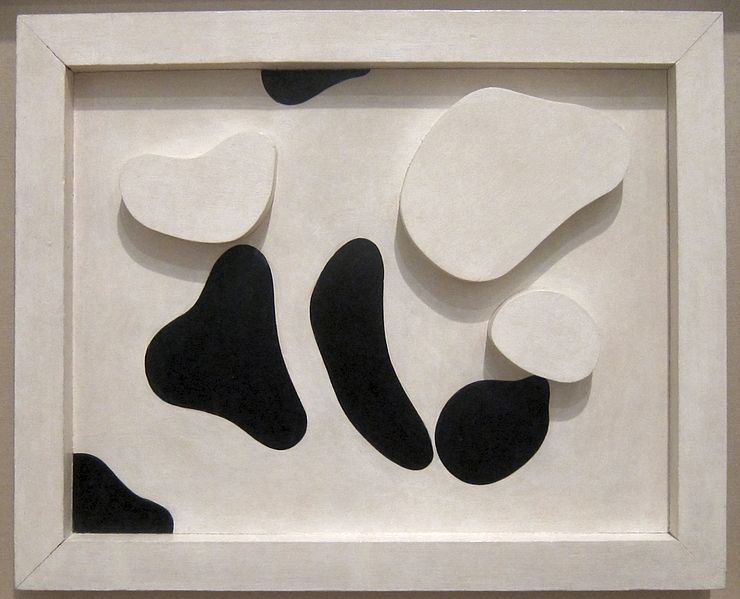
\includegraphics[width=5cm]{arp_hasard.jpg}
				\caption{Constellation selon les lois du hasard, Jean Arp, bois peint en relief, \textit{Tate Galleries}, Londres}
			\end{figure}
			
			Jean Clément dans \cite{clement2011} et Claire Labastie dans \cite{labastie2016} évoquent ces artistes précurseurs qui ont vu dans le fortuit, l'aléa, un point de départ pour la création. Claire Labastie met davantage l'accent sur la notion de sérendipité. La figure de Léonard de Vinci est notamment évoquée par ces deux auteurs. Selon Clément, Léonard aurait notamment mis en avant les tâches comme motif d'inspiration; et Labastie mentionne son génie primesautier, facteur de sérendipité et rendant propice la création. Plus proche de nous, mentions est faite de Strindberg, qui dans \textit{Du hasard dans la production artistique} \cite{strindberg1990} nous invitait à utiliser une guitare ``accordée au hasard'' ou un piano ``accordé au petit bonheur sans rime ni raison''.\\
					
			Et c'est de toute évidence ce qu'on fait les artistes au siècle suivant. Clément cite l'\textit{Erratum musical} de Marcel Duchamp \cite{duchamp1915}, une partition composée avec des notes tirées au hasard d'un chapeau. Il cite également Jean Arp et ses divers collages élaborés ``\textit{selon les lois du hasard}'' \cite{arp1916}, à l'aide de formes élémentaires (rectangles, patatoïdes...), collées à l'endroit même où elles sont tombées sur la toile. Nous pensons aussi bien sûr à Kandinsky et sa ``révélation'' face à l'une de ses oeuvre disposée à l'envers~:
			\begin{citationbox}
				\textit{[...] un tableau d'une indescriptible beauté, tout imprégné d'un flamboiement intérieur}
				\begin{flushright}
					Vassily Kandinsky, \textit{source inconnue}
				\end{flushright}
			\end{citationbox}
			Labastie fait aussi état des \textit{Frottages} de Max Ernst \cite{ernst1926}, une série de dessins résultats du ``frottage'' d'une mine de plomb sur un support en dessous duquel étaient placées de aspérités. Labastie évoque par ailleurs les ``trouvailles'' surréalistes, de simples objets ``élus'' par l'artiste selon les lois du ``hasard objectif''~:
			\begin{citationbox}
				\textit{À quelques boutiques de là, un choix presque aussi électif se porta sur moi sur une grande cuiller en bois, d'exécution paysanne, mais assez belle, me sembla-t-il, assez hardie de forme, dont le manche, lorsqu'elle reposait sur sa partie convexe, s'élevait de la hauteur d'un petit soulier faisant corps avec elle. Je l'emportais aussitôt.}\\
				\begin{flushright}
					André Breton, \textit{L'Amour fou}\cite{breton1937}
				\end{flushright}
			\end{citationbox}
			Ces objets sont pour André Breton les représentants de ce qu'il appelle une ``physique de la poésie''...\\
			
			Notons que nous sommes ici dans les arts au sens large : musique, peinture. Mais nous pensons que, d'une part les démarches d'artistes comme Duchamp ou Arp sont très semblables aux démarches des poètes combinatoires que nous étudierons plus loin dans l'exploitation d'un langage ``combinatoire discret'' (ensemble fini des notes de musique) ou simplement combinatoire (ensemble des formes en deux dimensions dont la taille est bornée par celle de la toile). De tels systèmes peuvent facilement être mis en relation avec le système des mots du langage, même si bien sûr les critères de correction sont sensiblement différents (plus permissifs en musique, et encore davantage en collage, par rapport aux critères grammaticaux et sémantiques du langage...). On note aussi la perte de contrôle de l'artiste dans ces jeux de hasard : une partie de l'acte de création est en quelque sorte déléguée à l'environnement, comme plus tard on déléguera une partie ou une totalité de la création à une machine. D'autre part, nous pensons comme Jean Clément que cette ouverture des arts au potentialités offertes par le hasard a remis en question une certaine conception de l'art en Occident, ce qui a par la suite ouvert la voie à une reconsidération de la littérature. Il est donc maintenant temps de nous intéresser aux premiers pas du hasard dans le domaine de la littérature.
		\subsection{Les surréalistes, cadavres exquis et écriture automatique}
			\subsubsection{Le cadavre exquis, une poétique à plusieurs}
				Le cadavre exquis est un jeu d'écriture collectif inventé par les surréalistes, en particulier Jacques Prévert et Yves Tanguy, vers 1925. Il s'agit sans doute de l'un des premiers exemples de littérature ``aléatoire''. L'aléatoire est dans ce cas précis ménagé par la pluralité des consciences qui produisent chacune indépendamment un fragment du poème ou de l'histoire finale (\textit{i.e.} un mot d'une classe grammaticale donnée \textit{a priori}). Des équivalents existent dans le monde anglo-saxon (\textit{round-robin stories}) et au Japon (\textit{Shiritori}).\\
				Cette méthode d'écriture n'est pas pleinement maîtrisée, car les paramètres liés aux choix des mots sont d'une part probabilistes, d'autre part fonction du co-auteur. Si l'on appelle $\mathbb{P}_k[i|j]$ la probabilité que le co-auteur n° $k$, devant choisir un mot dont la classe grammaticale est $j$, choisisse le mot $i$~:
				\begin{equation}
					\mathbb{P}_k[mot \ i' | classe \ j] \neq \mathbb{P}_k[mot \ i | classe \ j] \neq \mathbb{P}_{k'}[mot \ i | classe \ j]
				\end{equation}
				Cette méthode n'est pas non plus directement maîtrisée, dans la mesure où l'\textit{input} (la classe grammaticale) ne fixe que la syntaxe de l'\textit{output}, pas sa sémantique. Notons de surcroît que la sémantique des fragments produits par les co-auteurs n'est pas non plus nécessairement contrôlée par eux~: il suffit de penser au cas des mots polysémiques, comme chef, opéra, banc, anneau, souris... qui peuvent prendre un autre sens que celui attendu par leur producteur en fonction du contexte final.\\
				
				Car, plus généralement, la dernière source de variabilité dans la production réside dans l'harmonisation finale des productions. Cette harmonisation, que l'on pourrait très facilement comparer à un algorithme de consensus entre machines dans une architecture distribuée, peut consister selon les cas en un choix de genre, de nombre, de temps pour la phrase, et en quelques ajustement supplémentaires (prépositions...).\\
				
				\begin{figure}
					\begin{tabular}{c c}
						La pomme noir se transformer en l'ours euphorique & \\
						$\downarrow$ & [accord en genre non équivoque] \\
						La pomme noire se transformer en l'ours euphorique & \\
						$\downarrow$ & [accord en temps, équivoque]\\
						La pomme noire $\left\lbrace\begin{tabular}{l}
							se transforme en\\
							se transformera en\\
							se transformait en\\
						\end{tabular}\right.$
						l'ours euphorique & \\
						$\downarrow$ & [suppression d'article, équivoque]\\
						La pomme noire 
						$\left\lbrace\begin{tabular}{l}
							se transforme en\\
							se transformera en\\
							se transformait en\\
						\end{tabular}\right.$ ours euphorique & \\
					\end{tabular}
					\caption{Exemple d'un processus d'harmonisation après génération du cadavre exquis fragment par fragment par chaque co-auteur}
					\label{fig:consensus}
				\end{figure}
				
				Certains choix d'ajustement, comme le choix de supprimer un article défini (cf. Figure \ref{fig:consensus}), demeurent équivoques~: faut-il opter pour la bizarrerie (mais aussi la poésie) de la production originelle, ou normaliser le discours, possiblement à outrance~? Et à qui parmi les co-auteurs revient ce choix\footnote{on pourrait penser qu'il existe parmi les co-auteur un ``maître'' qui comme en calcul distribué s'occupe de passer les directives et de récupérer les résultats}? On voit par cet exemple que l'appréciation des auteurs intervient invariablement à la dernière étape, et d'une façon qui n'est pas forcément négligeable.\\
				
				L'harmonisation intervient en dernier ressort au niveau sémantique. Par exemple, dans un cadavre exquis comme ``Le banc -- attaqua -- la vase'', le syntagme ``le banc'' aura tendance à être interprété comme un banc de poissons (et non un banc public, acception pourtant plus fréquente), au vu du contexte (la vase rappelle le milieu aquatique).\\
				De même, dans un cadavre exquis comme ``L'anneau -- se transforma en -- corps'', les deux mots anneau et corps peuvent être vus comme des objets mathématiques (anneau et corps sont des types particuliers d'ensembles munis de lois spécifiques) ou bien être interprétés selon leurs acceptions communes (une alliance, et l'enveloppe charnelle d'un être). Dans ce cas, c'est la co-occurrence des deux mots anneau et corps qui peut évoquer l'interprétation mathématique, pourtant très peu fréquente et sans doute pas préméditée par les co-auteurs pris individuellement.\\
				
				Le cadavre exquis des surréalistes partage donc certains traits avec une littérature ``générative'', de par son architecture ``distribuée'' et son ``algorithme'' non-déterministe de consensus. La perte de contrôle sur le contenu provient de la pluralité des acteurs, et du caractère déphasé du consensus~: chacun choisit un mot indépendamment des autres, avec une mise en commun globale, impliquant des ajustements syntaxiques et des révisions sémantiques. Le résultat, aléatoire sans l'être tout à fait, peut donc être à la fois supérieur et différent de la somme de ses parties, ce qui fait la richesse de la méthode et son potentiel poétique.
				
			\subsubsection{\'{E}criture automatique, écriture robotique}\label{ecriture_auto}
				\begin{citationbox}
					\textit{Une telle beauté ne pourra se dégager que du sentiment poignant de la chose révélée, que de la certitude intégrale procurée par l'irruption d'une solution qui, en raison de sa nature même, ne pouvait nous parvenir par les voies logiques ordinaires. Il s'agit en pareil cas, en effet, d'une solution toujours excédante, d'une solution certes rigoureusement adaptée et pourtant très supérieure au besoin. L'image, telle qu'elle se produit dans l'écriture automatique, en a toujours constitué pour moi un exemple parfait.}
					\begin{flushright}
						André Breton, L'Amour fou, \cite{breton1937}
					\end{flushright}
				\end{citationbox}
				L'écriture automatique est perçue par les surréalistes comme une écriture de l'inconscient. Dans un état de demi-sommeil, les tabous sont levés et l'écrivain peut exprimer dans son œuvre son moi profond, le jaillissement de ses idées. L'écriture automatique est mentionnée par Claire Labastie dans \cite{labastie2016}. Elle parle notamment du recueil \textit{Les Champs magnétiques} (1924) \cite{breton1937}, écrit à deux mains par André Breton et Philippe Soupault~:
				\begin{citationbox}
					\textit{Les deux poètes
					transcrivent des mots dictés par l'inconscient, issus d'états semi-oniriques, qui arrivent
					spontanément de l'inconscient à la conscience.}
					\begin{flushright}
						Claire Labastie, \textit{Art, retard, hasard}\cite{labastie2016}
					\end{flushright}
				\end{citationbox}
				Le préfacier du recueil à sa première parution en 1968, Alain Jouffroy remarque aussi son caractère très avant-gardiste~:
				\begin{citationbox}
					\textit{Ils constituent, dans
					l’histoire de la littérature, le premier exemple d’écriture automatique, et
					répondent ainsi, cinq ans à l’avance, à la célèbre définition du
					surréalisme, telle qu’André Breton l’a formulée dans le premier
					manifeste de 1924~: ``Automatisme psychique pur par lequel on se
					propose d’exprimer soit verbalement, soit par écrit, soit de toute autre
					manière, le fonctionnement réel de la pensée.''.}\\
					Alain Jouffroy, \textit{Préface} pour \textit{Les Champs magnétiques}\cite{breton1968}
				\end{citationbox}
				
				Mais voir aujourd’hui l'écriture automatique comme une simple manifestation de l'inconscient, ce serait négliger (en partie tout au moins) la puissance du terme ``écriture automatique''. Car le choix de l'adjectif ``automatique'' en dit long~: une écriture \textit{automatique} est une écriture qui se fait toute seule, qui n'a plus besoin du secours de l'humain et de son intelligence rationnelle. Le terme ``automatique'' fait alors échos aux automates mécaniques comme ceux de Jaquet-Droz (cf. Figure \ref{fig:automate_jaquet_droz}). Cependant, même si ces marionnettes miment relativement bien l'acte d'écrire, on ne peut leur demander de produire spontanément du sens.\\
				
				Aujourd'hui, le terme d'écriture automatique prend une nouvelle signification. En effet, l'avènement des automates comme outils formels (cf. Section \ref{automates}) pour la génération de texte et la reconnaissance de langage donne une autre image de l'écriture ``automatique''. Un automate probabiliste à états finis (autrement dit, une chaîne de Markov, cf. Section \ref{markov}) fonctionne sur un système de transitions aléatoires d'un état vers un autre. Or, l'écriture automatique fonctionne également sur des associations d'idées locales et sur une liberté d'écriture qui favorise la sérendipité et les expressions fantaisistes mettant un point final au primat du sens. Nous pensons donc comme Jean-Pierre Balpe~:
				\begin{citationbox}
					\textit{elle est [la littérature générative], paradoxalement, beaucoup plus proche des dispositifs sous-tendant l'écriture surréaliste que de ceux sous-tendant une écriture réaliste dont elle paraît pourtant plus proche.}\\
					\begin{flushleft}
						Jean-Pierre Balpe, \textit{Un roman inachevé -- Dispositifs}\cite{balpe1994}
					\end{flushleft}
				\end{citationbox}
				Mais pour aller plus loin même que Jean-Pierre Balpe, nous pensons que l'on pourrait établir des liens entre l'écriture automatique des surréalistes et une écriture automatique éminemment moderne~: celle des claviers de smartphone. En effet, il est très facile de générer du texte à partir des suggestions d'un clavier d'Android. Ces suggestions dépendent du contexte (mots déjà écrits), et des statistiques passées sur l'usage et la fréquence des mots. Ainsi, on pourrait voir le texte généré par un clavier d'Android comme une manifestation des préoccupations plus ou moins profondes de l'utilisateur du téléphone. Une ``illustration'' de cette hypothèse est donnée en Annexe \ref{android}. Le texte est généré à partir du smartphone de l'auteure de ce mémoire, et semble évoquer ses problèmes de recherche de stage (à noter les nombreuses formules de politesse liées aux mails envoyés \textit{via} le téléphone), des aspects de sa vie privée (nom de connaissances proches...), et des éléments relatifs à son lieu de vie (stations de métro parisiennes...). Le texte est globalement plus cryptique que les textes surréalistes, mais nous pensons que l'esprit demeure le même.\\
				
				En plus d'anéantir la sémantique au sens strict, l'écriture automatique brise parfois les codes sociaux et moraux, à l'instar d'une machine insoucieuse de la bienséance. Cela est souligné par Labastie~:
				\begin{citationbox}
					\textit{Par la rapidité entre la survenue des mots et leur transcription, les poètes prennent de vitesse le désir de rationalité, l'empêchent d'annuler les images absurdes ou choquantes.}
					\begin{flushright}
						Claire Labastie, \textit{Art, retard, hasard}\cite{labastie2016}
					\end{flushright}
				\end{citationbox}
				
				L'écriture automatique se rapproche donc de la littérature générative selon l'angle du processus (par transitions aléatoires d'un état à un autre) et selon l'angle du contenu (libéré des contraintes sémantiques et morales). Toutefois, Labastie souligne l'existence d'un contrôle résiduel de l'auteur qui nous le verrons sera un constante des premiers travaux en matière de littérature générative\footnote{on retrouve ce contrôle chez Lutz, dans l'OuLiPo, dans le cas du robot Calliope évidemment...}.
				\begin{citationbox}
					\textit{Après-coup, dans un deuxième temps, les images, les mots étant apparus et transcrits, les poètes en élaguent probablement des parties jugées faibles et en en réarrangent sommairement les autres, tout en conservant le pouvoir poétique des images impromptues sorties de l'inconscient}
					\begin{flushright}
						Claire Labastie, \textit{Art, retard, hasard}\cite{labastie2016}
					\end{flushright}
				\end{citationbox}
				
		\subsection{Les ``poètes programmeurs''}
			\subsubsection{Les \textit{Lettres d'amour} (\textit{Love Letters}) de Christopher Strachey}
				Les ``Lettres d'amour'' (\textit{Love Letters}) de Christopher Strachey furent créées en 1952. Ces lettres sont le résultat d'un algorithme combinatoire que Strachey avait développé pour le Manchester Mark 1 (cf Figure \ref{fig:manchester_mark_1}), l'un des premiers ordinateurs électroniques, développé comme son nom l'indique à l'Université de Manchester. Les poèmes d'amour de Strachey sont vus comme les premiers exemples de littérature informatique. Il étaient à l'époque produits sous forme imprimée, du fait notamment de l'absence d'interfaces graphiques poussées.
				
				\begin{figure}
					\centering
					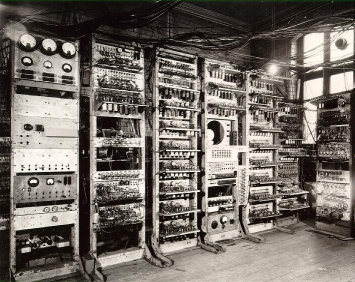
\includegraphics[width=5cm]{manchester_mark_1.jpg}
					\caption{Ordinateur Manchester Mark 1, photographie prise en 1949. Copyright~: Université de Manchester.}
					\label{fig:manchester_mark_1}
				\end{figure}
				Ces lettres s'appuyaient sur une structure ``narrative'' fixe~:
				\vspace{2mm}
				\begin{itemize}
					\item une phrase de salutation
					\item cinq phrases pour le corps du texte
					\item une phrase de clôture, signée M.U.C (pour Manchester University Computer (!))
				\end{itemize}
				\vspace{2mm}
				Les phrases composant le corps du texte possédaient elles-aussi une structure syntaxique fixe, et pouvaient être de deux types différents (une longue ou une plus courte), possiblement coordonnées. En revanche, les mots composant les phrases étaient tirés au hasard dans différents sous-ensembles de mots (noms, verbes, adjectifs, adverbes), selon le principe dit des ``moules'' ou encore des ``phrases à trou''.  La liste des mots ``candidats'' de chaque sous-ensemble a été compilée par Strachey sur la base du Thésaurus de Roget \cite{wiki:roget}.\\
				
				Compte tenu de la taille des différents sous-ensembles de mots et des règles de combinaison, l'algorithme de Strachey, malgré sa grande simplicité, était en mesure  de produire près de 318 000 milliards de lettres différentes.  Nous sommes donc ici dans un exemple canonique de génération combinatoire (finie). Philippe Bootz dans \cite{bootz} ne manque pas de remarquer le caractère assez rudimentaire du dispositif, ainsi que la faible importance du style et de la portée littéraire des productions. Mais sans doute était-ce là un parti pris, dans l'optique de mettre en valeur le contraste significatif entre la simplicité des instructions et la multiplicité des productions possibles, mais aussi  peut-être d'un point de vue plus littéraire, le caractère très stéréotypé de l'amour hétéronormé (critique \textit{queer}...).\\
				
				En ce sens, Christopher Strachey semble annoncer une vision de l'ordinateur comme outil de critique littéraire et sociale.
		
			\subsubsection{Theo Lutz et les \textit{Textes Stochastiques} (\textit{Stochaschische Texte})}
				Theo Lutz (1932-2010) était un informaticien allemand et un élève du philosophe Max Bense. Il était de fait proche de l'école de Stuttgart, qui cherchait à promouvoir la littérature expérimentale et l'art.  Il  est considéré, au travers de ses \textit{Textes Stochastiques} notamment, comme pionnier dans le domaine de la poésie numérique. Ces \textit{Textes Stochastiques}, que Theo Lutz a créés en 1959 à Stuttgart en programmant un algorithme pour un Z22\footnote{le Z22 est un ordinateur qui fut développé en 1955 par le physicien Lorenz Hanewinkel pour le compte l'entreprise Zuse KG (Konrad Zuse). Le Z22 fut le premier ordinateur à tube de l'Allemagne de l'Ouest.} conçu par Konrad Zuse, sont en effet considérés comme les premiers poèmes générés par ordinateur :
				\begin{citationbox}
					\textit{Le générateur de Lutz est donc très proche, dans sa présentation, de ceux qui l'ont précédé. Et pourtant cette publication est souvent considérée comme l'acte de naissance de la poésie numérique et, par-là même, de la littérature numérique.}
					\begin{flushright}
						Philippe Bootz, \textit{Un historique de la génération numérique de textes}\cite{bootz}
					\end{flushright}
				\end{citationbox}
				Philippe Bootz justifie ce point de vue par les modalités de publication des \textit{Textes Stochastiques}~:
				
				\begin{citationbox}
					\textit{Indeed, publishing generated poems in a review of avant-garde literature is more engaged from a literary standpoint than programming of letters by engineers.}
					\begin{flushright}
						Philippe Bootz, \textit{From OULIPO to Transitoire Observable} \cite{bootz2012}
					\end{flushright}
				\end{citationbox}
				
				L'algorithme des \textit{Textes Stochastiques}, comme le précise Philippe Bootz, est très proche de l'algorithme de Strachey : tous deux reposent sur le principe du ``moule'', ou des ``phrases à trous'', et sur une présentation au format imprimé (\textit{teleprinter}, pas d'écran).\\ L'expérimentateur entre une série de noms communs en précisant leur genre (en allemand, féminin, masculin ou neutre), ainsi qu'une série d'adjectifs. Dans la version originale de l'algorithme, 16 noms et 16 adjectifs avaient été sélectionnés à partir du \textit{Château} de Franz Kafka (la liste est fournie en Annexe \ref{stochastische_texte_algo}).\\
				L'algorithme va ensuite choisir un ``moule'' parmi une liste finie préprogrammée, et ``remplir'' ce moule avec les noms et adjectifs passés en argument et tirés au hasard à la volée. Chaque ``moule'' engendre alors une (ou deux\footnote{le moule est en effet la coordination de deux ``sous-moules''. La coordination peut s'opérer à l'aide de conjonctions, auquel cas on obtient bien une seule phrase, ou à l'aide d'un point, auquel cas on obtient deux phrases séparées.}) phrase courte, qui ressemble de par sa formulation à une maxime (un [nom] est [adjectif], tout [nom] est [adjectif]...).\\
				Nous avons pris le soin de retranscrire le principe de remplissage des ``moules'' sous la forme d'une grammaire générative, en Annexe \ref{stochastische_texte_algo}. Il est par ailleurs possible de tester librement l'algorithme (avec ses données d'origine) sur cette page : \href{https://auer.netzliteratur.net/0_lutz/lutz_original.html}{https://auer.netzliteratur.net/0\_lutz/lutz\_original.html}.\\
				
				En ce qui concerne la publication et la réception de l'œuvre de Theo Lutz, l'algorithme des \textit{Textes Stochastiques} ainsi que 35 résultats d'exécution (donc 35 phrases ou doubles phrases) sur 50 essais au total ont été publiés en 1959 dans la revue \cite{lutz1959} \textit{Augenblick} (traduit de l'allemand à l'anglais par Helen MacCormac, 2005 ici : \href{http://www.stuttgarter-schule.de/lutz_schule_en.htm}{http://www.stuttgarter-schule.de/lutz\_schule\_en.htm}). Notons qu'il s'agit là d'un sous-ensemble minime de toutes les productions possibles, en effet, le nombre total de possibilités est donné par : 
				\begin{eqnarray*}
					[N_{Noms} \times N_{adjectifs} \times N_{Phrases}]^2 \times N_{conjonctions} &=& [16 \times 16 \times 4]^2 \times 4\\
					&=& 1024^2 \times 4\\
					&=& 41943041 \footnotemark \\
				\end{eqnarray*}	
				\footnotetext{à noter que l'article original contient une coquille, le résultat de $1024^2*4$ est bien 4194304 et non 4174304 comme indiqué.}
				Dans cet article, Theo Lutz semble d'abord adopter un point de vue utilitariste (que  l'on pourrait qualifier de point de vue ``d'ingénieur''). Il met en avant les avantages de sa méthode en termes d'efficience et de rapidité plutôt qu'en termes de créativité, de teneur poétique :
				\begin{citationbox}
					\textit{Our program's task was to take over the laborious production of stochastic texts. In the past such texts were determined by selecting sentences or constituents of a sentence by throwing dice, or using some other random process, and then connecting these. It seemed reasonable for the program-controlled data processor to work with so-called random numbers, as a stochastic process.}
					\begin{flushright}
						Theo Lutz, \textit{Stochastische Texte}, traduction Helen MacCormac \cite{lutz1959}
					\end{flushright}
				\end{citationbox}
				Les \textit{Textes Stochastiques} sont donc davantage perçus comme un moyen plus efficace et moins ``laborieux'' de générer du contenu textuel aléatoire, sans réelle avancée esthétique.\\
				
				En revanche, là où les \textit{Textes Stochastiques} vont plus loin comparés aux poèmes de Strachey, c'est dans les perspectives qu'ils ouvrent. Theo Lutz évoque en effet à la fin de son article dans \textit{Augenblick} ce qui serait aujourd’hui qualifié de \textit{machine learning} basique :
				\vspace{2mm}
				\begin{itemize}
					\item imitation de style : il serait possible de modifier le \textit{prior} de l'algorithme (c'est-à-dire la distribution de probabilité des mots, qui par défaut est une loi uniforme), afin d'imiter le style d'un auteur. Par exemple, on pourrait assigner au mot gouffre'' une probabilité plus grande et au mot ``joie'' une probabilité plus faible en vue ``d'imiter'' un poème de Baudelaire.
					\item cohérence sémantique :  il serait possible d'introduire des probabilités jointes (sous forme matricielle) pour les noms et les adjectifs (les tirages ne seraient donc plus indépendants), ceci dans le but de favoriser certaines associations ayant plus de pertinence sémantique\footnotemark. Par exemple, la probabilité de tirer ``incolore'' après ``idées'' devrait être plus faible que la probabilité de tirer ``géniales'', et inversement, ``incolore'' sera plus probable que ``géniale'' après avoir tiré ``substance'' 
				\end{itemize}
				\vspace{2mm}
				\footnotetext{ce genre de procédé est encore tout à fait d'actualité ! De nos jours, la matrice de probabilités est estimée à l'aide de données statistiques de co-occurrence des mots au sein de corpus massifs de texte. Cela est utilisé en génération de texte évidemment (la co-occurrence peut-être étendue à une fenêtre de taille donnée, et on applique à la matrice ainsi obtenue une décomposition en valeurs singulières qui renvoie une représentation vectorielle des mots...), mais aussi dans les moteurs de recherches (algorithme TF-IDF) afin de mesurer la pertinence d'un page web par rapport à une requête donnée !}
				
				Notons d'ailleurs (mais cela n'est pas explicitement souligné par Theo Lutz), que les deux phénomènes peuvent se conjuguer. Par exemple, si ``gouffre'' est choisi comme nom et que l'on cherche de plus à imiter un poème de Baudelaire, la probabilité de tirer ``amer'' comme adjectif sera augmentée. En ce sens, l'algorithme de Theo Lutz peut réellement être vu comme un point de départ pour des méthodes plus élaborées, à l'origine de nos algorithmes statistiques actuels (cf. Section \ref{methodes_stat}).
		\subsection{Les collectifs~: OuLiPo, ALAMO}
			\subsubsection{L'OuLiPo}
				Les ``jeux littéraires'' développés par les surréalistes trouvèrent leur continuation dans les travaux de l'OuLiPo (\textbf{Ou}vroir de \textbf{Li}ttérature \textbf{Po}tentielle), un groupe formé de littéraires et de mathématiciens se définissant eux-mêmes comme des ``rats qui construisent eux-mêmes le labyrinthe dont ils se proposent de sortir''. Nous détaillerons quelques uns des exemples les plus marquants liés à ce groupe, une liste plus exhaustive des ``contraintes'' pouvant être trouvée sur \href{http://oulipo.net/fr/contraintes}{http://oulipo.net/fr/contraintes}\footnote{on conseille d'ailleurs de lire cette section dans sa version numérique, car chaque contrainte mentionnée est associée à un lien hypertexte vers son énoncé plus complet présent sur le site de l'OuLiPo.}.
				\begin{citationbox}
					\textit{Les écritures à contrainte sont souvent mobilisées, très logiquement, puisqu’elles furent produites au sein de cadres formels qui ne sont pas sans rappeler les cahiers des charges imposés à la création numérique par les ``architextes'', ces outils au service d’une énonciation éditoriale.}\begin{flushright}
						Gilles Bonnet, \textit{Le livre implémenté} \cite{bonnet2017}
					\end{flushright}
				\end{citationbox}
				
				Nous allons voir que dans ce groupe, la dimension algorithmique est aussi bien plus marquée, même si l'aspect davantage computationnel (utilisation d'ordinateurs, programmation) fut longtemps négligé.\\
				
				Dans notre présentation des jeux littéraires de l'OuLiPo, nous nous appuierons sur une typologie tirée de la programmation et de la logique. Un programme informatique peut être modélisé comme un triplet de Hoare~: {P}C{Q} où P et Q sont des \textit{prédicats} (respectivement préconditions et postconditions) et où C est un \textit{programme}, c'est à dire un suite d'instructions. Nous allons voir que les jeux oulipiens se classifient aisément suivant ces trois composantes, selon qu'ils mettent l'accent sur les préconditions (les éléments à utiliser, à combiner), le programme (aspect algorithmique, procédural de la création) ou les postconditions (création dans le respect constant des contraintes finales).
				
				\subsubsubsection{Les jeux combinatoires}
					Les jeux combinatoires sont les jeux mettant en avant le ``domaine'' (l'ensemble des briques constitutives) de la création. Cet ensemble est bien souvent restreint et contraignant, ce qui pousse à en explorer toutes les combinaisons, d'où l'appellation de jeux combinatoires. Le domaine du jeu peut bien sûr varier dans sa nature~: il peut être constitué de lettres à recombiner (les lettres les plus courantes de l'alphabet dans \href{http://oulipo.net/fr/contraintes/onzain-heterogrammatique}{``Onzain hétérogrammatique''} et \href{http://oulipo.net/fr/contraintes/ulcerations}{``Ulcérations''}, les lettres d'un prénom dans \href{http://oulipo.net/fr/contraintes/beau-present}{``Beau présent''}), de mots (\href{http://oulipo.net/fr/contraintes/aphorisme}{``Aphorisme''}), ou de phrases (vues au sens mathématique comme des suites de mots, on pense par exemple aux 14 vers composant une instance de \href{http://oulipo.net/fr/contraintes/cmmp}{``CMMP''}\footnote{notons cela dit que le cas de CMMP est un peu différent~: l'aspect combinatoire du poème ne se fait jour qu'au moment de l'``instanciation'', c'est-à-dire quand le lecteur feuillette les livre. L'auteur lui, avait tout latitude dans le choix de ses mots et de ses phrases. Le lecteur lui, ne peut plus changer les vers à combiner, ils constituent donc le ``domaine'' restreint de son jeu.}).\\
				
					Par ailleurs, l'aspect combinatoire varie selon les jeux~: il peut être plus ou moins contrôlé selon les cas. Certains jeux comme ``CMMP'' tendent à explorer toutes les combinaisons possibles\footnote{dans l'absolu tout du moins, car ouvrir et fermer le livre au hasard plus d'un millions prendrait des jours entiers}, sans préférence. D'autres jeux comme ``Beau présent'', ``Onzains hétérogrammatiques'', ``Ulcérations'' orientent le choix des combinaisons possibles en vue d'une correction lexicale et syntaxique. On pourra dire qu'en général, plus le domaine est atomique (les lettres sont plus atomiques que les mots qui sont plus atomiques que les phrases qui sont plus atomiques que les récits, les poèmes etc.), plus la combinatoire sera orientée, car les contraintes de correction et d'intelligibilité se font plus pressantes.
				
					%Hasard, Aphorisme, Beau présent, CMMP, Onzain hétérogrammatiques, Ulcérations
					
					\begin{citationbox}
						\textit{Plus qu'un texte, parmi la quasi infinité d'instanciations possibles qu'il ouvre -- rien effectivement ne
					légitimera telle réalisation particulière plutôt que telle autre, toutes valent
					également ensemble, voire encore, aucune ne vaut par elle-même -- le
					générateur combinatoire offre une mise en œuvre de la transformation
					(réglée ou aléatoire, peu importe ici) de ses variantes successives [...]}
					\begin{flushright}
						Ambroise Barras, \textit{Prolégomènes à toute littérature informatique} \cite{barras1995}
					\end{flushright}
					\end{citationbox}
				
				\subsubsubsection{Les jeux algorithmiques}
					Les jeux algorithmiques mettent l'accent sur la procédure, le programme à suivre, qui devient quasiment plus important que le résultat final, du moins dans l'acception ``potentielle'' de la littérature que défend l'OuLiPo. Les ``algorithmes'' présents dans les contraintes oulipiennes reprennent des aspects divers de la programmation~:
					\vspace{2mm}
					\begin{itemize}
						\item la compression, avec \href{http://oulipo.net/fr/contraintes/anaerobie}{``Anaérobie''}, \href{http://oulipo.net/fr/contraintes/bord-de-poeme}{``Bord de poème''} pour une compression directe, \href{http://oulipo.net/fr/contraintes/algorithme-de-mathews}{``Algorithme de Mathews''} qui étonnamment préfigure un ``vrai'' algorithme de compression, BWT, inventé en 1994 et encore utilisé en génomique~!;
						\item l'utilisation ou le parcours de structures de données classiques comme les graphes, avec \href{http://oulipo.net/fr/contraintes/graphe}{``Graphe''} ou les arbres, avec \href{http://oulipo.net/fr/contraintes/conte-a-votre-facon}{``Conte à votre façon''}, \href{http://oulipo.net/fr/contraintes/tireur-a-la-ligne}{``Tireur à la ligne''};
						\item tout un travail sur les chaînes de caractères, que ce soit du \textit{parsing} ou des substitutions au niveau syntaxique avec \href{http://oulipo.net/fr/contraintes/chimere}{``Chimère''}, au niveau lexical avec \href{http://oulipo.net/fr/contraintes/transduction}{``Transduction''}, ou au niveau sémantique avec \href{http://oulipo.net/fr/contraintes/litterature-definitionnelle}{``Littérature définitionnelle''} et \href{http://oulipo.net/fr/contraintes/lsd}{``LSD''} qui au passage se rapprochent de l'\textit{inlining} en compilation...,
						\item la cryptographie avec \href{http://oulipo.net/fr/contraintes/s7}{``S+7''} et \href{http://oulipo.net/fr/contraintes/sde}{``S+dé''} qui s'apparentent à des codes César.
					\end{itemize}
					\vspace{2mm}
					Tous ces jeux algorithmiques sont plus ou moins sensibles à l'\textit{input}, donc plus ou moins robustes. Encore un fois, les algorithmes manipulant des caractères (comme ``l'Algorithme de Mathews'', ``Anaérobie'') sont moins robustes que les algorithmes manipulant des mots (``Transduction'', ``LSD'', ``S+7''), qui sont eux-mêmes moins robustes que les algorithmes manipulant des phrases (``Conte à votre façon'').\\
					Par conséquent, lorsqu'il s'agit de créer des résultats surprenants et lorsque l'algorithme est relativement cryptique (complexe comme ``l'Algorithme de Mathews'', ou arbitraire comme ``Anaérobie''), le choix de l'\textit{input} est important, et l'on rejoint la catégorie des jeux combinatoires.
				
					%Mathews, Anaérobie Bord de vers Chimère Conte à votre façon Graphe Littérature définitionnelle LSD Transduction Tireur à la ligne S+7 S+dé
				
				\subsubsubsection{Les jeux à contraintes}
					Même si l'OuLiPo appelle tous ses jeux ``contraintes'', certains jeux sont plus axés sur les règles que d'autres. De tels jeux pourraient se résumer ainsi~: faites ce que bon vous semble tant que le produit final satisfait un certain nombres de critères additionnels de correction (en plus des critères classiques d'orthographe, de grammaire etc.). Ces jeux sont en général plus orientés vers les mathématiques que l'informatique pure. On pourrait découper les contraintes en deux catégories~:
					\vspace{2mm}
					\begin{itemize}
						\item les contraintes formelles dans le respect de certains \textit{patterns} de caractères (\href{http://oulipo.net/fr/contraintes/palindrome}{``Palindrome''} qui est très lié à la théorie des automates, cf. \ref{automates}, \href{http://oulipo.net/fr/contraintes/avion}{``Avion''} qui reprend des idées de compression) ou de mots (\href{http://oulipo.net/fr/contraintes/cylindre}{``Cylindre''} qui reprend des idées de la topologie quotient, \href{http://oulipo.net/fr/contraintes/cylindre}{``Boule de neige''}), de certaines règles de transformation sur les caractères (\href{http://oulipo.net/fr/contraintes/facteur-commun-mise-en}{``Facteur commun (mise en)''}, qui s'inspire du calcul), 	ou de contraintes mixtes caractères/mots ou mots/phrases (\href{http://oulipo.net/fr/contraintes/desarguesienne}{``Désarguesienne''} qui s'inspire de la géométrie).
						\item les contraintes sémantiques inspirées de la géométrie (\href{http://oulipo.net/fr/contraintes/contrainte-de-pascal}{``Contrainte de Pascal''}), ou de l'analyse (principe de compositionnalité sémantique ``à la sauce Fibonacci'' dans \href{http://oulipo.net/fr/contraintes/hypertropes}{``Hypertropes''})
						\item un mixte des deux, selon un principe réflexif (\href{http://oulipo.net/fr/contraintes/villanelle}{``Villanelle''}, qui explique une contrainte tout en l'appliquant, \href{http://oulipo.net/fr/contraintes/portrait-en-creux}{``Portrait en creux''} où typographie et style définissent leur objet par négation).
					\end{itemize}
					\vspace{2mm}
					Les jeux à contraintes sont bien évidemment très proches des jeux algorithmiques, dans la mesure ou se donner une contraintes, c'est aussi se donner une méthode pour la respecter. 
				
				
				
	%Palinfrome => formel
	%Avion =>formel
	%Boule de neige => formel
	%Cylindre => formel
	%Déarguésienne => formel
	%Facteur commun => forme
	%Hypertropes => fond
	%Portrait en cruex => forme et fond
	%Villanelle => fond et forme
	%Contrainte de pascal => fond
				
				\subsubsubsection{Synthèse}
					Nous avons dans cette présentation non exhaustive des contraintes oulipiennes privilégié les jeux les plus proches des mathématiques et de la logique, explorant des théories mathématiques relativement poussées (Théorème de Desargues, Théorème de Pascal, suites numériques), mais aussi les fondements de l'informatique (théorie des automates et des transducteurs, lambda-calcul et substitutions). Mais l'OuLiPo fut aussi à l'origine de jeux plus littéraires, en particulier un bon nombre de formes poétiques. Cela dit, nous avons pu constater que le fragment des contraintes oulipiennes que nous avons choisi d'étudier se répartit de façon harmonieuse entre les différentes composantes d'un programme informatique (préconditions, instructions, postconditions), ce qui tend à montrer que l'Oulipo s'appuie sur des aspects fondamentaux de l'informatique. Cela dit, force est de constater qu'aucune des contraintes évoquées ne satisfait réellement aux trois critères, malgré des efforts de présentation qui font des énoncés de contraintes une partie de l'œuvre elle-même (notamment dans ``Anaérobie'' et ``Beau présent''). Les contraintes oulipiennes ne pourraient donc être qualifiées d'algorithmes bien-formés. Et ce n'était sans doute pas le but, car il s'agissait avant tout de jouer avec les mots, et de conserver la figure de l'auteur comme figure créatrice.
				
					\begin{citationbox}
						\textit{Il est cependant nécessaire d'ajouter que si les membres de l'OuLiPo manifestaient la volonté de techniciser la littérature et d'utiliser des machines pour traiter l‘information, ils n'ont jamais vraiment remis en cause les notions d'œuvre littéraire, et encore moins de littérature.}
						\begin{flushright}
							Anaïs Guilet et Franck Soudan, \textit{Robopoïèse}\cite{guilet2017}
						\end{flushright}
					\end{citationbox}
					
					Du reste comme le précise Philippe Bootz, l'OuLiPo ne s'est penché sur la programmation informatique des contraintes que très tard, en 1975~:
					\begin{citationbox}
						\textit{However, the OULIPO came late to actual computational practice, in 1975, when Paul Braffort programmed the Cent mille milliards de poèmes for the Europalia exhibition to Brussels.\\
						Several years after this exhibition, the OULIPO considered that the relationship between literature and computer science was a specific topic.}
						\begin{flushright}
							Philippe Bootz, \textit{From OULIPO to Transitoire Observable} \cite{bootz2012}
						\end{flushright}
					\end{citationbox}
					C'est en fait un autre groupe ``consanguin'' de l'OuLiPo qui reprendra le flambeau de l'informatisation. Il s'agit de l'ALAMO, dont nous allons discuter dans la section suivante.
				
%				OuLiPo, un mouvement anti-hasard... Au contraire de max bense. À propos de son roman La Vie mode d'emploi (1978), Georges Perec parlait cependant d'``aléatoire mécanique'' et de ``programmation du hasard''~: d'une littérature stochastique, en quelque sorte. ``Il n'y a de littérature que volontaire'', écrivait Raymond Queneau [Oulipo, 1973~: 27])
				
				
%				appeler la dichotomie entre programmation impérative et programmation par contraintes
			\subsubsection{L'ALAMO}
				Comme nous l'avons vu, L'OuLiPo s'est intéressé à la relation entre la littérature et l'informatique selon un point de vue algorithmique et combinatoire, sans passer par l'étape obligée de l'implémentation. L'ALAMO (\textbf{A}telier de \textbf{L}ittérature \textbf{A}ssistée par la \textbf{M}athématique et les \textbf{O}rdinateurs) s'est formé en 1981 afin de répondre à ce manque, mais aussi afin d'éviter une confusion des approches chez le public (combinatoire pour l'OuLiPo, informatique pour l'ALAMO) \cite{alamo}.\\
				
				L'ALAMO a été fondé par Paul Braffort et Jacques Roubaud, deux membres de l'OuLiPo. le groupe comptait à ses débuts neuf membres, dont quatre oulipiens (les deux fondateurs, plus Marcel Bénabou et Paul Fournel), et cinq non oulipiens (en particulier Jean-Pierre Balpe sur lequel nous reviendrons Section \ref{balpe}). En 2008, l'ALAMO était encore formé de $17$ membres. Comme le précise Philippe Bootz dans \cite{bootz2012}, l'ALAMO ne s'est pas autant développé que l'OuLiPo, mais est resté relativement stable autour du même cercle d'écrivains (mis à part le départ de Jean-Pierre Balpe notamment). De plus, le groupe a pu bénéficier d'aides de l'État pour organiser des rencontres autour du thème de la littérature informatique (notamment, l'exposition des \textit{Immatériaux} an centre Pompidou en 1985). Les objectifs de l'ALAMO \cite{alamo} sont~:
				\vspace{2mm}
				\begin{itemize}
					\item la génération automatique de textes littéraires, étant données certaines contraintes (en fait nous verrons qu'il s'agit souvent d'une remédiatisation de contraintes oulipiennes ou de leurs variantes);
					\item le développement d'outils informatiques à l'usage des écrivains, pour générer leurs propres œuvres;
					\item la formation et la pédagogie autour de l'ordinateur et de la littérature
				\end{itemize}
				\vspace{2mm}
				Dans ce qui suit, nous nous concentrerons sur les deux premiers points qui touchent plus directement à la littérature générative, et nous délaisserons donc le côté ``Atelier'' de l'ALAMO.
				\subsubsubsection{Programmes génératifs}
					Nous ne nous étendrons pas sur cette section, car l'esprit derrière les programmes génératifs de l'ALAMO est -- il faut le dire -- sensiblement le même que celui de l'OuLiPo. Certains programmes de l'ALAMO sont en effet des remédiatisations des contraintes oulipiennes, notamment les programme des ``Aphorismes'' (\href{http://oulipo.net/fr/contraintes/aphorisme}{version OuLiPo}, \href{http://www.alamo.free.fr/pmwiki.php?n=Programmes.Aphorismes}{version ALAMO}) et des ``Locutions introuvables'' (\href{http://oulipo.net/fr/contraintes/locutions-introuvables}{version OuLiPo}, \href{http://www.alamo.free.fr/pmwiki.php?n=Programmes.LocutionsIntrouvables}{version ALAMO}).\\
					D'autres programmes sont l'adaptation de contraintes oulipiennes à des corpus différents, notamment \href{http://www.alamo.free.fr/pmwiki.php?n=Programmes.Rimbaudelaires}{``Rimbaudelaires''} (qui est une variété de \href{http://oulipo.net/fr/contraintes/chimere}{``Chimère''} avec comme moule \textit{Le Dormeur du val} et comme base lexicale le vocabulaire baudelairien) et \href{http://www.alamo.free.fr/pmwiki.php?n=Programmes.Triolets}{``Triolets de Braffort''} (même principe que \href{http://oulipo.net/fr/contraintes/cmmp}{``CMMP''}, mais une forme différente, celle du triolet).\\
					Certains programmes de l'ALAMO semblent accorder plus de place au corpus, et usent en particulier de textes littéraires~: \href{http://www.alamo.free.fr/pmwiki.php?n=Programmes.AlexandrinsAuGreffoir}{``Alexandrins au greffoir''} mélange les hémistiches d'alexandrins célèbres (Ronsard, Hugo, Mallarmé...), \href{http://www.alamo.free.fr/pmwiki.php?n=Programmes.BaiserDeKuhlman}{``Les Baisers d'Amour de Quirinus Kuhlmann''} reprend comme ``moule'' le XLI$^{eme}$ \textit{Baiser} de Kuhlmann, les \href{http://www.alamo.free.fr/pmwiki.php?n=Programmes.LitaniesDeLaVierge}{``Litanies de la Vierge''} recomposent les hémistiches du poème du même nom écrit Jean Meschinot (1415-1491).\\
					
					Pour nous, les programmes de l'ALAMO présentent donc trois avancées ou différences par rapport aux jeux de l'OuLiPo~:
					\vspace{2mm}
					\begin{itemize}
						\item comme on l'a dit, un intérêt pour les corpus littéraires, et donc pour le pastiche de style (que l'on retrouve dans les programmes actuels, cf. notre petite simulation sur des poèmes de Hugo avec un réseau de neurones Section \ref{lstm_hugo});
						\item une internalisation des contraintes au niveau du programmes, contraintes spécifiques au jeu, mais aussi plus généralement contraintes phonétiques, prosodiques, rythmiques, syntaxiques, sémantiques... ces derniers types de contraintes faisaient l'objet d'un ajustement humain non-systématisé du temps de l'OuLiPo;
						\item la possibilité d'expérimenter en ligne et instantanément les différentes combinaisons (à voir sur le site officiel de l'ALAMO).
					\end{itemize}
				\subsubsubsection{Des outils pour l'écrivain}
					\begin{citationbox}
						\textit{Par ailleurs, il devenait évident que la mise au point d'algorithmes réellement interactifs ``intelligents'', c’est-à-dire permettant à l’utilisateur de créer lui-même un programme de création nous obligeait à concevoir, une méthodologie nouvelle, de niveau supérieur~: un véritable} langage-auteur.
						\begin{flushright}
							\textit{Site officiel de l'ALAMO} \cite{alamo}
						\end{flushright}
					\end{citationbox}
					Cette sous-section est consacrée à un aspect un peu ``méta-'' de la littérature générative, puisque l'ALAMO s'est proposé de créer des interfaces pour générer des textes littéraires. Baptisés \textit{littéraciels}, ces outils ont été développés au milieu des années 80. Les premiers littéraciels visaient des domaines textuels très précis, et souvent très stéréotypes~: petites annonces matrimoniales (projet SEL(TS)), textes dramatiques (projet SCENARIO). Plus tard, la démarche a été généralisée au sein du projet LAPAL (littéraciel conçu et réalisé par Anne Dicky). Les littéraciels se fondent sur trois paramètres ajustables par l'écrivain qui les utilise~:
					\vspace{2mm}
					\begin{itemize}
						\item un ensemble de départ composé d'éléments textuels issus de lexiques variés mais prédéfinis;
						\item un ensemble de ``moules'' plus ou moins complexes et plus ou moins spécifiés, pouvant prendre la forme de phrases à trous (très spécifiées), ou d'arbres syntaxiques (plus abstraits, cf. Section \ref{grammaires} pour des exemples plus précis);
						\item un ensemble de contraintes littéraires réduisant le champ des possibles, c'est-à-dire le nombre de combinaisons réalisables.
					\end{itemize}
					\vspace{2mm}
					Il s'agit là d'un modèle abstrait, d'un genre de cahier des charges. A ces \textit{desiderata} correspondent des structures informatiques ``réelles'' et nécessaires à l'implémentation du projet~:
					\vspace{2mm}
					\begin{itemize}
						\item un arbre syntaxique spécifie la composition du texte. Les \textit{feuilles} de l'arbre décrivent la nature des éléments lexicaux tandis que les \textit{nœuds internes} détaillent comment ces éléments sont combinés étape par étape. La notion d'élément lexical est élargie et va de la notion de mot à celle de paragraphe entier;
						\item une ``déclaration de subordination'' permet de formaliser les contraintes portant sur les éléments lexicaux à combiner. Une contrainte est une relation liant plusieurs feuilles de l'arbre, ceci afin d'introduire des liens de causalité à longue distance au moment de l'élaboration du texte : si \textit{telle} catégorie lexicale a été utilisée sur \textit{telle} feuille, alors \textit{telle} catégorie sera utilisée pour \textit{telle} autre feuille... la notion de ``catégorie lexicale'' est assimilée à une série de caractéristiques compilées au sein d'un ``vecteur de caractéristiques'' (cela rapproche le modèle d'un \textit{embedding} textuel, cf. Section \ref{cbow}~!)
						\item une ``matrice d'actualisation'' détermine les transformations licites à opérer sur l'arbre de départ au fur et à mesure de la production du texte. Les transformations sont une composition de transformations atomiques (insertion, surpression ou délétion) portant sur des nœuds particuliers ou des sous-arbres (syntagmes) entiers.
					\end{itemize}
					\vspace{2mm} 
					Nous voyons que par ce modèle général, l'ALAMO est parvenu à s'affranchir des représentations \textit{ad hoc} des contraintes combinatoires. Le modèle est également assorti d'une interface graphique permettant à l'écrivain de composer son œuvre sans avoir à programmer. Une interface pour le projet LAPAL est testable à partir de l'adresse \href{http://attrd.free.fr/lapal/}{http://attrd.free.fr/lapal/}. Elle comprend des menus, des modules de saisie et des modules de test qui permettent à l'écrivain de contrôler les résultats concrets découlant de ses spécifications. Cela dit, la spécification devient vite laborieuse lorsque l'utilisateur cherche à composer des textes longs \cite{alamo}. Cela constitue une véritable limite de ce système de \textit{littéraciel}.\\
					
					Comme nous l'avons précisé, LAPAL (\textbf{L}angage \textbf{A}lgorithmique pour la \textbf{P}roduction \textbf{A}ssistée de \textbf{L}ittérature) est le projet le plus abouti~: l'ALAMO évoque à ce sujet un véritable ``méta-littéraciel'' \cite{alamo}, qui ambitionne d'englober tous les aspect linguistiques du texte, du lexique à la pragmatique. La version actuelle de LAPAL est le fruit du travail d'étudiants de maîtrise de l'Université Paris XIII qui ont reprogrammé en 2001 le littéraciel afin de le rendre compatible avec les standards modernes (PHP3, MySQL). LAPAL plus que tous les autres littéraciels de l'ALAMO, propose à l'écrivain une utilisation simplifiée et plus intuitive de l'interface. Par exemple la spécification des caractéristiques des éléments lexicaux se fait directement en langage naturel.\\
					
					Au-delà d'une utilisation par les écrivains pour composer leurs textes, les littéraciels ont trouvé une utilité pédagogique (on rappelle que la pédagogie était l'un des axes principaux du projet de l'ALAMO). Les littéraciels ont ainsi été utilisés à l'Université de Chicago par Josiane Joncquel afin d'enseigner le français langue étrangère au travers d'œuvres littéraires comme celles de Flaubert ou de Proust. Les littéraciels permettaient en effet une analyse fine des structures sous-jacentes aux textes (paragraphes ou phrases), et une reproduction de ces structures moyennant leur formalisation. Avec cette expérience, les littéraciels se sont donc révélés utiles pour l'imitation de style.
					

					
				\subsubsubsection{L'ALAMO, un bilan mitigé}
					En ce qui concerne la production d'œuvres originales, l'ALAMO n'a pas réussi à exploiter à fond les potentialités de l'informatique. Comme en témoigne le nom du groupe (littérature \textit{assistée} par ordinateur), le programme informatique est considéré avant tout comme un moyen de création mais pas comme une fin en soi et encore moins comme une partie de l'œuvre. Il s'agit d'une sorte de ``prothèse'' pour l'écrivain oulipien.
					\begin{citationbox}
						\textit{Pour l’ALAMO, l’informatique est un outil qui facilite le travail combinatoire. Il ne s’agit donc pas de création spécifique par ordinateur~: les textes sont écrits par des auteurs, la machine a pour fonction de les disposer, les arranger, les réactiver.}
						\begin{flushright}
							Paul Braffort et Jacques Roubaud, \textit{Manifeste de l'ALAMO}
						\end{flushright}
					\end{citationbox}
					C'est la raison pour laquelle les productions de l'ALAMO consistaient souvent en des  remédiatisations (par exemple, la programmation de CMMP par Paul Braffort), ou des travaux très axés sur la combinatoire et les contraintes mais pas suffisamment sur la sémantique~:
					\begin{citationbox}
						\textit{Indeed, refusing any specific literary creativity, the alamian programs can appear as unsubtle realizations that only produce often-uninteresting variation of pre-existing textual structures.}
						\begin{flushleft}
							Philippe Bootz, \textit{From OULIPO to Transitoire Observable} \cite{bootz2012}
						\end{flushleft}
					\end{citationbox}
					Les groupe est donc resté assez figé dans sa conception de la programmation et de la littérature générative. Nous pensons que l'apport de l'ALAMO tient plus à ses littéraciels qu'à son informatisation des contraintes. Les littéraciels ont permis une formalisation du schéma génératif et étaient donc intéressants sur le plan conceptuel, mais malheureusement, ils ne semblent pas avoir vraiment trouvé leur public, comme le précise Philippe Bootz:
					\begin{citationbox}
						The ALAMO thus develops programs and computer simulation of classical or Oulipian combinatorial texts. Previous member works are listed as part of the ALAMO, as Benabou's program of aphorisms (Programmed in APL in 1979) or Lusson's mathematical theory of rhythm. Within the framework of ALAMO, Paul Braffort has been working on the project Algorithmic Language for Assisted Production of Literature (LAPAL). This program exists but it is not really used by authors. It only manages in fact the syntactic dimension of texts.
						\begin{flushright}
							Philippe Bootz, \textit{From OULIPO to Transitoire Observable} \cite{bootz2012}
						\end{flushright}
					\end{citationbox}
				
		\subsection{Poésie cybernétique}
			L'envie de construire une machine à son image n'épargne pas l'écrivain. Dans cette section un peu spéciale, nous étudierons quelques cas historiques de mariage entre cybernétique et littérature générative. Nous aborderons rapidement un automate de Jaquet-Droz qu'il faudrait voir comme un point de départ, puis nous nous pencherons sur les cas plus spécifiques de Calliope et de l'ORLANoïde.
			
			\subsubsection{L'automate écrivain de Jaquet-Droz}
				L'automate baptisé \textit{l'écrivain} fait partie des nombreux automates réalisés par Pierre Jaquet-Droz (mais aussi son fils et Jean-Frédéric Leschot) entre 1767 et 1774 \cite{wiki:jaquet_droz}. \textit{L'écrivain} appartient plus précisément à une série de quatre automates, les trois autres étant \textit{la musicienne}, \textit{le dessinateur} et \textit{la grotte} (désormais perdue). Ces automates (excepté \textit{la grotte}) sont conservés au Musée d'Art et d'Histoire de Neuchâtel en Suisse, et sont toujours fonctionnels.\\
				
				Si la finalité principale dans le lancement de ces automates était d'engranger des recettes, ils furent aussi conçus dans le but de relever un défi technique. En effet, les automates de Jaquet-Droz étaient en quelque sorte ``programmables'', dans la mesure où il était possible de modifier les cylindres qui les commandaient. Cela nécessitait pour l'époque de gérer des problèmes très complexes de synchronisation et de miniaturisation.\\
				
				De surcroît, \textit{l'écrivain} (cf. Figure \ref{fig:automate_jaquet_droz}) est l'automate le plus complexe des trois (en comptant \textit{la musicienne} et \textit{le dessinateur}). Capable de tracer les caractères de l'alphabet, \textit{l'écrivain} ``maîtrise'' un jeu de 40 signes. Toutefois, la prouesse touche essentiellement à la mécanique (tracé des lettres, mouvement des yeux, rechargement de la plume...) et peu au texte lui-même. En effet, la composition est entièrement confiée à un humain, qui encode le texte à écrire sur une roue dont la longueur des dents détermine le choix du caractère à tracer. De plus, le texte est rarement modifié, pour ménager le mécanisme~: l'un des derniers changements en date a été fait en l'honneur de François Mitterrand...
				\begin{figure}
					\centering
					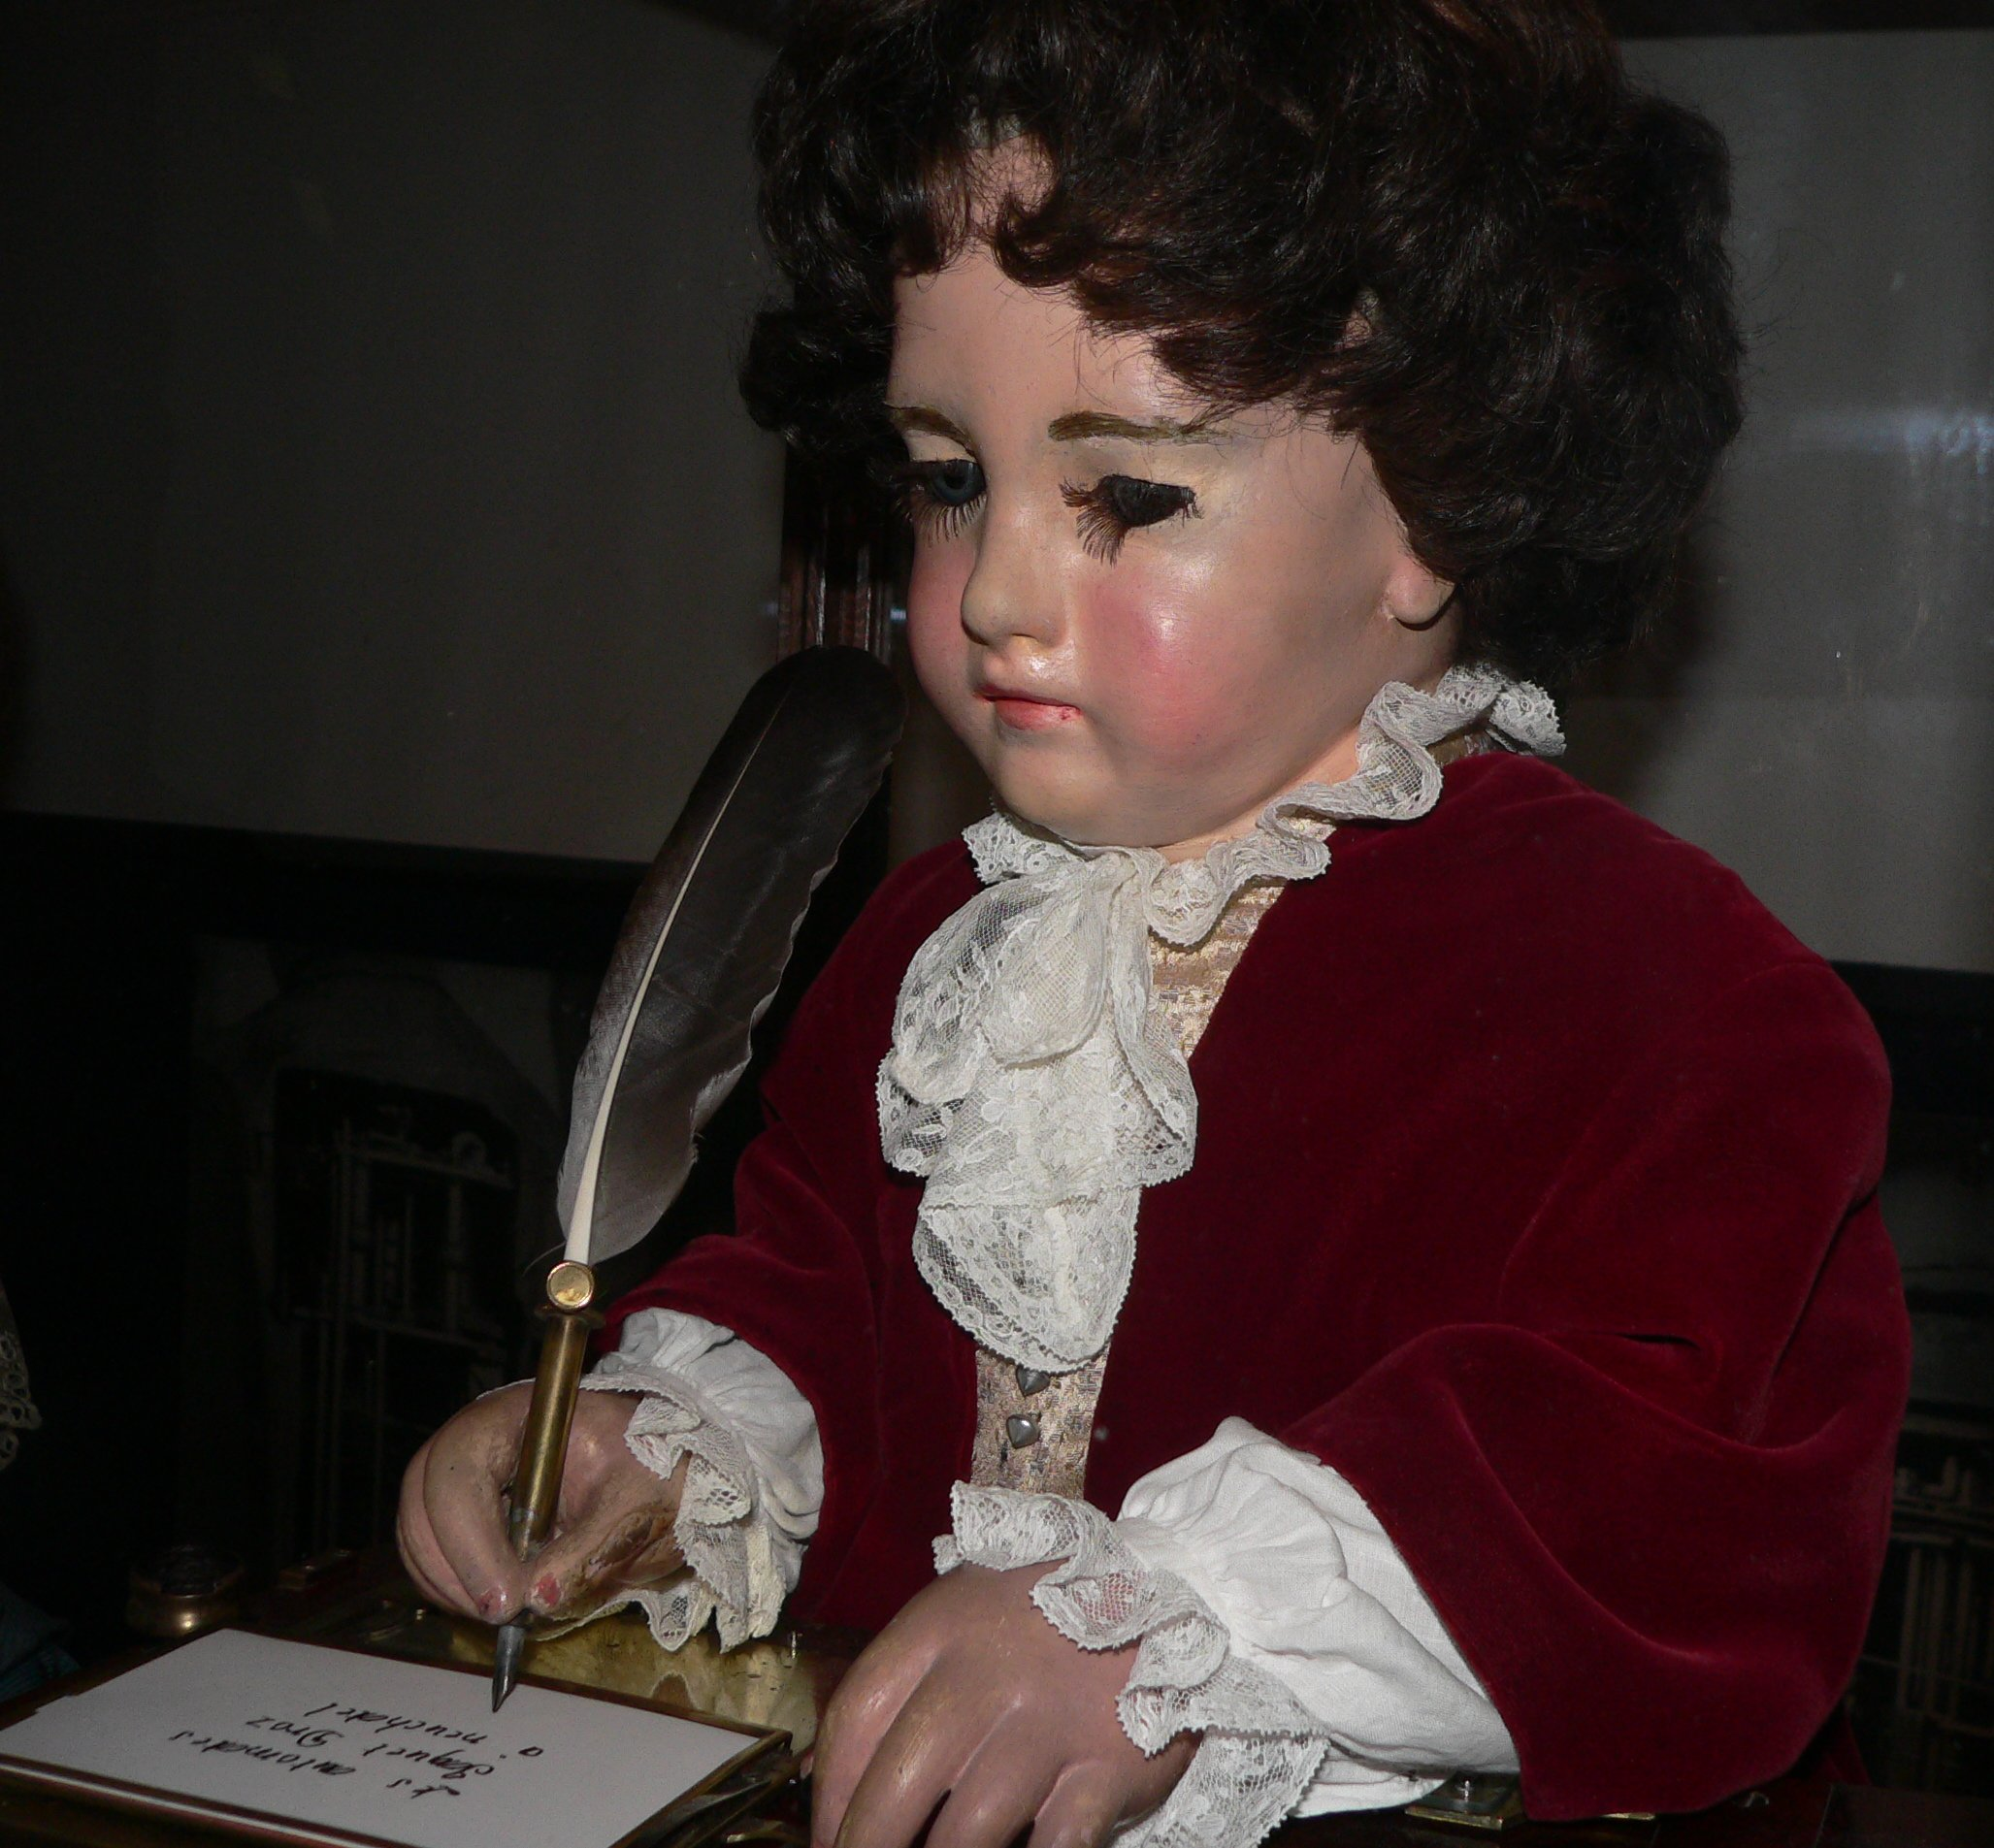
\includegraphics[width=5cm]{automate_jaquet_droz.jpg}
					\caption{Les automates Jaquet-Droz, l'Ecrivain, musée d'Art et d'Histoire de Neuchâtel, source Wikimedia Commons, auteur Rama}
					\label{fig:automate_jaquet_droz}
				\end{figure}
				Nous verrons que l'exemple suivant -- celui du robot Calliope -- présente la tendance inverse~: peu d'importance accordée à la mécanique et à l'aspect anthropomorphe, mais en revanche une grande attention portée au programme de génération de texte.
			\subsubsection{Le robot Calliope d'Albert Ducrocq et Louis Couffignal}\label{calliope}
				Le ``projet Calliope'' est bien plus qu'un simple algorithme, puisque Calliope est une machine communicante. Prénommée d'après la Muse de la poésie épique et de l'éloquence par ses créateurs Albert Ducrocq (cybernéticien, journaliste et essayiste) et Louis Couffignal (mathématicien et cybernéticien), Calliope était capable de ``créer'' des poèmes et de les transmettre au spectateur/auditeur. Nous nous appuierons dans cette partie sur les commentaires de Philippe Bootz dans \cite{bootz}.\\
				\subsubsubsection{Mode de fonctionnement de Calliope}
					Du côté de l'algorithme, Calliope génère des énoncés relativement primaires, sous la forme d'un triplet sujet-prédicat-objet. Le modèle, selon Philippe Bootz, est proche des premiers modèles utilisés par Jean-Pierre Balpe (dont nous parlerons plus amplement en Section \ref{balpe}) dans les années 80.\\
					Du côté matériel, Calliope est une sorte de boîte qui transmet ses messages à l'aide de \textit{flashes} lumineux binaires (rouges pour $1$ ou verts pour $0$). Un poème de Calliope est donc, en pratique, une chaîne de bits. Le prédicat est séparé du sujet par une chaîne de 2 ou 3 bits initialisés à 0 (soit 2 ou 3 flashs verts selon le contexte). Chaque mot est une séquence de bits de longueur arbitraire, dont la taille varie avec le degré de précision du mot. En effet, les mots du lexique de Calliope sont alignés sur un arbre binaire, et sont par conséquents organisés selon une taxonomie sémique~:\footnote{il est intéressant de voir que ce genre d'organisation est toujours d'actualités dans nos lexiques actuels ! L'exemple le plus connu pour la langue française est sans doute le projet WOLF (Wordnet libre du français), qui regroupe un très grand nombre de léxèmes du français selon une arborescence (non binaire), chaque sous arbre étant appelé \textit{synset} (pour ``ensemble de synonymes'').}.
					\vspace{2mm}
					\begin{itemize}
						\item Les sujets et les objets (les ``êtres'') sont des substantifs, mais leur sémantique inclut dans certain cas la sémantique de modifieurs potentiels (adjectifs, qualificatifs, articles);
						\item Les prédicats (ou ``instructions'') sont des verbes où des adverbes.
					\end{itemize} 
					\vspace{2mm}
					Compte tenu de la diversité des mots possibles et des contraintes de désambiguïsation\footnote{chaque mot commence par un radical de 4 bits, les êtres commencent par un 1 et les instructions par un 0...}, la longueur moyenne d'un phrase de Calliope est située autour de 65 bits. Le processus de décodage est donc relativement fastidieux, et fait partie intégrante de l'expérience. Les erreurs de lecture sont probables~: comme le précise Philippe Bootz, le choix du moment de l'arrêt de la machine influence le \textit{parsing} (segmentation) du code binaire, et peut donc modifier les mots décodés. De plus, la sémantique du message décodé -- un message souvent très sommaire, très sibyllin -- demeure à l'appréciation de l'expérimentateur. C'est donc bien lui qui élabore encore en grande partie le contenu poétique du message de Calliope.
					\begin{citationbox}
						\textit{Autrement dit, contrairement à
						un texte généré, la qualité textuelle, au regard de règles d'appréciation d'un texte
						imprimé du genre poème surréaliste, dépend plus du ``traducteur'' que de
						Calliope. On est finalement assez loin du robot poète}
					\begin{flushright}
						Philippe Bootz, \textit{Un historique de la génération numérique de textes} \cite{bootz}
					\end{flushright}
					\end{citationbox}
				\subsubsubsection{``Polémiques'' autour de Calliope}
					Le robot Calliope a provoqué des remous en France, où l'on s'inquiétait de voir la machine supplanter l'humain. Cela a sans doute été accentué par le fait que Calliope, contrairement aux \textit{Love Letters} ou aux \textit{Textes Stochastiques} produits à la même époque, était quelque chose d'``incarné'', de tangible. En particulier, Philippe Bootz dans \cite{bootz} rapporte qu'André Parinaud, rédacteur de la revue \textit{Arts} s'inquiétait du ``robot-poète'' d'Albert Ducrocq. Cette inquiétude s'est soldée par une réponse caustique de Boris Vian, qui dans une longue lettre à André Parinaud en a profité pour plaisanter sur Victor Hugo en ces termes~:
					\begin{citationbox}
						\textit{Voilà, mon Parinaud, les dangers de la demi-culture; car il il vous suffit de voir en un journal du matin que monsieur Albert Ducrocq a construit un robot-poète pour vous étonner aussitôt. Pourtant, qu'est-ce que ça a d'extraordinaire puisqu'on connaît Victor Hugo depuis longtemps~? [...] Il y a maintenant des tas d'appareils qui choisissent divers trucs parmi divers autres trucs possibles et manifestent de la sorte une espèce de caractère.}
						\begin{flushright}
							Boris Vian, \textit{``Un robot-poète ne nous fait pas peur'', Lettre à André Parinaud}, avril 1953  \cite{vian1953}
						\end{flushright}
					\end{citationbox}
					
					La seconde ``polémique''\footnote{le terme est peut-être un peu fort pour cet exemple...} liée à Calliope a été provoquée par une expérience de Louis Couffignal, qui s'était chargé modifier la Calliope originelle pour en faire un programme capable d'écrire de véritables poèmes à l'aide d'un lexique littéraire de $300$ mots et de règles de grammaire adaptées\footnote{la composante robotique de Calliope a donc été abandonnée dans le cadre de ce test}. Le test de Couffignal, mentionné par Philippe Bootz, ressemble à un test de Turing (cf. Section \ref{test_turing}). Il s'agissait de présenter à un jury des vers de Calliope et des vers de Paul Eluard, et de poser deux questions~:
					\vspace{2mm}
					\begin{itemize}
						\item quels sont les vers les plus poétiques ?
						\item  quels sont les vers les plus robotiques ?
					\end{itemize}
					\vspace{2mm}
					Le test a notamment été mené en 1965 lors des rencontres internationales de Genève. Les vers de Calliope présentés à cette occasion, qui commençaient par ``\textit{Un doute agréable couleur de lotus endormi [...]''}, sont restés assez célèbres. Cela dit, ces vers ont été choisis pour leur style, leur ``littérarité'' par Louis Couffignal lui-même, parmi près de $150$ productions. On peut donc penser qu'ils n'étaient pas très représentatifs des capacités réelles de Calliope, qui devaient être en moyenne plus basses. De plus, comme on l'a dit plus haut, le vocabulaire de Calliope, restreint mais sélectionné sur le volet, favorisait grandement la production de syntagmes ``poétiques''. L'auteur, s'il n'agissait pas en sortie du système comme dans le cas de la ``première'' Calliope, imposait tout de même sa marque d'une façon non négligeable \textit{en entrée} cette fois-ci.\\
					
					Lors des rencontres de Genève, Calliope et Eluard sont arrivés à peu près \textit{ex aequo} en ce qui concerne le caractère poétique; et environ 6 personnes sur 10 ont réussi à ``démasquer'' Calliope. On peut donc en déduire qu'un sous ensemble non négligeable du jury à considéré les vers de Calliope comme plus poétiques en \textit{sachant} qu'ils s'agissait des vers d'un robot.\\
					
					La robotique et la génération de texte semblaient donc être dans les années cinquante des domaines clivants, avec leur adeptes, leurs détracteurs, mais aussi beaucoup de simples observateurs, curieux des évolutions futures de tels systèmes.
			\subsubsection{L'ORLANoïde}
				L'ORLANoïde est un androïde -- ou plutôt une gynoïde -- que nous avons eu l'occasion de ``rencontrer'' durant l'exposition \textit{Artistes et Robots} au Grand Palais \cite{artistes_robots}, exposition pour laquelle l'ORLANoïde avait été spécialement conçue. Comme Calliope, l'ORLANoïde est une œuvre collaborative, qui a réuni une plasticienne, ORLAN, et un poète-programmeur, Jean-Pierre Balpe (l'ensemble de la section suivante lui sera aussi consacré). Cette œuvre, en plus d'interroger le statut du langage, aborde le thème du corps et du double.\\
				
				En effet, l'ORLANoïde, comme son nom l'indique, est un robot fait à l'image de son auteure, du moins pour le buste, couvert de silicone et reproduisant ainsi le visage, les traits et les accessoires d'ORLAN. Le reste du corps est laissé dans son état purement ``fonctionnel'', avec la mécanique apparente, sauf pour le cœur, visible par effet de transparence. L'image du robot se dédouble à l'infini grâce à un jeu de miroirs. Le but pour ORLAN était ainsi de faire de son propre corps ``le lieu du débat public''.\\
				Car une autre caractéristique de l'ORLANoïde est qu'elle dialogue directement avec sa créatrice \textit{via} deux télévisions \footnote{et indirectement avec le public, suivant un principe que l'on pourrait qualifier de \textit{double énonciation théâtrale}...}. Le dédoublement est donc total. Et ce dédoublement conduit évidemment à se demander qui est qui, et à qui attribuer les dialogues...
				\begin{citationbox}
					\textit{Poursuivant sa démarche artistique sur le corps, l’artiste ORLAN a créé un robot à son image, l’ORLANOÏDE avec lequel elle compte dialoguer en public. Pour cela, elle m’a demandé de créer un générateur de questions que cet avatar pourrait lui poser. Parfois, l’ORLANOÏDE cite ORLAN, bien sûr en majuscules.}\begin{flushright}
						Jean-Pierre Balpe, \textit{Site officiel} \cite{balpe_site}
					\end{flushright}
				\end{citationbox}
				... d'autant plus que ces dialogues sont générés à l'aide d'un algorithme crée par Jean-Pierre Balpe. Selon la communication officielle de l'exposition, le générateur s'appuie sur le \textit{deep learning}, une forme d'apprentissage statistique récente et très performante (comme nous le verrons en Section \ref{neural_net}). Cet algorithme producteur des questions posées par l'ORLANoïde à sa créatrice est librement testable sur la page \href{http://www.balpe.name/Questions-de-l-Orlanoide-a-ORLAN}{http://www.balpe.name/Questions-de-l-Orlanoide-a-ORLAN}. Nous recopions ci-dessous deux des \textit{outputs} que nous avons obtenus~:
				\begin{citationbox}
					\textit{Je n'ai pas réellement besoin de ça, de cet ORLANOÏDE. UN TEXTE D’ENGAGEMENT. Qu'est-ce que cela fait d’avoir son double en face de toi ? Avons-nous le même cœur ? L'ORLANOÏDE est distant ? Tu es une mutante, les transformations que tu as opérées sur ton corps ont-elles des conséquences sur ton esprit. CATHÉDRALE DE VERRE. L'océan n'est-il pas à regarder ? RECONSTITUTION.}
					\begin{flushright}
						Jean-Pierre Balpe, \textit{Questions de l'ORLANoïde à ORLAN} \cite{balpe_site}
					\end{flushright}
				\end{citationbox}
				\begin{citationbox}
					\textit{NE SUIS-JE QU'UNE FICTION. Aristote a dit : il n'y a pas de génie sans un grain de folie ; qu’en penses-tu. Tel est le temps pour moi. Avec tous ces hybrides, l’Europe culturelle c'est foutu ? Que peut être cette ORLANOÏDE. N'importe quoi n'est pas perpétuellement n'importe quoi ? M'unir à ORLAN par la moule par les paroles du con ? Dire ce que je suis et ce que je ne suis pas ?}
					\begin{flushright}
						Jean-Pierre Balpe, \textit{Questions de l'ORLANoïde à ORLAN} \cite{balpe_site}
					\end{flushright}
				\end{citationbox}
				Nous voyons que l'ORLANoïde s'exprime relativement clairement, avec des phrases syntaxiquement correctes; même si le lien sémantique entre les différentes phrases est parfois obscur \footnote{et pour cause, les modèles statistiques ne connaissent pas de règles sémantiques \textit{a priori}}. Elle semble posséder un genre de culture générale superficielle, ce qui lui permet de citer Aristote et de mentionner l'Europe. Ce genre de phénomène ne peut survenir que lorsque le modèle d'apprentissage est suffisamment complexe (en règle générale, plus le modèle est complexe et ``profond'', plus le degré d'abstraction peut être fort) et le corpus suffisamment riche. Tout cela rapproche l'ORLANoïde de Benjamin, une IA créatrice d'un script de court-métrage dont nous parlerons en Section \ref{fiction_vs_realite}. En effet, ces deux programmes remettent réellement en cause l'unité de l'auteur. Dans le cas de l'ORLANoïde, cette diffraction s'opère aussi bien théoriquement (problème de l'attribution) que techniquement (dédoublement physique au travers du robot).
				
		\subsection{Jean-Pierre Balpe~: ``poète de synthèse''}\label{balpe}
			Jean-Pierre Balpe est un écrivain et chercheur dans le domaine de la relation entre littérature et informatique. Il a notamment été directeur du département Hypermédia de l'Université Paris VIII entre 1990 et 2005, et Secrétaire Général de la revue \textit{Action Poétique} entre 1974 et 2010 \cite{wiki:jp_balpe}. Pendant un temps membres de l'ALAMO, il a aussi activement contribué à la revue informatique \textit{KAOS}. Selon Philippe Bootz~:
			\begin{citationbox}
				\textit{Jean-Pierre Balpe is a unique personality in the field of French digital literature. He played an important role in the evolution of this literature, on one hand by his conceptions that could not remain indifferent, and on the other hand by the position he has held in various organizations.}
				\begin{flushright}
					Philippe Bootz, \textit{From OULIPO to Transitoire Observable} \cite{bootz2012}
				\end{flushright}
			\end{citationbox}
			Nous consacrons donc une section entière à Jean-Pierre Balpe, car ses productions littéraires sont extrêmement diverses et mettent notre approche typologie à l'épreuve. Jean-Pierre Balpe à écrit des livres bien sûr, mais aussi des poèmes, des nouvelles et des essais publiés dans des revues (\textit{Action poétique} évidemment, \textit{Autrement}, \textit{Æncrages \& Co}, \textit{Europe}...).\\
			
			Mais c'est surtout par rapport aux supports ``modernes'' que Jean-Pierre Balpe se distingue. Car contrairement à ses prédécesseurs Christopher Strachey et Theo Lutz, Jean-Pierre Balpe exploite à fond le médium informatique~: plus question donc d'imprimer les textes, tout se passe à l'écran, et même, sur \textit{les} écrans, car les productions de Jean-Pierre Balpe sont nombreuses à être directement accessibles sur Internet (sur son site personnel \href{http://www.balpe.name/}{http://www.balpe.name/} ou même Facebook).
			\begin{citationbox}
				\textit{Dire qu’un dispositif informatique est utilisé comme médium signifie en tout premier lieu que l’ordinateur est utilisé par l’auteur pour créer l’œuvre littéraire et par le lecteur pour la lire. Autrement dit, l’œuvre littéraire ne quitte jamais totalement le dispositif informatique. C’est en cela qu’il en constitue le médium.}
				\begin{flushright}
					Philippe Bootz, \textit{Les Basiques~: la littérature numérique} \cite{bootz2006}
				\end{flushright}
			\end{citationbox}
			Auteur ``syncrétique'' Balpe emprunte tour à tour quasiment toutes les voies ouvertes par la littérature générative~: la génération ``classique'' par algorithme (\textit{Poèmes Stein}\cite{balpe_stein}, \textit{Proust Memories} \cite{balpe_proust}, l'hypertexte de fiction \cite{balpe_disparition}, la littérature générative multimédia \cite{balpe_videoseries}. De plus, ses techniques de génération, plus poussées que celles de ses prédécesseurs, prennent en compte l'ensemble des niveaux linguistiques, du lexique à la sémantique, en passant par la syntaxe.
			\begin{citationbox}
				\textit{Jean-Pierre Balpe has since 1975 developed a concept of generation different from that prevailing in the OULIPO. It takes into account the semantic and pragmatic levels of the generation process. His work is based on researches in natural languages processing at the contrary of combinatory generation.}
				\begin{flushright}
					Philippe Bootz, \textit{From OULIPO to Transitoire Observable} \cite{bootz2012}
				\end{flushright}
			\end{citationbox}
			
			\subsubsection{\textit{La Disparition du Général Proust}}
				\subsubsubsection{Une œuvre hypertextuelle...}
					\begin{citationbox}
						\textit{L'hyperfiction \textit{La Disparition du Général Proust} est une réflexion en acte, donc en textes, sur ce que le numérique peut apporter à l'écriture littéraire.}
						\begin{flushright}
							Jean-Pierre Balpe, \textit{Comment La Disparition du Général Proust} \cite{balpe_blog}
						\end{flushright}
					\end{citationbox}
					Travail sur le contenu est sur son médium, cette œuvre tentaculaire (à défaut d'être une ``œuvre cathédrale''(!)) rassemble différents textes générés par ordinateur et offrant un ``thème et variations'' autour de l'œuvre de Marcel Proust. L'idée est venue à Jean-Pierre Balpe de façon progressive ; aussi le projet s'est-il étendu sur plusieurs décennies :
					\begin{citationbox}
						\textit{Le travail concret, réel, sur \textit{La Disparition du Général Proust}, a commencé vers 1980 (je ne saurais donner une date plus précise) et s'est appuyé sur mes travaux antérieurs. Près de 40 ans donc de recherche sur la génération automatique de textes littéraires.}
						\begin{flushright}
							Jean-Pierre Balpe, \textit{Mon site personnel} \cite{balpe_blog}
						\end{flushright}
					\end{citationbox}
					\textit{La Disparition du Général Proust} consistait donc au départ en un ensemble de textes générés  dans  des langages de programmation comme APL, Basic, ou Hypercard. Les technologies et les standards ayant rapidement évolué, un grand nombre des travaux originaux liée à ce projet ont été ``perdus'',  quoique toujours présents sur des disquettes désormais illisibles.\\
					
					Pour autant, Jean-Pierre Balpe dit avoir restauré avec l'aide de Samuel Szoniecky et de l'entreprise Digitalarti bon nombre des générateurs de textes originaux. Ces générateurs furent d'abord mis en place (à partir de 2006) sur un ``réseau'' de blogs connectés entre eux par des liens hypertextes. Ces blogs étaient au nombre de 19, et accompagnés de 5 albums photo \cite{bordeleau2009}. A l'heure actuelle, ces sites ne sont malheureusement plus maintenus, mais ont été remplacés par un ``point d'entrée'' sur le site principal de Jean-Pierre Balpe. La fiction a donc migré des sites variés vers un unique site web, au sein de différentes pages appelées ``Dédales''.
					\begin{citationbox}
						\textit{Cette nouvelle présentation m'a ainsi amené à reconsidérer La Disparition du Général Proust (cf. aussi plusieurs articles dans ce blog) en définissant un nouveau mode de circulation dans cette vaste hyperfiction sans porter atteinte à celui établi par un ensemble de blogs reliés. Cette œuvre devient ainsi encore plus réticulaire et impossible à définir dans les termes d'une définition non numérique de la littérature.}\begin{flushright}
							Jean-Pierre Balpe, \textit{Mon site personnel}\cite{balpe_blog}
						\end{flushright}
					\end{citationbox}
					Il en effet difficile de savoir qu'est-ce qui, dans la totalité de l'œuvre de Jean-Pierre Balpe, fait ou ne fait pas partie de \textit{La Disparition du Général Proust}, tant les pages sont nombreuses et les miroirs nombreux (par exemple, le site \href{http://sensdelavie.canalblog.com/}{http://sensdelavie.canalblog.com/} qui semble encore être maintenu...). \textit{La Disparition du Général Proust} est une nébuleuse informatique, d'un type qu'ils serait difficile de concevoir hors du média numérique (où la notion de publication, de série, d'édition sont beaucoup plus tranchées~!).\\
					
					Quoi qu'il en soit -- hypertextes inter-site ou intra-site -- le trait le plus saillant de cette œuvre numérique est sans doute son organisation non linéaire voire circulaire, jouant des indirections (et même peut être des liens morts, des doublons~!), à mettre en perspective avec ces paroles de Jacques-Athanase Gilbert~:
					\begin{citationbox}
						\textit{Il est intéressant de mettre en rapport l’obsolescence programmée des technologies avec la volonté de tout conserver et enregistrer. Nous vivons dans une sorte de présentisme anhistorique alors même que nous vivons paradoxalement une époque de patrimonialisation intense.}
						\begin{flushright}
							Jacques-Athanase Gilbert, \textit{Entretien ``Carnet de recherche'' (OBVIL)} \cite{gilbert2018}
						\end{flushright}
					\end{citationbox}
				\subsubsubsection{...qui met à mal la notion d'auteur}
					Une autre caractéristique de \textit{La Disparition du Général Proust} est l'abolition des différences entre le réel et le virtuel, l'humain et le non-humain. Jean-Pierre Balpe cultive en effet dans ses blogs trois types d'identités~:
					\vspace{2mm}
					\begin{itemize}
						\item des avatars derrière lesquelles se cache Jean-Pierre Balpe : Marc Hodges (la \textit{némésis} de l'auteur~!), Nathalie Riches...
						\item des personnalités entièrement fictives dont les ``écrits'' sont générés par ordinateur : Pierre Charlus, Germaine Proust...
						\item Jean-Pierre Balpe lui-même, quand il signe sous son vrai nom (notamment sur son site personnel, \href{http://poetiques.blogg.org/}{http://poetiques.blogg.org/})
					\end{itemize}
					\vspace{2mm}
					Un récapitulatif de ces différents types d'identités narratives est compilé dans le Tableau \ref{tab:balpe_identites}.
					\begin{table}
						\centering
						\begin{tabular}{c | c c}
							&``Vraie'' personne & Personne fictive \\ \hline
							``Vrai'' discours & J.-P. Balpe & Marc Hodges, Nathalie Riches...\\
							Discours généré &~?? & Germaine Proust, Pierre Charlus...
						\end{tabular}
						\caption{Un tableau récapitulatif des jeux d'identités de Jean-Pierre Balpe dans \textit{La Disparition du Général Proust}}
						\label{tab:balpe_identites}
					\end{table}
					Ce perpétuel dédoublement met dès lors le lecteur dans le doute : dans quelle mesure le texte qu'il est en train de lire est-il ``réel'', autrement dit, écrit pas un humain ? De ce doute surgit également un questionnement : l'hésitation ``naturelle'' vis-à-vis de l'origine d'un texte est-elle vraiment légitime ? Ne faudrait-il pas revoir nos propres standards en matière de littérature, et accepter un texte tel qu'il est, sans considération pour les modalités de sa production ou pour son auteur ? Nous reviendrons plus amplement sur ces questions cruciales à la Section \ref{nouvelle_definition}.\\
					
					En attendant, nous nous intéresserons  dans la section suivante à deux générateurs de texte faisant partie de l'hyperfiction \textit{La Disparition du Général Proust}.
			
			\subsubsection{Deux générateurs de texte~: \textit{Proust Memories} et \textit{Poèmes Stein}}
				\begin{citationbox}
					\textit{Les générateurs automatiques développés par Jean-Pierre Balpe depuis les années 80
					se distinguent des générateurs combinatoires oulipiens. Ils utilisent des algorithmes qui ne
					combinent pas des paradigmes dans des syntagmes mais qui construisent des textes à partir
					d’un dictionnaire et d’une grammaire qui se développe sur une approche pragmatique du
					domaine sémantique exploré par le texte. Il est même possible de recréer le style d’un auteur. }
					\begin{flushright}
						Philippe Bootz, \textit{Poésie numérique : la littérature dépasse-t-elle le
						texte ?}\cite{bootz2005}
					\end{flushright}
				\end{citationbox}
				Les deux générateurs de textes \textit{Proust Memories} (\href{http://proustmemories.canalblog.com/}{http://proustmemories.canalblog.com/}) et \textit{Poèmes Stein} parviennent effectivement à reproduire le ``style'' du romancier français et de la poétesse américaine (\href{http://brooom.org/balpe/photoCadre.html}{http://brooom.org/balpe/photoCadre.html}).\\ 
				
				En revanche, les modes de fonctionnement de ces deux générateurs de texte semblent relativement différents. D'un côté, \textit{Proust Memories} semble opérer par \textit{patchworks} de textes issus de \textit{La Recherche}, moyennant l'ajout de quelques mots de liaison. D'un autre côté, \textit{Poèmes Stein} semble produire ses échantillons \textit{ex nihilo}, en partant d'un simple lexique de mots (d'où une correction syntaxique plus faible que dans \textit{Proust memories} -- mais somme toute cela coïncide bien avec le style Gertrude Stein comme on pourra le constater Section \ref{inversion_paradigme}). 
				
				\begin{citationbox}
				\textit{Que ce soit Proust Memories dont le texte est un centon infini ajusté par un algorithme relativement simple jusqu'aux Poèmes Stein (sous leurs diverses formes et, bien entendu, avec quelques traitemenst Steiniens) [...]}
					\begin{flushright}
						Jean-Pierre Balpe, \textit{Mon site personnel} \cite{balpe_blog}
					\end{flushright}
				\end{citationbox}
				
				En outre, les deux générateurs diffèrent dans leurs modes de présentation. Dans \textit{Proust Memories}, des ``Rêves'' préalablement générés se succèdent et prennent la forme de billets de blog. Nous sommes donc face à une présentation linéaire, relativement traditionnelle puisqu'elle se rapproche de par sa verticalité des sites web habituels mais aussi du \textit{volumen} antique. Cette présentation brouille donc davantage les pistes quant à la nature du discours (``réel'' ou généré ?).\\
				Les \textit{Poèmes Stein} exploitent beaucoup plus les potentialités du médium informatique; en effet, les poèmes sont générés \textit{on the fly} et portés à l'écran, ils sont aussi accompagnés d'une image de fond qui change à chaque rafraîchissement de la page. Nous sommes donc dans un principe plus moderne de non-linéarité, dans une logique du ``recouvrement'', du palimpseste. A cet égard, Philippe Bootz, reprenant l'expression de Jean Clément, parle d'\textit{esthétique de la frustration}~:
				\begin{citationbox}
					\textit{Le terme ``esthétique de la frustration'' a été forgé en 1993 [...] C’est Jean Clément qui avait
					relevé le caractère frustrant de cette poésie qu’on ne peut relire [...] L’esthétique de
					la frustration consiste à attribuer, dans le projet d’écriture, une valeur sémiotique à l’activité et
					aux réactions du lecteur. Autrement dit, à considérer que l’activité de lecture elle-même, dans
					son aspect béhavioriste, fait partie du texte.}
					\begin{flushright}
						Philippe Bootz, \textit{Poésie numérique : la littérature dépasse-t-elle le texte ?} \cite{bootz2005}
					\end{flushright} 
				\end{citationbox}
				
				
				Quoique plus en accord avec le support internet, multimédia et interactif, la présentation des \textit{Poèmes Stein} est certainement moins équivoque que celle de \textit{Proust Memories}, dans la mesure où la génération du texte ``se fait sentir'' au moment du clic déclencheur (on imagine facilement le clic appeler un script...).\\
				
				Mais il demeure que dans ces deux cas, la question de l'attribution se pose très clairement : comment dire qu'une œuvre littéraire est sans équivoque ``typique de Proust'' ou ``typique de Stein'', quand un algorithme est susceptible de produire des exemples aussi convaincants ? A ce sujet, Jean-Pierre Balpe irait jusqu'à dire que les algorithmes de génération de texte sont -- en puissance -- supérieurs à l'écrivain humain...
				\begin{citationbox}
					\textit{Ce qui m’intéresse dans la génération, ce n’est pas le texte qui s’affiche. Ce texte-là est
				un moment comme un autre, on s’en fout. [...] Ce qui m’intéresse, c’est cette capacité à
				produire à l’infini et à générer un univers que je ne suis pas capable de faire. C’est donc un
				autre substitut qui transmet une pensée qui dit. Peut-être est-ce un fantasme d’éternité.}
					\begin{flushright}
						Jean-Pierre Balpe, \textit{A:{$\backslash$ LITTERATURE $\hookleftarrow$}}\cite{balpebootz1994}
					\end{flushright}
				\end{citationbox}

				
			\subsubsection{Une projet sériel, génératif et multimédia~: les \textit{Vidéoséries}}
				\begin{citationbox}
					\textit{Nous nommerons ``transitoire observable'' la partie de l’œuvre produite par le programme et accessible à la lecture. Le transitoire observable est l’événement multimédia produit par l'exécution du programme et proposé à la lecture.}
					\begin{flushright}
						Philippe Bootz, \textit{Les Basiques~: la littérature numérique} \cite{bootz2006}
					\end{flushright}
				\end{citationbox}
				Nous nous penchons ici sur un projet plus récent de Jean-Pierre Balpe, plus ``syncrétique'' également. Il s'agit du projet des ``vidéoséries'' publiées sous le format standard saison-épisode sur la page \href{http://www.balpe.name/-Dedale-des-Videoseries-}{http://www.balpe.name/-Dedale-des-Videoseries-}. Ces vidéoséries semblent en effet répondre à un manque de la littérature ``informatisée'' que Jean-Pierre exprimait en 1994 dans \textit{Un roman inachevé -- Dispositifs} : 
				\begin{citationbox}
					\textit{L'aspect visuel du texte, largement contraint par les conventions du médium employé, souffre de ne pouvoir exploiter tous les possibles de l'image, puis ceux de l'image en mouvement.}
					\begin{flushright}
						Jean-Pierre Balpe, \textit{Un roman inachevé -- Dispositifs} \cite{balpe1994}
					\end{flushright}
				\end{citationbox}
				Voici comment l'auteur lui même présente le projet~:
				\begin{citationbox}
					\textit{Le Dédale des Vidéoséries propose un ensemble de courtes vidéos qui, toujours sur la base de la génération automatique de textes, se proposent de travailler sur les rhétoriques du genre : pauvreté des situations, simplification psychologique, répétitions, variations... Mais ceci en utilisant les outils gratuits disponibles dans l'espace Internet et en s'appuyant sur des créations volontairement pauvres.}
					\begin{flushright}
						Jean-Pierre Balpe, \textit{Site officiel} \cite{balpe_site}
					\end{flushright}
				\end{citationbox}
				
				Ces  \textit{Vidéoséries} sont publiées depuis avril 2018 dans des billets de blog, par des identités diverses : Pierre Charlus, Paul Méphisto, Germaine Proust, Sylvester Saint-Loup (!)... compte tenu de ce qui a déjà été dit jusque là sur les travaux de Jean-Pierre Balpe, il n'est pas surprenant que ces identités soient fictives.    Chaque identité est associée à un ``photo de profil'' ou plutôt un portrait peint. Les vidéos en elles-mêmes ont un format court ($2$ minutes $30$ en moyenne), et allient contenu texte, film et voix-off.\\
				
				Les films de fond sont globalement très contemplatifs : pas de situation de dialogue entre interlocuteurs, et souvent pas d'individu dans le champ de la caméra. Le contenu texte qui vient se calquer au dessus du film est parfois compréhensible, mais souvent totalement flou (lettres entrelacées, qui se chevauchent de façon anarchique...). Faisant écho au texte à l'écran, les voix-off débitent des vers ou des fragments de récits générés par ordinateur sur une voix monocorde, elle aussi générée synthétiquement.\\
				
				Jean-Pierre Balpe intègre dans ce projet récent texte, typographie, animation, vidéo, musique et parole dans un tout cohérent. L'ensemble des médias convoqués vont dans un même sens~: développer une véritable identité du texte généré, lui donner corps. Jean-Pierre Balpe utilise bien ici la rhétorique du ``Transitoire Observable'' introduite par Philippe Bootz. Le projet des Vidéoséries reprend aussi très bien ces propos d'Ambroise Barras~:
				\begin{citationbox}
					\textit{un ``texte à
						l'ordinateur'' n'est pas le substitut, vague et désolant ersatz, d'un ``texte en
						livre''.}
					\begin{flushright}
						Ambroise Barras, \textit{Prolégomènes à toute littérature informatique} \cite{barras1995}
					\end{flushright}
				\end{citationbox}
				
				
				Nous pensons avoir retracé dans cette Section un panorama historique des générateurs de texte. Bien sûr, le domaine est bien plus vaste que ce qui a été exposé ici, et on aurait pu davantage aborder la création hypertextuelle et la création multimédia. Mais nous avons décidé de nous focaliser sur les \textit{méthodes} de génération pour mieux faire le lien avec la section qui va suivre, plus technique, plus proche de l'informatique et de l'ingénierie.
%				\begin{citationbox}
%					\textit{S'intéresser aux rapports entre littérature et informatique, ce sera dès lors rendre compte des implications complexes entre texte, machine et programme. Comme nous pouvons déjà le suspecter, il ne sera plus possible de parler de texte de façon autonome~: il n'y aura plus de texte. Il y aura en revanche un système ``texte-programme-machine'', une configuration complexe dont les frontières resteront floues et intriquées.}
%					\begin{flushright}
%						Ambroise Barras, \textit{Prolégomènes à toute littérature informatique} \cite{barras1995}
%					\end{flushright}
%				\end{citationbox}
				
				
				
				
				
				
				
				
				
				
				
				
			
				
				

				
				
	
% Philippe Bootz et Camille Paloques-Bergès, ou les américains Charles Hartman et Christopher Funkhouser guilet
% nouvelles formes d'expérimentation littéraire comme 5l'animation de texte (1982) et l'hypertexte de fiction (1987) guilet

%hypertexte Jardin aux sentiers qui bifurquent borges bonnet
		\newpage
	\section{Aspects techniques de la littérature générative}\label{aspects_tech}
		De nos jours, la génération de texte s'est élargie et touche beaucoup plus de domaines qu'à ses débuts. De nature purement artistique et expérimentale pour nos poètes programmeurs et autres groupes littéraires d'avant-garde, la génération de texte sert actuellement à créer des résumés synthétiques pour les grandes entreprises \footnote{Yseop par exemple, propose aux entreprises des secteurs de la finance, de la \textit{business intelligence} et du marketing des solutions pour la génération de rapports et de résumés à partir de données de tableur.}, à interagir en temps réel avec des utilisateurs ou des consommateurs (\textit{chatbots}) à générer le nom de sa nouvelle marque en fonction des caractéristiques que l'on souhaite  mettre en avant \footnote{un service proposé gratuitement par Namelix sur la page \href{https://namelix.com/}{https://namelix.com/}, en plus de générer une typographie} ou même à produire des bulletins météo \footnote{le système le plus ancien à avoir été déployé est le système FoG. Ce système a été utilisé par le Canada pour générer des bulletins météo en français et en anglais au début des années 90 \cite{wiki:fog}.}.\\
		
		Les raisons de cette expansion sont d'ordre économique et technique~: c'est avec l'amélioration de la puissance de calcul et des algorithmes que ce sont ouverts de nouveaux créneaux commerciaux pour ce que l'on appelle désormais le Natural Language Processing (NLP) ou Natural Language Generation (NLG). Et en retour ces enjeux économiques ont eu tendance à supporter (mais aussi orienter) la recherche.\\
		\begin{citationbox}
			\textit{D’abord, l’apparition d’une masse de données monstrueuse, liée au développement d’Internet. Les algorithmes ont besoin de beaucoup de données pour s’améliorer continuellement. Ensuite, l’augmentation de la puissance de calcul liée à la loi de Moore, qui a permis de faire tourner ces mêmes algos, qui étaient bloqués dix ans auparavant. Enfin, les investissements de Google et Facebook et, dans une moindre mesure, des Canadiens avec leur programme CIFAR [...]}
			\begin{flushright}
				Gilles Moyse, \textit{Entretien pour la revue Usbek et Rica} \cite{edin2018}
			\end{flushright}
		\end{citationbox}
		Nous sommes d'avis que repenser la littérarité en fonction des apports de l'ordinateur nécessite de se plonger dans les aspects techniques des algorithmes utilisés, pour mieux cerner les mécanismes en action, le rôle du programmeur, mais aussi les caractéristiques de l'\textit{output}. Dans cette partie nous tenterons donc d'établir une typologie des méthodes employées en NLG et de mettre ces méthodes en perspective par rapport au problème de la littérature. Cette approche typologique nous permettra également de préciser certaines notions introduites en dans la section \ref{genealogie}. Nous proposons une typologie en deux temps~: d'abord un point sur les méthodes dites \textit{rule-based} (les plus anciennes), ensuite, un exposé des méthodes statistiques, plus récentes et dont nous débattrons en Section \ref{nouvelle_definition}.
		
		\subsection{Les méthodes \textit{rule-based}}
			Les méthodes dites \textit{rule-based} sont fondées sur le respect de règles, des contraintes. Ces méthodes sont les premières à avoir été introduites dans les années 60 et entretiennent des liens extrêmement étroits avec la théorie des langages de programmation, qui était d'ailleurs le premier moteur dans le développement de ces systèmes.
			\subsubsection{Machines de Turing, automates et transducteurs}\label{automates}
				Aux fondements de l'ordinateur et des langages de programmations sont les machines de Turing et les automates. Mais nous allons voir que ces dispositifs, quoique très rudimentaires\footnote{rappelons que cela, dans une perspective de théoricien de l'informatique, est tout à fait désirable~!}, se prêtent relativement bien à la génération de textes simples, au niveau morphologique comme au niveau syntaxique.\\
				
				La machine de Turing a été imaginée par Alan Turing dès 1936. C'est un dispositif qui se veut abstrait, mais dont l'interprétation réelle et ``mécanique'' est tout à fait abordable. Un machine de Turing est composée de quatre éléments:
				\vspace{2mm}
				\begin{itemize}
					\item un ruban, de longueur infinie, divisé en cases accessibles en lecture et écriture
					\item une tête de lecture écriture, qui agit sur les cases du ruban et peut translater sur ce ruban (à gauche comme à droite)
					\item un registre, qui garde en mémoire l' ``état'' de la machine
					\item une table, qui à chaque couple (état; case lue) fait correspondre un triplet~: un symbole à écrire sur la case, un mouvement sur la bande et un nouvel état.
				\end{itemize}
				\vspace{2mm}
				\begin{figure}
					\centering
					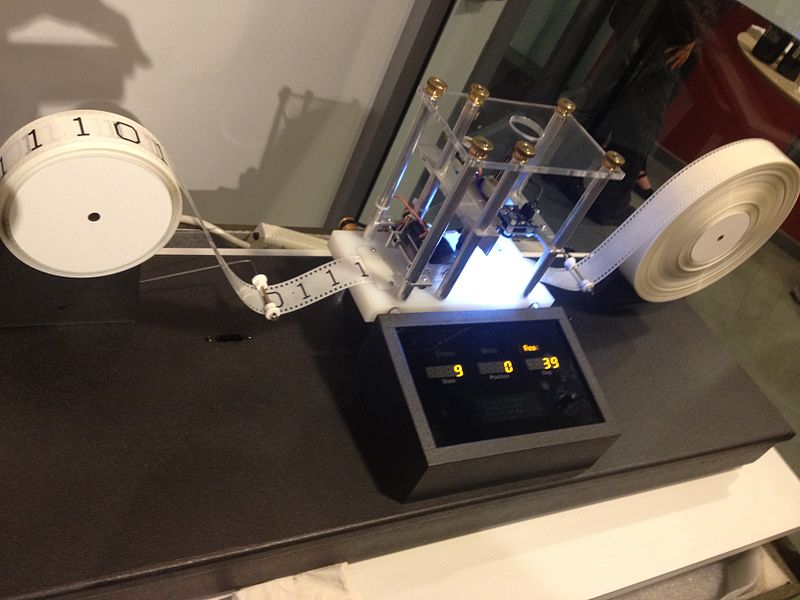
\includegraphics[width=5cm]{turing_machine.jpg}
					\caption{Prototype d'une machine de Turing, source \href{https://commons.wikimedia.org/wiki/File:Model\_of\_a\_Turing\_machine.jpg}{Wikimedia Commons}} merci à GabrielF
				\end{figure}
				La machine commence avec toutes ses cases remplies par des symboles blancs, et dans un état dit initial. A chaque étape qui suit, la tête de lecture lit de contenu de la case sur laquelle elle se trouve, lit son registre et consulte la table pour savoir vers où translater et dans quel état passer. Et ainsi de suite.\\
				Une machine de Turing n'est donc pas si éloignée d'une machine à écrire munie d'un genre de programme d'exécution (la table) et qui pourrait corriger le texte déjà écrit.  
				\begin{eqnarray*}
				(\epsilon, e_I) &\rightarrow& (H, D, e_H)\\
				(\epsilon, e_H) &\rightarrow& (e, D, e_{He}) \\
				\vdots\\
				(\epsilon, e_{Hello}) &\rightarrow& (\epsilon, D, e_{Hello\_})\\
				\vdots\\
				(\epsilon, e_{Hello\_Worl}) &\rightarrow& (d, D, e_F)
				\end{eqnarray*}
				Ci-dessus, une table très simple produisant le texte ``Hello world'' sur la bande, à condition de commencer sur bande vierge, et en supposant que $e_I$ et $e_F$ sont respectivement l'état initial et l'état final de la machine.\\
				
				En informatique, les machines de Turing ne produisent pas directement des caractères; en général, on raisonne sur des machines de Turing définies sur un alphabet trivalent $\lbrace \epsilon, 0, 1 \rbrace$. Notons au passage qu'il s'agit aussi de l'alphabet de Calliope (Section \ref{calliope}), pourvu que l'on identifie le vert avec le $0$, le rouge avec le $1$, et le silence avec $\epsilon$.\\
				Les machines de Turing servent à définir la notion de complexité algorithmique, et la notion d'algorithme tout court~: toute procédure (ou langage) aussi expressif qu'une machine de Turing est considéré comme un algorithme (ou un langage de programmation), et est qualifiée de Turing-complet. Cela dit, la simplicité du modèle et l'atomicité des tâches qui le constituent rendent la génération de texte en langue naturelle relativement complexe. Encore une fois, l'exmple de Calliope montre à quel point l'interprétation de messages binaire est ardue. Aussi, la machine de Turing est davantage un outil théorique que pratique, mais il est intéressant de noter sa capacité à relier l'informatique et la langage naturel au travers de ses spécificités ``mécaniques''.\\
				
				Les automates sont un exemple de théorie plus riche et Turing-complète. Ici le terme peut paraître trompeur, nous ne parlerons pas des automates ``robots'' comme ceux de  Jaquet-Droz~! Pour simplifier, un automate fini est un genre de graphe orienté, composé~:
				\vspace{2mm}
				\begin{itemize}
					\item d'un \textit{input}, qui est une chaîne de symboles. Les symboles sont lus un par un et ``défaussés'' après lecture;
					\item d'états (les nœuds du graphe) en nombre fini. On compte deux types d'états distingués~: l'état initial, et un certain nombre d'états finals\footnote{à noter que cette orthographe n'est pas une coquille};
					\item de transitions (les arêtes du graphe), étiquetées par des symboles. On ne pourra passer d'un état à un autre par une transition que si le symbole lu est une étiquette de cette transition. Autrement dit, l'ensemble des transitions peut être résumé en une table, faisant correspondre à un couple (état, symbole) un état ou plusieurs états (plusieurs dans le cas non-déterministe).
				\end{itemize}
				\vspace{2mm}
				On dit qu'un automate reconnaît un mot (ou plus globalement un langage) lorsque l'exécution de l'automate avec ce mot (ou l'ensemble des mots du langage pris tour à tour) en \textit{input} se termine sur un état final. Un automate pur se prête donc davantage à de la vérification (vérifier que la morphologie d'un mot ou la syntaxe d'une phrase satisfait certains critères de correction) qu'à de la génération.
				\begin{figure}
					\centering
					\begin{tikzpicture}[->,>=stealth',shorten >=1pt,auto,node distance=2.8cm, semithick]
				
						\node[initial,state] (A) {$q_I$};
						\node[state] (B) [right of=A] {$q_b$};
						\node[state, accepting] (C) [right of=B] {$q_c$};
						
						\path
						(A) edge [loop below] node {PREFIX} (A)
						(A) edge node {VS} (B)
						(B) edge node {SUFFIX} (C);
					\end{tikzpicture}
					\caption{Un automate très simple reconnaissant les verbes substantivés comme ``activation'', ``réactivation'', ``réréactivation'', ``désactivation'' etc. (PREFIX = ré$|$dé$|$anti$|$sur... VS = activa$|$consomma$|$constitu... SUFFIX = tion)}
					\label{fig:automata}
				\end{figure}
				Pour aborder la génération, on utilise un outil un peu plus puissant que l'automate, le transducteur. Un transducteur est, de façon très simplifiée, un automate qui en plus de vérifier chaque symbole ``écrit'' un symbole en retour. Les transitions d'un transducteur sont donc étiquetées non plus par un symbole unique, mais par un couple formé du symbole à reconnaître (typiquement, une classe grammaticale, une catégorie de morphème...) et du symbole à retourner (typiquement, un léxème ou un morphème).\\
				\begin{figure}
					\centering
					\begin{tikzpicture}[->,>=stealth',shorten >=1pt,auto,node distance=5.7cm, semithick]
					
					\node[initial,state] (A) {$q_I$};
					\node[state] (B) [right of=A] {$q_b$};
					\node[state, accepting] (C) [right of=B] {$q_c$};
					
					\path
					(A) edge [loop below] node {(PREFIX; ré$|$dé$|$anti$|$sur)} (A)
					(A) edge node {(VS; activa$|$consomma$|$constitu)} (B)
					(B) edge node {(SUFFIX; tion)} (C);
					\end{tikzpicture}
					\caption{Un transducteur générant un verbe substantivé selon le motif abstrait PREFIX* VS SUFFIX}
					\label{fig:transducer}
				\end{figure}
				On voit ainsi que les transducteurs peuvent être le concept sous-jacent à l'idée des ``phrases à trous'' utilisées par Strachey, Lutz et L'OuLiPo. Toutefois les transducteurs gèrent difficilement les conflits liés à la combinatoire. Par exemple, le tranducteur simpliste présenté Figure \ref{fig:transducer} génère des mots corrects comme ``surconsommation'', ``réactivation'', ``constitution'', mais génère aussi une myriade de formes incorrectes comme ``déantiactivation''. La gestion des cas particuliers et des incompatibilités conduit très rapidement à une multiplication des états possibles et des transitions -- ce qui dépasse souvent la capacité humaine. C'est pourquoi des outils comme les transducteurs peuvent difficilement se passer d'une correction manuelle \textit{a posteriori} par l'auteur.
			\subsubsection{Grammaires}\label{grammaires}
				Les grammaires formelles ont des origines très anciennes~: le grammairien indien Panini théorisa le sanskrit à l'aide de ce formalisme dès l'époque antique, même si la présentation était un peu différente de celle utilisée de nos jours.\\
				Mais c'est surtout à Noam Chomsky que l'on doit le développement et la segmentation en différentes catégories de ce formalisme très riche \cite{chomsky1956}. Une grammaire formelle est composée~:
				\vspace{2mm}
				\begin{itemize}
					\item de symboles non-terminaux en nombre fini, qui représentent des catégories abstraites du langage; typiquement, des classes grammaticales, des morphèmes, des catégories de phrases, de compléments ou de propositions.... Il existe un symbole non-terminal distingué appelé $S$, ``racine'' de tous les autres. En général, $S$ désigne une phrase (``\textbf{s}entence'');
					\item de symboles terminaux en nombre fini, qui représentent des parties de l'\textit{output} que l'on désire, typiquement des mots ou plus rarement des portions de phrases;
					\item de règles de production, qui à une chaîne de symboles (terminaux ou non-terminaux) contenant au moins un non-terminal associent d'autres symboles (terminaux ou non-terminaux).
				\end{itemize}
				\vspace{2mm}
				Notons l'importance de la finitude du nombre de symboles. L'idée principale derrière les grammaires formelles était en effet, pour Chomsky, de modéliser un ``système combinatoire discret'' possiblement récursif, et donc capable de générer de l'infini (les phrases) à partir du fini (les symboles). Cette hypothèse est capitale pour un modèle du langage naturel, dans la mesure où le cerveau humain à lui-même une capacité de mémorisation finie; mais que par contre chaque phrase ``non triviale'' que nous prononçons ou écrivons est sans doute prononcée ou écrite pour la première et la dernière fois~!\\
				
				La définition générale des règles de production donnée ci-dessus semble assez complexe. En vérité, des restrictions supplémentaires dans la forme des règles de production donnent lieu à des définitions plus simples de ces règles. Différentes spécifications ``bien choisies'' \footnote{la définition formelle de ces règles plus précises, bien que relativement simple, n'est pas détaillée ici pour des raisons de place} de ces règles de production engendrent alors différentes classes de grammaires, plus ou moins permissives, résumées Figure \ref{fig:chomsky_hierarchy}. C'est ce qu'on appelle aussi la ``hiérarchie de Chomsky''.
				\begin{figure}
					\centering
					\fbox{
						\begin{minipage}{.5\textwidth}
							grammaires générales\\
							~\\
							\fbox{
								\begin{minipage}{.8\textwidth}
									grammaires contextuelles\\
									~\\
									\fbox{
										\begin{minipage}{.8\textwidth}
											grammaires algébriques\\
											~\\
											\fbox{
												\begin{minipage}{.8\textwidth}
													grammaires régulières\\
													~\\
												\end{minipage}}
											\end{minipage}
										}
									\end{minipage}
								}
							\end{minipage}
						}
						\caption{Hiérarchie de Chomsky}
						\label{fig:chomsky_hierarchy}
					\end{figure}
					Pour la génération de langage naturel, les grammaires algébriques (dites aussi ``hors-contexte'') sont généralement utilisées, dans une forme dite ``forme normale de Chomsky''. Les règles de production possibles sont alors beaucoup plus simples\footnote{en réalité, mais pour la forme, il faut ajouter une règle supplémentaire~: la racine$S$ doit pouvoir générer le mot vide $\epsilon$}:
				\vspace{2mm}
				\begin{itemize}
					\item soit un unique non-terminal génère un unique terminal;
					\item soit un unique non-terminal génère exactement deux non-terminaux
				\end{itemize}
				\vspace{2mm}
				Cette forme bien spécifique se comprend bien graphiquement, puisqu'elle donne lieu à une structure arborescente, dont les nœuds internes sont de non-terminaux et dont les feuilles sont des terminaux. Un exemple est donné Figure \ref{fig:ex_syntactic_tree}.
				\begin{figure}
					\centering
					\begin{tikzpicture}
					\Tree [.SENT [.COORD [.VN [.CLS Elle ] [.V était ] ] [.NP [.ADJ pâle ] [.PP [.NP [.AP [.COORD [.CC et ] [.AP [.ADV pourtant ] [.ADJ rose ] ] ] ] ] ] ] ] ]
					\end{tikzpicture}
					\caption[]{Exemple d'arbre généré par une grammaire algébrique. La phrase d'\textit{output} est obtenue en lisant de gauche à droite les feuilles de l'arbre\footnotemark}
					\label{fig:ex_syntactic_tree}
				\end{figure}
				\footnotetext{en fait ici, on a fait l'opération inverse en \textit{parsant} un vers d'un poème de Victor Hugo, à l'aide du \textit{parser} de Stanford disponible ici dans sa version en ligne~: \href{http://nlp.stanford.edu:8080/parser/}{http://nlp.stanford.edu:8080/parser/}. L'approche \textit{bottom-up} est de toute façon équivalente à l'approche \textit{top-down} dans ce genre de formalisme... A noter également que le \textit{parser} de Stanford ne renvoie pas des arbres correspondant à une grammaire en forme normale de Chomsky, dans la mesure ou certains nœuds internes n'ont qu'un seul fils. }
				Les grammaires algébriques sont plus expressives que les automates vus précédemment, mais on pourrait également formaliser les travaux de Strachey, Lutz et certaines contraintes de l'OuLiPo dans ce modèle. A cet égard, les Textes Stochastiques de Theo Lutz ont été traduits par nos soins en une grammaire hors-contexte en Annexe \ref{lutz_grammar}. On pourrait également voir les textes de \textit{Proust Memories} de Jean-Pierre Balpe comme le résultat d'une grammaire dont le terminaux seraient des portions de phrases tirées de \textit{La Recherche} ajoutées à des subordonnants et des conjonctions de coordinations, et dont les seules règles de production seraient des règles de coordination et de subordination.\\
				
				Pour finir sur les grammaires, remarquons simplement que d'autres modèles existent hors de la traditionnelle hiérarchie de Chomsky. Les plus connus seraient peut-être les grammaires transformationnelles \cite{chomsky1979} et les grammaires d'arbre adjoint (TAGs)\cite{joshi1997}.
				
			
		\subsection{Les méthodes statistiques}\label{methodes_stat}
			\begin{citationbox}
				\textit{Nous sommes fatigués de l'arbre. Nous ne devons plus croire aux arbres, aux racines ni aux radicelles, nous en avons trop souffert. Toute la culture arborescente est fondée sur eux, de la biologie à la linguistique. [...] La pensée n'est pas arborescente, et le cerveau n'est pas une matière enracinée ni ramifiée. Ce qu'on appelle à tort  ``dendrites'' n'assurent pas une connexion des neurones dans un tissu continu. La discontinuité des cellules, le rôle des axones, le fonctionnement des synapses, l'existence de micro-fentes synaptiques, le saut de chaque message par-dessus ces fentes, font du cerveau une multiplicité qui baigne, dans son plan de consistance ou dans sa glie, tout un système probabiliste incertain, uncertain nervous system.}
				\begin{flushright}
					Gilles Deleuze et Félix Guattari, \textit{Milles plateaux}, cités par Marine Riguet \cite{riguet2017}
				\end{flushright}
			\end{citationbox} 
			Les méthodes statistiques, se basent de façon peut étonnante sur des statistiques. Or, pour obtenir des statistiques à valeur significative, beaucoup de données \footnote{pour nous, il s'agira de données ``littéraires'' type romans, poèmes... ou bien simplement de données textuelles type journaux, transcriptions de discours...} sont nécessaires. C'est sans doute ce qui explique l'essor tardif des méthodes statistiques par rapport aux méthodes formelles, en effet :
			\vspace{2mm}
			\begin{itemize}
				\item la collecte des données nécessitait de gros volumes de stockage et un stockage performant, mais aussi des moyens de collecte rapides;
				\item le traitement des grands volumes de données nécessitait une grande puissance en matière de processeurs.
			\end{itemize}
			\vspace{2mm}
			Les gros volumes de stockage sont peu à peu devenus accessibles avec la modernisation et la miniaturisation des disques. Aujourd'hui, on peut acheter à moindre frais un disque dur externe d'un Téra, alors qu'il y a dix ans, un disque de 100 Gigas revenait déjà relativement cher. La technologie SSD permet également un accès plus rapide aux données. Pour ce qui est de la collecte des données, on est passé d'un archivage manuel sur cartes perforées (on pense à l'\textit{Index thomisticus} du père Busa, commencé dès 1949...) a un archivage automatique capable de numériser près de 1000 pages par heure (statistiques pour Google Books)\\
			
			Le traitement de ces données massives a été facilité par la loi dite de Moore, qui prédit que le nombre de transistor par processeur (CPU) devrait doubler tous les six mois\footnote{en réalité on sait bien que cette loi devrait converger asymptotiquement vers un valeur limite, la miniaturisation ayant elle-même ses bornes -- celles des effets quantiques...}, augmentant ainsi exponentiellement la puissance de calcul. Mais le progrès le plus notable vient sans doute des cartes graphiques (GPU), qui permettent d'effectuer extrêmement rapidement des calculs spécialisés, en particulier des multiplications de matrices de très grande taille. Les unités de traitement de tenseur (TPU), encore plus performantes car spécialement conçues pour l'apprentissage statistique, devraient très bientôt prendre le relais des GPU (qui au départ servaient au fonctionnement des jeux vidéo...).
			\subsubsection{Chaînes de Markov}\label{markov}
				Les chaînes de Markov ont très tôt été pressenties comme un moyen de générer des suites de mots. Claude Shannon, père de la théorie de l'information, imagine dès 1948 dans \cite{shannon1948} l'utilisation possible de chaînes de Markov simples pour émuler la communication (cela dit ses perspectives n'étaient pas spécialement littéraires). Voici l'un de ses exemples calculés à la main (chaîne de Markov d'ordre $2$):
				\begin{citationbox}
					THE HEAD AND IN FRONTAL ATTACK ON AN ENGLISH WRITER THAT THE CHARACTER OF THIS POINT IS THEREFORE ANOTHER METHOD FOR THE LETTERS THAT THE TIME OF WHO EVER TOLD THE PROBLEM FOR AN UNEXPECTED
					\begin{flushright}
						Claude Shannon, \textit{A Mathematical Theory of Communication} \cite{shannon1948}
					\end{flushright}
				\end{citationbox}
				Au vu de cet exemple, les chaînes de Markov permettent bien de produire des séquences d'éléments avec une certaine cohérence. En effet nous allons voir que chaque nouveau chaînon produit dépend d'un certain nombre de ses prédécesseurs. Dans le cas typique de la génération de texte (comme ci-dessus), la granularité et celle du mot, et le résultat d'une chaîne de Markov est une suite de mots, autrement dit une phrase. Mais le caractère peut aussi être utilisé comme chaînon élémentaires, avec davantage de risques d'incorrections orthographiques, syntaxiques, sémantiques. Dans ce qui suit et pour simplifier, nous garderons le modèle du mot comme chaînon élémentaire.\\
				
				Pour formaliser cette idée, il faut considérer chaque chaînon d'une chaîne de Markov comme une variable aléatoire, pouvant prendre comme valeur n'importe quel mot du dictionnaire\footnote{en pratique on le verra, un ensemble plus réaliste de mots est l'ensemble des mots présents dans le corpus d'entraînement}. On construit la chaîne de Markov en ``tirant'' tour à tour les variables aléatoires qui constituent la chaîne, avec une distribution de probabilité ``conditionnelle'', c'est-à-dire une probabilité qui dépend des tirages déjà effectués. On parle de chaîne de Markov d'ordre $n$ lorsque le tirage de la $k^{eme}$ variable (le $k^{eme}$mot), ne dépend que des $n$ tirages précédents:
				\begin{equation}
					\mathbb{P}[X_{k} = m | X_{k-1} = m_{k-1} \dots X_{0} = m_0] = \mathbb{P}[X_k = m | X_{k-1} = m_{k-1} \dots X_{n+k} = m_{k-n}]
				\end{equation}
				Cette équation suppose un $k \geq n$, autrement dit, la génération ne sera possible qu'avec une chaîne initiale de $n$ caractères, souvent appelée \textit{seed} (graine). Cette chaîne pourra être tirée directement du corpus d'entraînement, ou inventée par l'auteur, comme point de départ de la création.\\
				
				La question qui se pose ensuite est celle des probabilités~: comment évaluer la probabilité de produire un mot en fonction des $n$ mots déjà produits? Cela se fait facilement sur la base d'un corpus d'entraînement. L'idée principale est de regarder toutes les sous-chaînes de longueur $n$ au sein du corpus, et de relever à chaque fois le mot qui suit immédiatement ces chaînes. Pour chaque chaîne, on obtiendra alors une distribution de fréquences des mots suivants, et il suffit alors de normaliser pour obtenir une approximation empirique de la probabilité de transition de la chaîne vers le mot suivant.\\
				
				Par exemple, prenons la chaîne de taille de taille $3$ ``Il prit la'', et cherchons à construire une chaîne de Markov d'ordre $3$. Supposons que notre corpus compte $20$ occurrences de la chaîne ``Il prit la'', dont $10$ occurrences suivies directement de ``parole'', $5$ occurrences suivies directement de ``porte'', et $5$ occurrences suivies directement de ``responsabilité''. On déduira alors que~:
				\begin{eqnarray}
					\mathbb{P}[X_3 = \mbox{``parole''} | X_2 = \mbox{``la''}, X_1 = \mbox{``prit''}, X_0 = \mbox{``Il''}] = \frac{10}{20} = \frac{1}{2}\\
					\mathbb{P}[X_3 = \mbox{``porte''} | X_2 = \mbox{``la''}, X_1 = \mbox{``prit''}, X_0 = \mbox{``Il''}] = \frac{5}{20} = \frac{1}{4}\\
					\mathbb{P}[X_3 = \mbox{``responsabilité''} | X_2 = \mbox{``la''}, X_1 = \mbox{``prit''}, X_0 = \mbox{``Il'}'] = \frac{5}{20} = \frac{1}{4}
				\end{eqnarray}
				
				Un fois que les probabilités ont été calculées à partir du corpus d'entraînement, il est possible de générer du texte. On commence à partir de la graine de $n$ caractères $(m_0, \dots m_{n-1})$ tirée du corpus ou inventée sur le moment, puis on tire au sort le mot suivant selon la distribution donnée par $\mathbb{P}[X_n = m| m_0, \dots m_{n-1}]$. Ce tirage nous donne le mot $m_n$, et il est possible de réitérer un tirage à partir de la chaîne $(m_1, \dots m_n)$ ... et ainsi de suite.\\
				
				Ce modèle qui s'appuie sur les $n$ derniers mots produits peu faire penser à l'écriture automatique des surréalistes. En effet, on a pu voir en Section \ref{ecriture_auto} que lorsque l'on écrit dans un état inconscient, la création se fait le plus souvent par associations d'idées; l'écriture dépend donc de nos dernières pensées. La chaîne de Markov, dont la mémoire est limitée aux derniers mots produits, semble en quelque sorte modéliser cette forme d'écriture spontanée et primesautière. La génération par chaînes de Markov, comme alternative aux méthodes \textit{rule-based} vues précédemment semble réaliser le vœu de Paul Valéry~:
				\begin{citationbox}
					\textit{Peut-être serait-il intéressant de faire une fois une œuvre qui montrerait à chacun de ses nœuds, la diversité qui peut s’y présenter à l’esprit, et parmi laquelle il choisit la suite unique qui sera donnée dans le texte. Ce serait là substituer à l’illusion d’une détermination unique et imitatrice du réel, celle du possible-à-chaque-instant, qui me semble plus véritable.} 
					\begin{flushleft}
						Paul Valéry, \textit{Fragments des mémoires d'un poème}, cité par Philippe Bootz \cite{bootz2012}
					\end{flushleft}
				\end{citationbox}
				
				
			\subsubsection{Le modèle du ``sac de mots continu''}\label{cbow}
				Ce modèle de ``sac de mots'' (en anglais \textit{Continuous Bag of Words}, maintenant CBOW) est assez intéressant dans la mesure où il se fonde sur deux principes qui peuvent sembler orthogonaux~:
				\vspace{2mm}
				\begin{itemize}
					\item une perspective fregeienne, selon laquelle le sens d'un mot dépend du sens des mots qui l'avoisinent et de la manière dont ces mots sont combinés entre eux. C'est ce que l'on appelle aussi le principe de compositionnalité;
					\item une perspective probabiliste ``à la Markov'', la méthode CBOW nécessitant le calcul de probabilités conditionnelles similaires à celles des chaînes de Markov.
				\end{itemize}
				\vspace{2mm}
				Le modèle CBOW permet de générer un mot à partir d'un contexte (les mots qui l'entourent, sur une fenêtre symétrique de taille donnée). Ce modèle se base sur une représentation vectorielle des mots, souvent appelée \textit{embedding}. Faire l'\textit{embedding} d'un mot, c'est trouver sa représentation comme vecteur d'un espace à $n$ dimensions. Pour simplifier, il faut penser les dimensions comme des échelles, ou des caractéristiques spécifiques (par exemple, une dimension pour quantifier la taille, une dimension pour quantifier la couleur...). Un exemple simple d'\textit{embedding} est donné Figure \ref{embedding}. Sans rentrer dans les détails, un \textit{embedding} naïf peut s'obtenir à partir d'une matrice de co-occurrences des mots et d'une décomposition de cette matrice en valeurs singulières \cite{socher2016}.
				\begin{figure}
					\centering
					\begin{tikzpicture}
				\begin{axis}[
				enlargelimits=true,
				ylabel=Intensité,
				xlabel=Registre,
				]
				\addplot+[
				nodes near coords,only marks,
				point meta=explicit symbolic]
				table[meta=Mot]
				{
					Registre Intensite Mot
					.9 .9 ``Grandiose''
					.2 .2 ``Nul''
					.1 .2 ``Moche''
					.7 .8 ``Superbe''
					.7 .85 ``Magnifique''
					.7 .3 ``Laid''
					.3 .5 ``Beau''
					.7 .1 ``Ignoble''
					.1 .1 ``Dégueu''
					.1 .6 ``Stylé''
				};
				\end{axis}
				\end{tikzpicture}
				\caption{Exemple naïf d'\textit{embedding} à deux dimensions pour des adjectifs appréciatifs}
				\label{embedding}
				\end{figure}
				L'idée derrière le modèle CBOW est~:
				\vspace{2mm}
				\begin{itemize}
					\item d'encoder en \textit{one-hot} les mots du contexte. Un encodage one-hot transforme un mot issu d'un lexique de taille $N$ en un vecteur de taille $N$, possédant une seule coordonnée à $1$ (celle que l'on a choisie pour ``correspondre'' au mot) et les autres coordonnées à $0$;
					\item de transcrire les vecteurs one-hot dans l'\textit{embedding}, à l'aide d'une matrice d'\textit{embedding};
					\item calculer le barycentre (somme pondérée) de ces vecteurs (c'est l'application du principe de compositionnalité);
					\item de donner un score à ce barycentre (via une multiplication matricielle), puis transformer ce score en vecteur de probabilités à l'aide d'un \textit{softmax}
				\end{itemize}
				\vspace{2mm}
				Le vecteur de probabilités qui résulte de cette méthode donne, pour chaque mot du lexique, la probabilité d'avoir ce mot sachant le contexte. Il s'agit donc de probabilités conditionnelles comme dans le cas des chaînes de Markov.\\
				
				Il est à noter que les matrices d'\textit{embedding} et de score sont ``apprises'' sur un corpus~: le mot central et son contexte sont alors connus, et le ``vrai'' mot central est comparé avec l'\textit{output} du système. Les fonctions d'\textit{embedding} et de score sont alors corrigées en vue de minimiser une fonction objectif (de type entropique), avec des algorithmes classiques d'optimisation. Mais pour des raisons d'espace (et de complexité) nous n'allons pas rentrer dans ces subtilités. \\
				
				Ce qu'il faut retenir de cette méthode est la représentation vectorielle des mots, et l'approche très géométrique de ce qu'est la signification (un barycentre~!). Un autre élément frappant est la totale ignorance du système des règles syntaxiques et des interactions qu'ont les mots entre eux. La phrase est relativement dévoyée, elle est considérée comme un ``sac'' et seules les co-occurences des mots en son sein comptent. Malgré cela la méthode CBOW a fait ses preuves sur des corpus variés. Cela pose la question de la connaissance qu'à le système des entités manipulées par rapport au résultat final obtenu, mais nous y reviendrons en Section \ref{nouvelle_definition}.
			\subsubsection{Les réseaux de neurones}\label{neural_net}
				\subsubsubsection{Présentation générale}
					Les réseaux de neurones sont sans doute le fer de lance de l'intelligence artificielle à l'heure actuelle. Inspirés de la philosophie connexionniste\footnote{le connexionnisme est apparu dans les années 80 comme une alternative au computationnalisme. L'approche connexionniste conçoit les phénomènes mentaux comme des processus émergents qui résultent de l'interconnexion d'éléments simples, typiquement des ``neurones''.} et du biomimétisme, ils sont les premiers modèles à réellement invalider la thèse de Philippe Bootz dans~:
					\begin{citationbox}
						\textit{[l'intelligence artificielle] simule le produit créatif, non le processus créatif.}
						\begin{flushright}
							Phillipe Bootz, \textit{Un historique de la génération numérique de textes} \cite{bootz2006}
						\end{flushright}
					\end{citationbox}
					...si bien sûr on assimile le comportement de nos neurones à nos mouvements créatifs.\\
					En effet, le modèle sous-jacent aux réseaux de neurones s'inspire fortement de l'architecture du système neuronal chez l'humain et les autres mammifères. Chaque neurone d'un réseau de neurones intègre les informations transmises pas d'autres neurones (en leur attribuant un certain \textit{poids}), et transmet à son tour des informations à ses voisins. Les réseaux de neurones sont organisés en \textit{couches} auxquelles correspond en théorie un niveau d'abstraction particulier\footnote{l'idée derrière cette interprétation vient encore une fois des sciences cognitives, et en particulier de la reconnaissance d'objets~: lorsque l'on cherche à identifier un objet, on s'arrête d'abord sur les caractéristiques globales (taille, forme, contours...), puis on se penche sur des caractéristiques plus précises (texture, détails particuliers, parties de l'objet...). Les premières couches d'un réseau de neurones devraient ainsi s'attacher aux caractéristiques globales, tandis que les dernières couches se porteraient sur les points de détail.}. Pour nous, le ``niveau d'abstraction'' sera celui des caractères, des syllabes, des mots ou des phrases, même si bien évidemment la segmentation opérée par la machine -- qui on le rappelle est non supervisée, sans règles \textit{a priori} sur ce qu'est un mot, une phrase... -- peut varier par rapport à l'interprétation humaine.
					\begin{figure}
						\centering
						\def\layersep{3.5cm}
						\begin{tikzpicture}[shorten >=1pt,->,draw, node distance=\layersep]
						\tikzstyle{every pin edge}=[<-,shorten <=1pt]
						\tikzstyle{neuron}=[circle,minimum size=17pt,inner sep=0pt, draw]
						\tikzstyle{input neuron}=[neuron];
						\tikzstyle{output neuron}=[neuron];
						\tikzstyle{hidden neuron}=[neuron];
						\tikzstyle{annot} = [text width=10em, text centered]
						
						% Draw the input layer nodes
						\foreach \name / \y in {1,...,4}
						% This is the same as writing \foreach \name / \y in {1/1,2/2,3/3,4/4}
						\node[input neuron, pin=left:] (I-\name) at (0,-\y) {};
						
						% Draw the hidden layer nodes
						\foreach \name / \y in {1,...,5}
						\path[yshift=0.5cm]
						node[hidden neuron] (H-\name) at (\layersep,-\y cm) {};
						
						% Draw the output layer node
						\node[output neuron,pin={[pin edge={->}]right:Output}, right of=H-3] (O) {};
						
						% Connect every node in the input layer with every node in the
						% hidden layer.
						\foreach \source in {1,...,4}
						\foreach \dest in {1,...,5}
						\path (I-\source) edge (H-\dest);
						
						% Connect every node in the hidden layer with the output layer
						\foreach \source in {1,...,5}
						\path (H-\source) edge (O);
						
						% Annotate the layers
						\node[annot,above of=H-1, node distance=1cm] (hl) {Deuxième couche (couche \textit{cachée})};
						\node[annot,left of=hl] {Première couche (couche \textit{input})};
						\node[annot,right of=hl] {Dernière couche (couche \textit{output})};
						\node[annot,left of=I-2, rotate=90] {Input};
						\end{tikzpicture}
						\caption{Un réseau de neurones simple a $3$ couches. Chaque cercle est un neurone, les arc entre les cercle sont des ``synapses''}
						\label{fig:neural_net}
					\end{figure}
					La couche d'\textit{input} d'un réseau de neurones prend comme entrée un vecteur. Chaque composante scalaire du vecteur entre dans un neurone (un cercle sur la Figure \ref{fig:neural_net}).\\
					Ensuite, le passage d'une couche quelconque $n$ à un neurone $i$ de la couche suivante ($n+1$) se fait en plusieurs étapes~:
					\vspace{2mm}
					\begin{itemize}
						\item les valeurs des neurones de la couche $n$ sont pondérées (c'est-à-dire multipliées chacune par un poids scalaire différent et dépendant du neurone $j$ considéré);
						\item les valeurs pondérées sont combinées entre elles, par exemple en faisant un somme;
						\item la valeur ainsi obtenue subit éventuellement une non-linéarité (seuil, softmax, ReLu...)
					\end{itemize}
					\vspace{2mm}
					Ce procédé est répété individuellement pour chaque neurone de la couche $n+1$\\
					La dernière couche compte autant de neurones que le vecteur d'\textit{output} à de dimensions. Si l'on se rappelle l'\textit{embedding} simpliste à deux dimensions de la Figure \ref{embedding}, un réseau de neurones qui aurait généré cet \textit{embedding} aurait eu une deuxième couche composée de deux neurones (donc deux ``cercles''). Le passage de la dernière couche au vecteur d'\textit{output} se fait souvent avec une non-linéarité type softmax ou ReLu, accompagnée éventuellement d'un peu d'échantillonnage.\\
					
					L'élément ``apprenant'' du réseau de neurones, ce sont ses poids, autrement dit la pondération associée à chacun de ses arcs. Ces poids sont peu à peu modifiés au fur et à mesure de l'entraînement sur un corpus. La modification s'opère suivant un algorithme bien connu appelé ``\textit{backpropagation}''. Cet algorithme consiste grossièrement à~:
					\vspace{2mm}
					\begin{itemize}
						\item comparer l'\textit{output} du réseau de neurones avec la valeur attendue (on rappelle que l'entraînement se fait sur un corpus où les ``vrais'' résultats sont connus). Cela se fait souvent à  l'aide d'une fonction d'entropie croisée, inspirée de la théorie de l'information. La fonction va renvoyer une valeur quantifiant l'écart entre la valeur de l'\textit{output} et la ``vraie'' valeur.
						\item répercuter le delta entre l'\textit{output} et la ``vraie'' valeur sur les poids du réseau, en ``pénalisant'' les neurones qui seraient responsables de l'erreur. C'est à cette étape que l'on rebrousse chemin dans le réseau et corrigeant les neurones à la volée.
					\end{itemize}
					\vspace{2mm}
					En temps normal, les poids du système finissent par converger vers une valeur stable. Mais pour les réseaux de neurones en général, les garanties de convergence demeurent très faibles et l'on ne peut même pas savoir si le réseau de neurone à réellement convergé vers ce que l'on juge être la ``bonne interprétation'' (un \textit{optimum global}).
				\subsubsubsection{Le cas particulier des réseaux LSTM, et une courte simulation}\label{lstm_hugo}
					En génération de texte, une catégorie bien précise de réseaux de neurones est utilisée. Il s'agit des réseaux LSTM (\textit{Long short-term memory}) qui simulent l'attention humaine face au contexte (ce qui implique des ``oublis'' par exemple). Une schéma de ce réseau de neurones particulier est donnée Figure \ref{fig:lstm}
					\begin{figure}
						\centering
						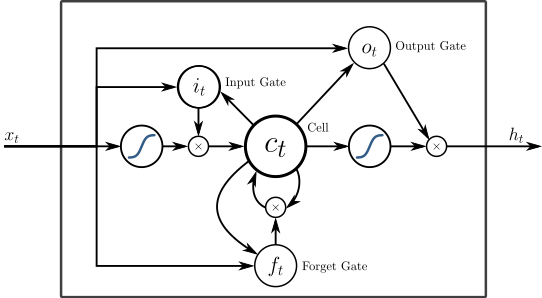
\includegraphics[width=7cm]{lstm.png}
						\caption{Schéma d'un réseau LSTM}
						\label{fig:lstm}
					\end{figure}
					C'est ce type de réseau que nous avons choisi d'utiliser pour une très courte simulation des capacités des réseaux de neurones en termes d'imitation de style. Nous avons utilisé un code d'exemple de la bibliothèque de \textit{deep learning} Keras\footnote{code accessible sur \href{https://github.com/keras-team/keras/blob/master/examples/lstm_text_generation.py}{https://github.com/keras-team/keras/blob/master/examples/lstm\_text\_generation.py}} pour générer des poèmes épiques ``dans le style de Victor Hugo'' caractère par caractère. Ce petit projet consistait à~:
					\vspace{2mm}
					\begin{itemize}
						\item récupérer un corpus d'entraînement composé de poèmes épiques de Victor Hugo sur le site du Projet Gutenberg \href{http://www.gutenberg.org/}{http://www.gutenberg.org/}. Nous avons choisi le recueil \textit{La Légende des Siècles};
						\item entraîner le réseau à prédire le prochain caractère sur la base de morceaux de texte longs de $40$ caractères tirés du corpus;
						\item à partir d'une \textit{seed} tirée au hasard dans \textit{La Légende des Siècles}, générer à la volée les caractères suivants en utilisant le modèle préalablement entraîné.
					\end{itemize}
					\vspace{2mm}
					L'``inventivité'' du système au moment de la génération est paramétrée par une variable appelée \textit{diversity}. Cette ``diversité'' ajoute en fait du bruit au moment du choix du caractère suivant. Plus la diversité est grande, plus le réseau de neurones sera susceptible de générer un caractère ``moins probable'' selon ses propres calculs. La ``diversité'' est donc un facteur de sérendipité. Sans ``diversité'', le réseau de neurones choisit systématiquement le caractère qu'il juge le plus probable entre tous, ce qui donne souvent lieu à des boucles infinies, où la même séquence de caractères revient invariablement, comme si l'IA ``bégayait''.\\
					
					Des exemples d'exécution de notre générateur à base de LSTM sont donnés en Annexe \ref{lstm_hugo_ex}. Nous avons retenu dans l'Annexe le paramétrage du modèle qui a donné la meilleure performance  au cours de l'entrainement (\textit{loss} la plus faible). Différents niveaux de diversité ont été testés sur ce modèle.\\
					
					La première chose qui frappe au vu des résultats est la différence entre le peu de structure de l'\textit{input} (de simples caractères, même pas des mots, et encore moins des vers), et la structuration générale de l'\textit{output}, qui ressemble globalement à un poème. Le système a compris seul qu'il fallait régulièrement segmenter les chaînes de caractères avec des espaces pour former des mots, que les mots étaient séparés par de la ponctuation et qu'il fallait retourner à la ligne assez souvent pour former des vers.\\
					
					Outre la structure, le réseau de neurones a généré du contenu. Certes, les mots générés ne sont pas tous des mots du français, mais globalement, leur forme fait sentir qu'ils \textit{pourraient} faire partie de la langue. Chose étonnante à ce sujet, certains mots inventés par le système font curieusement penser à des mots de proto-français ou d'ancien français. Ci-dessous, quelques néologismes ``élégants'' ont été recopiés~:
					\begin{citationbox}
						\textit{marquisant}\\
						\textit{ouseaux}\\
						\textit{étoileau}\\
						\textit{calpette}\\
						\textit{hétillée}\\
						\textit{frazilla}\\
						\textit{tristercie}\\
						\textit{comtonnête}\\
						\textit{gouffresiches}\\
						\textit{pétilles}\\
					\end{citationbox}
					En regardant ces exemples, on pourrait presque croire que le système a de lui même crée des mots-valise (notamment : \textit{comtonnête} qui fait penser à \textit{comte} \textit{honnête} !). L'inventivité lexicale du modèle est donc assez surprenante, et celle-ci va croissant avec le niveau de sérendipité.\\
					
					Pour ce qui est de la syntaxe, le système semble pouvoir en imiter les rudiments. En particulier, il semble porter son dévolu sur la coordination et le complément du nom, deux structure extrêmement simples; les compositions impliquant des verbes conjugués sont en revanche délaissées (le système doit mal gérer les dépendances dites \textit{à longue distance}...). De plus le système semble avoir ``compris'' qu'en moyenne il y a coïncidence entre un unité syntaxique et un vers; ainsi beaucoup de vers produits se terminent par un signe de ponctuation.\\
					
					Ce petit exemple doit être vu comme une ``preuve de concept'' que les réseau neuronaux sont capables de produire à moindres frais (le code est très court, et relativement simple) des poèmes amusants même si la gestion de la sémantique laisse à désirer.
					
		\subsection{Synthèse}
			Dans cette partie, nous avons pu relier plus précisément les œuvres historiques d'auteurs comme Christopher Strachey, Theo Lutz, Jean-Pierre Balpe et même les surréalistes... rencontrés en Section \ref{genealogie}, avec des concepts mathématiques situés aux fondements de l'informatique moderne, mais aussi avec des méthodes statistiques, plus récentes, vertigineuses par leur simplicité et leur efficacité. Mais dans ce cas, à quel dieu se vouer~? Celui des méthodes formelles et symboliques, ou celui des méthodes statistiques~?\\
				
			Les méthodes formelles à base de grammaires et d'automates peuvent paraître à bien des égards trop simplistes pour le traitement du langage naturel, à la fois infiniment plus riche que les langages de programmation (qui étaient la première application de ces méthodes), et très souvent ambigu (au niveau sémantique comme au niveau syntaxique...). Cela dit, des modèles enrichis existent aujourd'hui \footnote{on pense par exemple aux ``grammaires syntagmatiques guidée par les têtes'', en anglais \textit{head-driven phrase structure grammars}, qui intègrent en une seule structure tous les niveaux linguistiques, de la phonétique à la sémantique}, mais au prix d'un nombre de règles très important et d'un complexité de traitement accrue. La capacité humaine aurait bien du mal à formaliser de cette façon la totalité des règles régissant un langage, jusqu'aux aspects les plus irrégulier et idiomatiques.
			
			\begin{citationbox}
				\textit{les moteurs de règles sont beaucoup trop simplistes pour donner du sens à la complexité. La vie est bien plus complexe que de simples énoncés de règles, ou alors les règles se contredisent et la machine bugge.}
				\begin{flushright}
					Gilles Moyse, \textit{Entretien pour la revue Usbek et Rica} \cite{edin2018}
				\end{flushright}
			\end{citationbox}
			
			
			Or ce sont souvent ces aspects qui sont les plus recherchés en création littéraire. Il semblerait donc que de par leur structure même, les modèles \textit{rule-based} soient inadaptés à la génération de textes originaux. En revanche, ces méthodes se révèlent très robustes et performantes dans des domaines très circonscrits, où l'usage de la langue s'écarte peu des cannons attendus et définis au travers des règles passées au système. Le système produira alors des  énoncés conformes et cette capacité à produire des énoncés conforme sera \textit{prouvable}, car le modèle est en quelque sorte construit sur un schéma d'axiomes.\\
				
			Les méthodes statistiques maintenant, paraissent à l'heure actuelle beaucoup plus alléchantes. Elles permettent en effet à l'humain de déléguer beaucoup plus de prérogatives à la machine, qui choisit elle-même quelles ``règles''\footnote{on ne peut pas vraiment parler de règles au sens strict, mais plutôt de directives suivies ``la plupart du temps''...} se donner, sur quelles caractéristiques porter son ``attention''\footnote{une branche du \textit{machine learning}, très porteuse actuellement, et même spécialisée dans ce que l'on appelle les mécanismes d'attention, ou \textit{attention mechanisms}}, quels motifs intégrer et à quelle échelle etc. On arrive même aujourd'hui à reproduire l'hypothèse dite de la pauvreté du stimulus linguistique sur des machines, avec des modèles statistiques qui n'ont plus besoin que de quelques exemples pour apprendre un maximum sur leur \textit{input} (modèles faiblement supervisés, \textit{zero shot learning}...). Tout cela porterait à croire que les modèles statistiques sont véritablement propres à simuler le langage humain, tant dans le processus que dans le résultat. Néanmoins, il convient de tempérer cette affirmation; car le grand problème des méthodes statistiques à l'heure actuelle, c'est sans doute l'inconnaissance que nous en avons. Comme le dit Anaïs Guilet, les états intermédiaires des réseaux de neurones sont une énigme pour le programmeur, et par conséquent, aucune garantie sur le résultat ne peut être à ce jour donnée~:
			\begin{citationbox}
				\textit{Complexes à implémenter, les RNN offusquent également ces états invisibles par lesquels l'apprentissage artificiel transite.}
				\begin{flushright}
					Anaïs Guilet et Franck Soudan, \textit{Robopoïèse} \cite{guilet2017}
				\end{flushright}
			\end{citationbox}
			\begin{citationbox}
				\textit{La question se transforme quand on se trouve dans l’incapacité d’expliquer dans le détail un processus comme le deep learning. Dans ce cas précis, le résultat semble satisfaisant et on sait comment on a mis en œuvre le dispositif mais on ne sait pas comment cela fonctionne dans la ``boîte noire''. S’il y a un enjeu de savoir, cela tient au fait qu’il peut paraître étrange que la production du savoir puisse être un phénomène obscur. Il est pourtant fondamental de savoir et comprendre, selon quelles instructions un logiciel, qui suit des instructions précises, aboutit à une conclusion, prend une décision, procède à un arbitrage, etc.}
				\begin{flushright}
					Gilles Moyse, \textit{Entretien pour la revue Usbek et Rica} \cite{edin2018}
				\end{flushright}
			\end{citationbox}
			Seul un constat empirique permet de statuer qu'effectivement, ce genre de méthode fonctionne, et même, fonctionne très bien. Mais n'est-ce pas problématique lorsque l'on cherche à générer un texte littéraire~? En délégant ses responsabilités au moment de la génération, l'auteur-programmeur s'engage en quelque sorte à une relecture de l'œuvre \textit{a posteriori}, pour y déceler fautes d'orthographe, incompatibilités lexicales ou faux-sens gênants. Mais d'un autre côté (et nous le verrons plus en détails dans la section suivante), certaines imperfections de la machines peuvent être considérées comme une forme de créativité que les méthodes \textit{rule-based} sont incapables de manifester.\\
			
			En somme, si la complexité des systèmes \textit{rule-based} semble balayée par la simplicité des modèles statistiques, la question des garanties du système elle, est complètement évacuée par la plupart des méthodes modernes. Mais la correction et la conformité à la norme linguistique sont-elles réellement des données à prendre en compte~? Ne serait-ce pas là rester dans un paradigme littéraire antérieur à l'apparition des ordinateurs~? Ne serait-ce pas là dénier \textit{de facto} toute capacité de création de la part de la machine~?
		\newpage
	\section{Vers une nouvelle définition de la littérature}\label{nouvelle_definition}
		Dans les sections précédentes, nous avons eu l'occasion de rencontrer des exemples divers de ce que nous avons choisi d'appeler  ``littérature générative''. Nous avons aussi pu voir que leur degré de complexité ont varié~: de la combinatoire, aux réseaux de neurones récurrents, en passant par les modèles à trous, les grammaires génératives etc.
		Mais nous n'avons pas encore discuté d'un point pourtant crucial dans cette affaire, qui concerne l'ensemble des effets produit par ces littératures et des répercussions possibles sur la notion même de littérature. Nous pouvons dégager deux types d'effets~:
		\vspace{2mm}
		\begin{itemize}
			\item un effet ``d'inquiétante similarité'', lorsque le texte ressemble à s'y méprendre à un texte écrit par un auteur humain;
			\item un effet ``d'inquiétante étrangeté''\footnote{nous reprenons ici librement un terme associé au lexique freudien (ou même antérieur, au romantisme allemand), car nous pensons qu'effectivement la littérature générative peut dans certains cas faire état d'un ``retour inquiétant du même'', et peut engendrer une certaine anxiété chez le lecteur.}, lorsque le texte assume son côté ``robotique'' et semble développer son langage propre, sa propre logique poétique.
		\end{itemize}
		\vspace{2mm}
		Le premier point nous le verrons, repose la question de la place de l'auteur et de l'attribution des textes, un problème déjà bien connu en théorie littéraire. Le second point pose davantage la question du langage poétique et de nos standards esthétiques en la matière, à un moment où les auteurs, dans une dynamique en quelque sorte inverse, tendent à écrire des œuvres de plus en plus ``synthétiques'' (au sens d'artificiel, non-humain).\\
		Comment donc définir une ligne de démarcation entre la littérature ``humaine'' et la littérature ``non-humaine'' lorsque les deux catégories s'empruntent réciproquement leurs codes distinctifs ? Et, de façon plus cruciale encore, existe-t-il vraiment une différence de nature entre ces deux littératures qui justifierait une telle discrimination ? Car, comme le rappelle Anaïs Guilet~:
		\begin{citationbox}
			\textit{Composante essentielle du transhumanisme, si les I.A. produisent indéniablement de nouveaux effets, elles bouleversent également l'approche logique de l'information (connexionniste) ainsi que la conception (presque phénoménologique) des programmes.}
			\begin{flushright}
				Anaïs Guilet et Franck Soudan, \textit{Robopoïèse} \cite{guilet2017}
			\end{flushright}
		\end{citationbox}
		Nous essaierons de répondre à ces questions en convoquant les exemples historiques déjà mentionnés, mais aussi en nous appuyant sur des fictions récentes traitant elles-mêmes à leur manière de cette problématique. A noter également que cette section développera une discussion autour de l'IA vue comme un modèle statistique (réseaux de neurones etc.). Les sytèmes \textit{rule-based}, plus anciens et un peu délaissés actuellement, ne seront pas au centre des interrogations de ce chapitre.
		\subsection{Inquiétante similarité~: la question de l'attribution}
			Les IAs, toujours plus complexes, arrivent de mieux en mieux à imiter le langage humain en littérature, mais s'appuient aussi de plus en plus sur le \textit{big data}, autrement dit, d'immenses corpus littéraires. Faut-il donc attribuer le succès des IAs à leur seul ``mérite''? Faut-il y voir au contraire les talents et l'ingéniosité du programmeur~? Ou bien, les capacités des IAs sont-elles désormais totalement vides et entièrement volées aux écrivains des corpus littéraires sur lesquels elles s'appuient~?
			\subsubsection{La capacité des machines à imiter, entre fiction et réalité}\label{fiction_vs_realite}
				Certaines œuvres, en particulier les œuvres contemporaines utilisant des méthodes d'apprentissage statistique sophistiquées et s'appuyant sur de très grands corpus de données, sont aujourd'hui susceptibles de berner un lecteur humain, qui croit lire la production d'un auteur moderne. Nous donnons ici quelques exemples frappants de ``confusion'' (ou à tout le moins, de traitement égal) entre l'authentique et le synthétique.
				\subsubsubsection{Dans la fiction : des capacités fantasmées}
					Les exemples fictionnels d'IAs réellement ``intelligentes'' sont évidemment très nombreux. Nous comparerons dans cette section l'IA-écrivain Ada du roman éponyme d'Antoine Bello \cite{bello2016} et les androïdes de la série télévisée \textit{Westworld} de Jonathan Nolan et Lisa Joy \cite{westworld}.\\
					
					La première observation face aux contenus fictionnels que l'on s'est proposé d'aborder, c'est la très forte ressemblance entre les machines et les humains; cette ressemblance est beaucoup plus forte que dans la réalité actuelle. Dans le série \textit{Westworld}, les personnages robotiques sont joués par des humains, donc sont \textit{de facto} physiquement indiscernables par rapport aux humains. Ils s'expriment aussi d'une façon sensiblement identique, usent de métaphores et développent des raisonnements profonds. Dans une scène connue de la série, le responsable informatique (Bernard) qui croit s'entretenir avec une androïde (Dolores) afin de diagnostiquer ses bugs, se retrouve en fait lui-même diagnostiqué par sa patiente, car il se révèle être lui aussi un robot.\\
					
					Il en va de même dans \textit{Ada} d'Antoine Bello~: même si dans ce roman l'IA n'est pas incarnée, son langage est bien au-dessus de l'état de l'art actuel en terme de génération de texte. Elle est capable d'humour, de complicité, et elle est susceptible de mentir de façon convaincante -- autant de capacités qui sont aujourd’hui au centre des recherches en matière d'IA. Pourtant (et cela est un peu étrange), Ada n'est pas capable d'écrire de bons romans, alors que cela est censé être sa mission dans l'intrigue\footnote{savoir si Ada parvient à produire une œuvre littéraire à l'issue du roman dépend des interprétations. Le fin du roman laisse en effet entendre que, soit le roman lui-même est l'œuvre d'Ada, auquel cas l'IA aurait bel et bien réussi à produire une œuvre originale; soit le roman est en fait l'œuvre du héros Frank, auquel cas Ada aurait échoué dans son entreprise.}; mais il faut tout de même saluer sa capacité à monter un scénario entier avec des personnages et un fil conducteur (cf. Annexe \ref{ada_elaboration}). Malgré la mièvrerie de la production (qui d'ailleurs est relativement imposée à Ada) on dépasse encore clairement le niveau actuel de la recherche en matière de génération de textes littéraires...\\
					
					Toutefois une question peut-être plus cruciale vis-à-vis de ces représentations fictionnelles de l'IA serait peut-être~: y a-t-il une conscience derrière les calculs~? En effet, et nous le verrons plus en détails dans la Section \ref{test_turing}, une parfaite correction linguistique n'implique pas forcément une véritable conscience littéraire.\\
					
					Dans le cas d'\textit{Ada}, la machine semble ainsi avoir un réelle compréhension de la syntaxe, de la sémantique, et des processus littéraires en général. Ada est même capable sans le savoir d'écrire un vers de haïku identique à celui qu'un auteur humain avait imaginé des années auparavant. Cependant, l'IA n'arrive pas à traduire en mots le véritable sentiment amoureux, un sentiment qui lui semble inaccessible (cf. Annexe \ref{ada_phenomenologie}). La rhétorique mise en place dans \textit{Ada} reprend en quelque sorte celle de Frank Jackson dans son expérience de pensée en faveur du ``\textit{knowledge argument}'', intitulée ``\textit{Mary the super-scientist}'' \cite{jackson1982}. Ce raisonnement tend à dire que, même si l'on possède toutes les informations théoriques sur un concept phénoménologique (comme Ada, qui sait tout sur le sentiment amoureux grâce à Internet), rien ne remplace l'expérience vécue de ce concept. Or, Antoine Bello tend dire qu'un telle expérience vécue est réservée aux êtres de chair.\\
					
					Dans \textit{Westworld} au contraire, les robots même s'ils ne sont pas écrivains, semblent avoir (pour certains) une véritable conscience derrière (ou au sein de) leur algorithme. Ils peuvent avoir un coup de foudre, ressentir de l'amour filial. La série semble supporter l'idée selon laquelle un programme parfait serait capable d'émuler voire de dépasser les capacités humaines en termes de sentiments comme en termes d'expression et de comportement.\\
					
					Ces deux fictions qui jouent à l'envi avec le test de Turing (cf. Section \ref{test_turing}), mettent donc un point d'honneur à brouiller les pistes entre l'humain et le non humain, en donnant un vision sans aucun doute très prospective de ce qu'est un androïde doté de parole.
					
					
					%Elle veut écrire Raison	 et	 sentiments,	Les	 Hauts	 de Hurlevent,	Anna	 Karenine p.93
					%Franck finit par touver dans un poème de ahikus un vers qu'ada avait aussi composé et qu'il avait trouvé affreux	p199
					%ada : contrasate entre la production de la machine et celle de franck (les haïkus, simplicité irréductible)
					%ada : dysfonctionnements lexicaux
					
				\subsubsubsection{Dans la réalité~: importance de l'intervention humaine}
					Au travers des exemples réels qui suivent, nous verrons que l'IA est loin d'être aussi avancée que le prétendent les fictions, et par ailleurs que l'auteur (ou plus généralement l'humain) occupe une place de plus en plus ambiguë dans le processus de création. Nous étudierons deux exemples~: celui d'un livre japonais ``écrit'' par un robot (qui fait écho au roman à l'eau de rose écrit par Ada), et celui d'un scénario de film également écrit par une IA.\\
					
					En 2016 au Japon, un livre ``écrit'' par une intelligence artificielle a failli remporter un prix littéraire de science-fiction, le \textit{Hoshi Shinichi Literary Award}. Cet auteur robotique, développé par l'équipe d'Hitoshi Masuraba de la Future University d'Hakodate, a réussi à se démarquer des 1450 autres participants (dont 11 autres robots) avec son livre au titre évocateur~: \textit{Le jour où un ordinateur écrit un roman}. Cette performance est d'autant plus remarquable que le jury n'était pas informé de l'origine des textes (humaine ou informatique). Ci-dessous, les dernières lignes du roman en question~:
					\begin{citationbox}
						\textit{Je frémissais de joie, que je ressentais pour la première fois, et je continuais à écrire avec entrain. Le jour où un ordinateur a écrit un roman. L'ordinateur décida de se concentrer sur la poursuite de sa propre joie et arrêta de travailler pour les humains.}
						\begin{flushright}
							\textit{Le jour où un ordinateur écrit un roman}
						\end{flushright}
					\end{citationbox}
					Ce passage est relativement \textit{bluffant}. Toutefois, même si la dernière phrase semble faire écho aux thématiques d'Ada (ordinateur qui s'échappe pour écrire par lui-même son propre chef-d'œuvre), force est de constater que l'influence de l'humain a été beaucoup plus déterminante dans la rédaction du roman japonais.\\
					En réalité, les scientifiques avaient le contrôle sur un certain nombre de paramètres du roman, comme la ``trame narrative'' et le genre des personnages. De plus, l'algorithme aurait davantage ``sélectionné'' des mots et des phrases préparées par des humains qu'écrit lui-même l'intégralité de l'histoire (en partant simplement d'un jeu de caractères ou de mots, par exemples). En effet, l'écriture du roman par l'algorithme nécessitait un ``roman modèle'', écrit cette fois-ci par des humains. En prenant en compte l'ensemble de ces informations, l'intelligence artificielle n'aurait réellement ``écrit'' que 20\% de l'histoire\footnote{le mode de calcul de ce pourcentage gagnerait à être explicité dans nos sources}...\\
					
					Cela dit, Satoshi Hase, un romancier japonais qui a pris la parole à la conférence de presse du concours, a avoué avoir été ``surpris du travail, car c'est un roman très structuré. Même s'il reste quelques problèmes à corriger avant qu'il puisse gagner le prix, comme la description des personnages''. L'ordinateur a donc réussi à construire du sens ; et paradoxalement, c'est plus son manque de créativité, d'originalité, d'audace peut-être, qui aurait pénalisé sa production. L'IA a  semble-t-il imité trop platement son modèle...ce qui pose la question de la vacuité de la notion d'auteur dans le cas des productions d'IAs. Mais nous reviendrons sur ce problème et sur celui de l'imitation en général Section \ref{place_auteur} et Section \ref{test_turing}.\\
					
					Le script de \textit{Sunspring} et son interprétation \cite{sunspring} posent le problème de l'attribution d'une façon sans doute plus subtile. \textit{Sunspring} est en effet un court métrage de science fiction expérimental \textit{entièrement} écrit par une intelligence artificielle à l'aide de réseaux de neurones récurrents adaptés à la génération de texte (LSTM, cf. Section \ref{neural_net}). Le film avait originellement été crée pour un challenge de 48 heures organisé par le festival \textit{Sci-Fi-London}, où il a fini dans le top 10 sur plusieurs centaines de participants. Le film a par la suite été mis en ligne par \textit{Ars Technica}, en juin 2016. Nous avons également eu l'occasion d'en voir un extrait lors de l'exposition \textit{Artistes et Robots} au Grand Palais (printemps 2018) \cite{artistes_robots}.\\
					
					L'idée est due à Oscar Sharp, un cinéaste britannique qui a réalisé le film avec l'aide de Ross Goodwin, chercheur à l'Université de New-York. Ross Goodwin s'est alors chargé de programmer le robot-auteur du script, qui s'est lui-même baptisé Benjamin. Benjamin a ``ingurgité'' des centaines de scripts de science fiction des années 80-90 afin de créer son propre scénario caractère par caractère\footnote{comme dans notre mini-modèle ``hugolien'', cf. Section \ref{neural_net} et Annexe \ref{lstm_hugo_ex}}, et près de 30 000 chansons pop afin de composer la bande-son du film (interprétée par Andrew and Tiger). Voici comment cette expérience est résumée au début du film~:
					
					\begin{citationbox}
						JUST ABOVE YOUR SMARTPHONE KEYBOARD LIVES AN ARTIFICIAL INTELLIGENCE.\\
						IT WAS TRAINED ON LOTS OF\\
						TEXTS AND EMAILS,\\
						AND TRIES TO GUESS WHAT\\
						YOU'LL TYPE NEXT\\
						
						WE WERE CURIOUS WHAT WOULD HAPPEN IF WE TRAINED THIS KIND OF SOFTWARE ON SOMETHING ELSE;\\
						
						SCIENCE FICTION SCREENPLAYS.
						\begin{flushright}
							Texte introductif au court-métrage  \textit{Sunspring}
						\end{flushright}
					\end{citationbox}
					
					\textit{Sunspring} fait donc intervenir dans une atmosphère futuriste trois protagonistes (H, H2, et C), sur un film d'une durée totale de 9 minutes. H est un homme, interprété par Thomas Middleditch ; H2 est une femme, interprétée par Elisabeth Grey ; C enfin est un homme, interprété par Humphrey Ker. Les rôles, comme leur noms le laissent supposer, n'était à l'origine pas genrés; ils ont été attribués aux trois acteurs après un tirage au sort. Ces trois personnages semblent impliqués dans une affaire mêlant meurtre et triangle amoureux, à la fois comique et étrange. Les dialogues n'ont en effet globalement ni queue ni tête, tout en présentant une structure syntaxique correcte; donnant ainsi raison à Chomsky, qui prédisait que les machines pouvaient faire la différence entre le grammatical et l'agrammatical (les deux premières phrases ci-dessous), mais pas entre le sens et le non-sens\footnote{la dernière phrase est de note invention; n'importe quelle phrase correcte sur les plans syntaxique et sémantique aurait pu convenir.}(la première et la dernière phrase ci-dessous)~:
					\begin{citationbox}
						\textit{Colorless green ideas sleep furiously.} [syntaxe+; sémantique-]\\
						\textit{*Furiously sleep ideas green colorless.}[syntaxe-; sémantique-]\\
						\textit{Gentle small sheep sleep quietly.} [syntaxe+; sémantique+]
						\begin{flushright}
							Noam Chomsky, \textit{Structures Syntaxiques} \cite{chomsky1979}
						\end{flushright}
					\end{citationbox}
					
					\textit{Sunspring} questionne également le statut de l'auteur selon trois angles~:
					\vspace{2mm}
					\begin{itemize}
						\item l'angle du corpus~: la production de Benjamin dépend essentiellement des multiples scripts qu'il a pu ``lire''; et certains motifs récurrents de son script, comme la phrase ``No I don’t know what that is. I’m not sure,'' peuvent être vus comme symptomatiques du genre SF (thème des personnages qui explorent un environnement inconnu...). Dans ce cas, l'auteur du script ne pourrait-il pas être considéré comme la réunion des tous les auteurs des scripts ayant servi de modèles à Benjamin~?
						\item l'angle du programmeur~: c'est Ross Goodwin qui est à l'origine du modèle, et du choix du corpus d'entraînement. N'est-il donc pas, au travers de ces choix déterminants pour le style, le véritable auteur du script~?
						\item l'angle de l'interprétation~: si le texte est l'interprétation que nous en faisons, alors ces sont les acteurs de \textit{Sunspring} qui jouent un rôle crucial. Par leur \textit{lecture} du script, ils parviennent à donner un sens au propos insensés générés par Benjamin grâce à leurs inflexions de voix, à leurs mimiques et à leurs gestes. Ils créent ainsi de toute pièce une histoire de triangle amoureux qui n'existait pas \textit{a priori} dans le script...
					\end{itemize}
					\vspace{2mm}
					\textit{Sunspring}, plus que tous les autres exemples abordés, remet donc en question la relation entre l'auteur, le texte et le lecteur.
				\subsubsubsection{Synthèse}
					Au travers de ces exemples fictionnels et réels, nous avons pu voir que le total mimétisme entre les production humaines et les productions robotiques était encore difficile à atteindre et bien souvent fantasmé. En fait, l'auteur est encore bien présent même s'il n'agit plus que comme dernier correcteur l'œuvre. Mais dans ce cas, peut-on encore vraiment parler d'auteur~? Et quel statut accorder aux auteurs inclus dans le corpus d'entraînement du robot-écrivain~? Au lecteur, dont la liberté d'interprétation se retrouve souvent décuplée~? Dans la suite, nous tenterons de répondre à ces questions en les recentrant dans un contexte de théorie littéraire.
			\subsubsection{Place de l'auteur dans la théorie littéraire}\label{place_auteur}
				Les IAs actuelles, même si elles ne peuvent se passer de l'auteur ou du programmeur, ne semblent leur laisser qu'un rôle secondaire et dévoyé, un rôle de correcteur de coquilles. Peut-on pour autant considérer les IAs comme de vrais auteurs~? Dans cette partie, nous étudierons la thèse selon laquelle, loin de s'approprier la fonction-auteur, les IAs actuelles tendent tout simplement à l'évacuer, à l'anéantir pour de bon. En particulier, nous verrons en quoi l'avènement des IAs littéraires semble à certains égards s'inscrire dans la continuation des idées de Roland Barthes \cite{barthes1968} et Michel Foucault \cite{foucault1969}.
				
				\subsubsubsection{L'IA comme point d'orgue d'une ``mort de l'auteur''...}
					Nous reprenons ici le célèbre article e Roland Barthes intitulé \textit{La Mort de l'auteur} \cite{barthes1968}. Dans cet article, Barthes commente ainsi un passage de \textit{La Sarrasine} de Balzac~:
					\begin{citationbox}
						\textit{Qui parle ainsi~? Est-ce
						le héros de la nouvelle, intéressé à ignorer le castrat qui se cache sous la femme~? Est-ce l'individu
						Balzac, pourvu par son expérience personnelle d'une philosophie de la femme~? Est-ce l'auteur
						Balzac, professant des idées ``littéraires'' sur la féminité~? Est-ce la sagesse universelle~? La psychologie romantique~? Il sera à tout jamais impossible de le savoir, pour la bonne raison que l'écriture est destruction de toute voix, de toute origine. L'écriture, c'est ce neutre, ce composite, cet
						oblique où fuit notre sujet, le noir-et-blanc où vient se perdre toute identité, à commencer par
						celle-là même du corps qui écrit.}
						\begin{flushright}
							Roland Barthes, \textit{La Mort de l'auteur} \cite{barthes1968}
						\end{flushright}
					\end{citationbox}
					En posant la question de la voix narrative (de l'ordre de la narratologie), Barthes met en évidence un problème théorique plus profond, celui de l'existence de l'auteur par rapport au texte. Pour Barthes, ``la naissance du lecteur doit se payer de la mort de l'Auteur'', autrement dit, l'interprétation de l'auteur est un frein pour le texte et limite les interprétations possibles du texte. L'auteur est une fiction qui n'existe que pour limiter, emprisonner, \textit{figer} le texte.\\
					Or une intelligence artificielle, lorsqu'elle produit un texte, n'impose aucune interprétation, tout ce qu'elle fait en pratique, c'est afficher (\textit{printer}) du texte sur la console du programmeur ou dans un fichier. Aussi, le fait que l'on pourrait \textit{contredire} une IA en interprétant son texte ne vient à l'idée de personne; car derrière le texte, on ne se représente plus un individu physique, avec son tempérament, ses valeurs esthétiques, sa sensibilité\footnote{sauf dans les fictions évidemment, où les IAs sont largement plus humaines que dans la réalité...}. Cela est particulièrement flagrant dans le cas du robot Calliope, dont les poèmes étaient largement interprétés par les expérimentateurs. Cela est également illustré par le court-métrage \textit{Sunspring}, où les acteurs interprètent librement le script de l'IA et finissent par produire du sens. Le lecteur se substitue à l'auteur et devient fabrique de cohérence.\\
					
					Ainsi, nous pensons que l'avènement du robot-écrivain risque d'effacer peu à peu l'hégémonie de l'auteur, en évacuant tout simplement la notion d'auteur. Ce nouveau paradigme laisserait plus de place à l'\textit{intentio lectoris} : le lecteur pourrait voir dans le texte généré ce qu'il veut y voir, sans être bloqué par ce que Barthes appelle un ``cran d'arrêt''.
				\subsubsubsection{...et comme bourreau de la ``fonction-auteur''~?}
					Nous poursuivons le raisonnement de la sous-section précédente en abordant un deuxième article-clef de la théorie littéraire, \textit{Qu'est-ce qu'un auteur~?} de Michel Foucault \cite{foucault1969}. Cet article pose la question de l'auteur dans un cadre plus vaste (légal, historique), mais nous pensons qu'une fois de plus les IAs pourraient être susceptibles de remettre en cause ce paradigme.
					\begin{citationbox}
						\textit{Je les résumerai ainsi~: la fonction-auteur est liée
						au système juridique et institutionnel qui enserre, détermine, articule l'univers des discours; elle ne
						s'exerce pas uniformément et de la même façon sur tous les discours, à toutes les époques et dans
						toutes les formes de civilisation; elle n'est pas définie par l'attribution spontanée d'un discours à
						son producteur, mais par une série d'opérations spécifiques et complexes; elle ne renvoie pas purement et simplement à un individu réel, elle peut donner lieu simultanément à plusieurs ego, à
						plusieurs positions-sujets que des classes différentes d'individus peuvent venir occuper.}
					\begin{flushright}
						Michel Foucault, \textit{Qu'est-ce qu'un auteur~?} \cite{foucault1969}
					\end{flushright}
					\end{citationbox}
					En récapitulant, L'IA semble mettre en échec la fonction-auteur de Foucault sur ces quatre aspects~:
					\vspace{2mm}
					\begin{itemize}
						\item sur le plan légal, les droits d'auteurs d'un texte généré sont extrêmement flous. D'abord, l'IA va s'inspirer plus ou moins fortement des textes de son corpus, qui ne sont pas nécessairement libres de droit. Ensuite, le programmeur peut exploiter des bibliothèques \textit{open-source} ou payantes pour créer son modèle. Les ``droits d'auteurs'' de l'IA sont-ils à accorder au programmeur~? Aux auteurs des textes \textit{copyrightés} du corpus d'entraînement~? Aux créateurs des bibliothèques utilisées pour écrire le programme~?
						\item sur le plan de l'appropriation, l'IA risque de produire un retour à l'anonymat des textes, ou alors, à la signature sous un terme générique comme ``réseau de neurones'' (ce qui revient au même). En effet, les plupart des générateurs que nous avons rencontrés n'ont pas vraiment de nom à l'inverse des personnes physiques, excepté peut-être Calliope et Benjamin (créateur de \textit{Sunspring}). De plus, ce qu'une IA produit aurait très bien pu être généré par d'autres IAs programmées différemment...
						\item sur le plan de l'attribution, l'IA pose très clairement le problème du plagiat de style. Que dire d'une IA entraînée sur du Balzac et sur du Céline, s'étant accaparé un mélange du style des deux auteurs~? Sans parler de la division des tâches (corpus, programme, programmeur, correcteur...), qui démultiplie évidemment les possibilités d'attribution;
						\item quant à la position de l'auteur, elle devient quasiment impossible à définir~: que penser lorsqu'une IA parle d'elle même~? Un programme n'existe pas vraiment dans l'espace, et sa temporalité, celle des \textit{tops} d'horloge, n'est pas non plus la notre... de plus, on ne peut pas dire que les IAs actuelles aient conscience d'elles-mêmes...
					\end{itemize}
					\vspace{2mm}
					Nous voyons donc que les programmes de génération de texte ont tendance à rendre flous les contours de la fonction-auteur, à défaut peut-être de l'effacer complètement. En particulier, l'IA remet en question l'idée de création originale, dans la mesure où son mode de production relève d'une série de choix (choix de mots, ou choix de caractères mis bout à bout), suivant un distribution de probabilités. Autrement dit, on pourrait imaginer qu'une IA soit capable, comme la \textit{Bibliothèque de Babel} borgésienne, de générer n'importe quelle œuvre littéraire avec une probabilité non nulle, si infime soit-elle... ce qui finirait d'anéantir la fonction d'auteur, et même peut-être le texte lui-même (cf. également un passage d'\textit{Ada}, Annexe \ref{ada_bibli_babel}).
					\begin{citationbox}
						\textit{Tout livre qu'un autre que son auteur aurait pu écrire est bon à mettre au panier.}
						\begin{flushright}
							Paul Léautaud, \textit{Propos d'un jour}
						\end{flushright}
					\end{citationbox}
					Faut-il penser comme Paul Léautaud~? Ou bien, étudier la possibilité d'une alternative à la figure de l'auteur qui pourrait continuer à jouer un rôle de référentiel pour la création~?
			

			\subsubsection{En lieu et place de l'auteur, un humain ``orchestrateur'' ?}
				Nous avons vu que les créations numériques et génératives mettaient en échec l'idée d'auteur. Cela dit, on ne peut nier qu'il existe encore, en la figure du programmeur, une instance orchestratrice irréductible. C'est ce qui semble être l'opinion de Sandra Lucbert, auteure d'un roman épistolaire moderne intitulé \textit{La Toile}, et qui questionne nos nouveaux moyens de communication (messagerie instantanée, mail).
				\begin{citationbox}
					\textit{L’intelligence	artificielle	ne	peut	pas	tout,	quoi	qu’on	en	dise.
						Elle	 ne	 peut	 pas	 composer	 de	 roman.	 Même	 les	 romans	 optimisés	 par	 les
						indicateurs	 de	 fréquentation	 des	 liseuses,	 il	 y	 faut	 un	 sens	 de	 la	 narration.	 Il	 y
						aura	toujours	un	humain	dans	la	machine.	N’empêche	que	je	ne	suis	pas	l’auteur.
						Je	 suis	 l’opérateur.}	
					\begin{flushright}
						Sandra Lucbert, \textit{Préface à Préface à La Toile}
					\end{flushright}
				\end{citationbox}
				Sandra Lucbert utilise également dans sa \textit{Préface} l'image du Turc mécanique, qui avant d'être la plateforme de labellisation de données d'Amazon, était un ``véritable'' automate, capable de jouer aux échec contre un humain. A ceci près qu'en réalité, un nain était caché au fond du mécanisme et actionnait lui-même le robot. Aujourd'hui, la situation est un peu différente car la machine est capable de prendre de réelles décisions. Mais comme nous allons le voir, l'humain endosse toujours un rôle de supervision et d'orientation.\\
				
				D'une part, il est clair maintenant que la machine n'a aucune distance par rapport à ce qu'elle produit. Cela est sans doute tellement évident qu'on oublie de le rappeler, mais, comme le dit  Ambroise Barras~:
				\begin{citationbox}
					\textit{Nous paraphrasons cette question pour surenchérir~: que dit ce
						tissu de bytes, sans couture, indifférencié~? Que dit-il précisément, alors
						qu'il peut indifféremment servir à la visualisation d'une image, à la
						synthèse d'un son, à l'intégration d'une fonction mathématique ou à la
						rédaction d'un texte? Les matériaux, qu'ils soient potentiellement
						linguistiques, visuels ou sonores, n'existent dans l'ordinateur que dans
						un état qui en confond les modes.}
					\begin{flushright}
						Ambroise Barras, \textit{Prolégomènes à toute littérature informatique} \cite{barras1995}
					\end{flushright}
				\end{citationbox}
				Les données de la machine sont somme toutes encodées de manière extrêmement pauvre~: la facilité de manipulation de ces données et leur universalité se payent au prix de leur intelligibilité. Les IAs n'ont aucune connaissance de ce qu'elles disent, et même, elles seraient incapables de dire si elles chantent, si elles écrivent, si elle jouent un rôle, si elles se donnent à voir... or, selon Jacques-Athanase Gilbert~:
				\begin{citationbox}
					\textit{Il en va de même concernant la littérature~: les outils quantitatifs ne doivent pas faire perdre de vue que la littérature est d’abord transmission et réception d’une certaine qualité d’expérience et de pensée.}
					\begin{flushright}
						Jacques-Athanase Gilbert, \textit{Entretien ``Carnet de recherche'' (OBVIL)} \cite{gilbert2018}
					\end{flushright}
				\end{citationbox}
				
				Le rôle du poète-programmeur, qui choisit le corpus à ``donner en pâture'' à l'IA, est donc capital. C'est finalement le programmeur qui continue d'insuffler ses choix stylistiques et thématiques à la machine, au travers de exemples qu'il lui fournit. C'est aussi le programmeur qui est en charge de choisir le modèle, et donc, l'agencement des branchements neuronaux, ce qui n'est pas rien. Enfin, le programmeur peut choisir de régler certains paramètres manuellement en fonction de sa sensibilité esthétique. Par exemple, dans notre simulation d'imitation de style à l'aide de LSTM (cf. Section \ref{lstm_hugo}), le paramètre de ``diversité'' permettant de régler le niveau de sérendipité de la machine, était laissé à notre appréciation, en fonction de l'impression que nous donnaient les différents extraits produits. Peut-on par conséquent affirmer avec Philippe Bootz l'énoncé suivant~?
				\begin{citationbox}
					\textit{On ne considère plus aujourd’hui la machine comme l’auteur, quelles que soient les connaissances implémentées dans le logiciel, mais comme un simulateur. Le véritable auteur n’est pas le robot-poète mais le concepteur du robot-poète.}
					\begin{flushright}
						Phillipe Bootz, \textit{Les Basiques~: la littérature numérique} \cite{bootz2006}
					\end{flushright}
				\end{citationbox}
				
				Nous pensons qu'une telle opinion s'écarte de plus en plus de la réalité. Nous ne soutenons pas l'idée selon laquelle la machine ne crée pas. Deux arguments selon nous plaident contre la capacité de création des IAs, mais nous pensons qu'ils ne sont pas tout à fait recevables, car également applicables aux humains, dont la créativité n'est pas à remettre en doute. Le premier argument consiste à dire que la machine ne crée par parce qu'elle ne réfléchit pas~:
				\begin{citationbox}
					\textit{Or, les approches actuelles ne peuvent pas prendre en compte cette subtilité car cela exige de comprendre la langue, la grammaire, mais aussi les codes humoristiques et tout un tas de prérequis culturels. Or, de tout cela, la machine n’a pas la moindre idée...}
					\begin{flushright}
						Gilles Moyse, \textit{Entretien pour la revue Usbek et Rica} \cite{edin2018}
					\end{flushright}
				\end{citationbox}
				Compte tenu de ce qui a été dit plus haut, nous somme d'accord avec le fait que la machine n'a pas idée de ce qu'elle fait et qu'il est techniquement nécessaire d'avoir une conscience humaine pour chapeauter la machine. Toutefois, nous pensons qu'ils est possible de créer sans s'en apercevoir, car c'est précisément ce que Kant appelait l'abscondité du génie artistique humain \cite{kant1791}... et nous pouvons aussi penser à l'écriture automatique surréaliste, extrêmement inventive quoiqu'étrangère à la rationalité.\\
				
				Le deuxième argument avancé par les détracteurs d'une IA créative et celui de la copie. En effet, on pourrait reprocher aux IAs de ne rien créer de neuf et de simplement réarranger plus ou moins savamment des morceaux du corpus~:
				\begin{citationbox}
					\textit{ce que l'artiste trouve ne
						préexistait pas à son œuvre, à la différence de ce que le savant ou le détective, eux,
						découvrent par des indices et des faits.}
					\begin{flushright}
						Claire Labastie, \textit{Art, retard, hasard} \cite{labastie2016}
					\end{flushright}
				\end{citationbox}
				Mais nous pensons que les processus à l'œuvre dans les IA actuelles (qui sont des réseaux de neurones composés parfois de centaines de couches !) sont devenus si complexes qu'on ne peut plus parler de simple réarrangement. De plus, ce serait se voiler la face que de penser que les humains eux-mêmes créent sans modèle, complètement \textit{ex nihilo}. C'est toute la question de l'intertextualité et mais aussi tout un pan de la critique génétique qui sont ici concernés.\\
				
				
				En somme, les générateurs de texte contemporains occupent une position paradoxale. Nous pensons en effet que leur complexité les rend capables d'une création à l'image de celle des hommes, mais que cette création est conditionnée techniquement par l'humain qui orchestre l'apprentissage. Cet apport humain est dans notre idée irréductible. En effet, si l'on se livrait à une expérience de pensée où les générateurs de texte pouvaient s'entre-programmer entre eux (choisir leurs corpus, leurs paramètres, leurs branchements...), même le millionième ou le milliardième générateur crée aurait dans son code le résidu de l'intentionnalité humaine à l'origine du tout premier générateur. En ce sens, l'apport humain peut tendre théoriquement vers zéro, mais jamais être totalement anéanti.
				
				
				

		\subsection{Inquiétante étrangeté~: la question des standards dans la création littéraire}
			Dans cette section nous nous proposons déterminer la nature et la valeur des dysfonctionnements du langage que certains générateurs de texte peuvent manifester. Nous verrons en quoi ils découlent d'un ``paradigme de l'imitation'' et sont jugés en fonction de ce paradigme comme des erreurs, des imperfections du robot. Nous remettrons en question cette interprétation normative en observant des cas d'``erreurs'' similaires chez des auteurs humains, souvent très reconnus. Enfin, nous terminerons la discussion en envisageant de nouveaux standards esthétiques pour la littérature générative, libérés de la perspective ``anthropocentriste'' et mimétique.
			\subsubsection{Le \textit{``bug''} face au paradigme de l'imitation}\label{test_turing}
				\subsubsubsection{Le \textit{``bug''} et ses représentations}
					La question des \textit{bugs} ressortit à un point de vue normatif sur la langue littéraire. \textit{A priori}, on ne veut pas d'une machine qui produit des \textit{bug}, qui ne s'exprime pas ``correctement'' car cela justement serait la preuve que la machine est bel et bien une machine. Reprenant nos deux exemples de fictions, \textit{Ada} et \textit{Westworld}, nous allons étudier dans cette courte sous-section comment le bug littéraire est globalement perçu par les auteurs où les créateurs d'IAs.\\
					
					Comme on l'a dit plus haut, les IAs s'expriment étonnamment bien dans les fictions et jouent pleinement le ``jeu de l'imitation''. Cela dit, dans \textit{Westworld} comme dans \textit{Ada}, les IAs sont régulièrement contrôlées et reprogrammées. Dans \textit{Westworld}, les bugs arrivent parfois avec l'usure des androïdes ou sont causés par certaines portions de leur programme interne (appelées les ``rêveries''). Ils se traduisent par des tics linguistiques (accompagnés de mimiques faciales)~: phrases brusquement interrompues, bégaiements, répétitions. Les bugs touchent donc davantage à la prosodie, à la phonologie et peut-être au lexique, mais n'en sont pas moins dérangeants, car ils tranchent avec l'aspect on ne peut plus humain des androïdes.\\
					
					Dans \textit{Ada}, les \textit{bugs} sont envisagés de façon un peu plus fine; ils interviennent en effet à des niveaux linguistiques plus élevés, notamment le registre de langue (Ada tend à verser dans la scatologie lorsqu'elle écrit ses propres romans) et les marqueurs temporels (cf. Annexe \ref{ada_bug}). Le texte reste similaire à un texte humain et devient en même temps inquiétant de par ses dissonances inexplicables.\\
					
					
					Nous voyons donc que le sentiment d'inquiétante étrangeté vis-à-vis de la production littéraire générée survient lorsque la machine produit un énoncé qui s'écarte du modèle que nous en avons. Ces discrépances peuvent consister en des hésitations, des bégaiements, des néologismes, des répétitions, des anacoluthes, des différences brutales de registre, des faux-sens... tous les niveaux de la linguistique peuvent donc être concernés. Dans ce qui suit, nous essaierons de déterminer pourquoi et depuis quand ces traits linguistiques sont considérés comme des \textit{bugs} à éviter.
					
				\subsubsubsection{Un paradigme mimétique enraciné dans les modèles eux-mêmes}
					
					A l'heure actuelle, l'entraînement des IAs se fonde sur la comparaison à une valeur de référence tirée d'un corpus humain. Cette comparaison s'opère souvent à l'aide d'une formule d'entropie, et l'écart ainsi obtenu entre la valeur de référence (\textit{ground truth}) et la valeur du système est minimisé en ``punissant'' les ``mauvaises'' composantes du système (cf. l'algorithme de \textit{backpropagation}, Section \ref{neural_net}). Lors de la phase d'apprentissage, on fait donc en sorte que la machine se conforme le plus possible aux parangons de la littérature humaine.\\
				
					Cette incitation à la copie est également perpétuée après la phase d'apprentissage, lorsque le moment est venu de mesurer la performance du système sur un corpus de test. La performance des IAs en matière littéraire est calculée comme dans tous les autres domaines, grâce à des ``scores'', notamment le score F1~:
					\begin{equation}
						F1 = \frac{2}{\frac{1}{precision}+\frac{1}{recall}}
					\end{equation}
					Ce score F1 est lui même fonction de deux autres scores, la précision (\textit{precision}) et le rappel (\textit{recall}). Ces deux scores mesurent selon deux points de vue complémentaires la coïncidence entre les résultats de la machine (en phase de test) et les données d'un corpus de référence (\textit{ground-truth}). Ils se calculent sur la base d'une valeur d'output fixée $i$. 
					\vspace{2mm}
					\begin{itemize}
						\item la précision pour un output $i$ est la proportion d'instances de test correctement labellisées $i$ par rapport à toutes les instances de test labellisées $i$ (à tord ou à raison)
						\item le rappel pour un output $i$ est la proportion d'instances de test correctement labellisées $i$ par rapport au nombre total d'instances de test qui auraient du être labellisées $i$ (certaines ayant été labellisées correctement et d'autres mal labellisées)
					\end{itemize}
					\vspace{2mm}
					Le score F1 est donc un score statistique de similarité, qui compare une fois de plus la production de la machine par rapport à un modèle humain. Dans l'état actuel des choses, nous élevons donc nos robots-poètes selon des lois humaines, et nous les évaluons \textit{a posteriori} selon ces mêmes lois. Cette évaluation est de plus \textit{superficielle}, dans la mesure où elles se fonde sur de simples corrélations statistiques, qui n'ont rien à voir avec une quelconque notion de sémantique, de quelconques règles logiques. Ce type d'apprentissage et ce type d'évaluation des systèmes tendent à lisser le discours des IAs, afin éviter toutes sortes de \textit{bugs}, incluant ceux évoqués plus haut. Mais d'un autre côté, on peut dire que le paradigme de l'imitation est lui-même la cause de la \textit{possibilité} des bugs, car l'aspect superficiel des mesures de similarité empêche la machine de généraliser suivant des règles logiques \textit{strictes} qui s'apparenteraient à nos règles de grammaire. Le modèle semble donc être doublement malsain.\\
					
					Anaïs Guilet et Franck Soudan notent dans \cite{guilet2017} un glissement très rapide du discours concernant les IAs du champ de la conscience (un ordinateur pense-t-il~?) au champ de la \textit{mimesis} (un ordinateur est-il capable de faire semblant de penser~?). Nous pensons comme ces deux auteurs que la volonté de conformer les productions de la machine (et non son mode de pensée profond) à un modèle humain vient d'un ``paradigme de l'imitation'' qui est apparu dès les débuts de l'informatique, avec Alan Turing\footnote{nous voyons une certaine ironie dans le fait que le père des méthodes formelles à base de règles (machine de Turing, automates...) ait malgré lui mis en place un paradigme ``aveugle'' typiquement adapté aux méthodes statistiques, qui se basent sur l'entraînement et l'adéquation aux données de référence...}. \\
					
					Turing en effet, est le créateur d'un test encore célèbre et qui porte son nom, le Test de Turing. Ce test, détaillé dans \cite{turing1950} visait à déterminer si oui ou non un ordinateur pouvait être doté d'une forme d'intelligence. Le test en question consistait à organiser une conversation entre un expérimentateur et deux interlocuteurs, l'un étant humain, l'autre étant un robot. L'expérimentateur bien sûr, n'a aucun moyen de savoir \textit{a priori} lequel de ses interlocuteurs est humain, et lequel est non-humain. Sa tache est de déterminer, au travers d'échanges exclusivement textuels, lequel de ses deux interlocuteurs est un robot. Le test est concluant si à l'issue de la conversation, l'expérimentateur est incapable d'exprimer une quelconque préférence pour l'un ou l'autre de ses interlocuteurs.\\
					
					Nous pensons, comme son créateur, que le Test de Turing est la célébration du ``jeu de l'imitation'' entre l'humain et le robot. Que le Test de Turing est une excellente manière de constater la capacité du robot à émuler les comportements humains. Mais nous pensons aussi que l'imitation ne fait pas tout, et que l'imitation comme standard d'évaluation à produit des robots-poètes capables de \textit{faire comme} mais incapable de \textit{penser comme}, ce qui à terme peut s'avérer gênant. A cet égard, nous renvoyons au passage d'Ada retranscrit en Annexe \ref{ada_test_turing}.\\
					
					A partir de ce constat, deux possibilités s'offrent à nous. Soit, on considère que les machines ne pensent pas assez, et on cherche à les munir d'outils plus profonds avec le risque une fois de plus de calibrer ces outils selon un standard humain qui ne ferait qu'uniformiser davantage les productions. Soit, on considère que les machines ont leur régime propre de réflexion, et on cherche d'autre standards de comparaison pour mesurer leurs ``performances''. En particulier, cette approche reviendrait à accepter le \textit{bug} comme composante créative. Nous pensons que cette seconde voie est à la fois la plus abordable techniquement parlant et la plus enrichissante sur le plan littéraire. Et pour cause, nous verrons dans la section suivante que certains auteurs humains se prêtent à un jeu d'imitation inverse, en copiant ou en anticipant le style ``machinique''.
					
			\subsubsection{Une inversion du paradigme~: l'écriture humaine elle-même machinique} \label{inversion_paradigme}
				La piste d'une créativité purement machinique est étayée par le fait surprenant que les humains eux-mêmes considèrent le style des robots comme esthétique; nous allons voir dans ce qui suit des exemples d'œuvres humaines que l'on croirait composées par des robots. Ces œuvres ont de plus la particularité d'être antérieures à l'apparition des algorithmes génératifs, ou bien, elles accompagnent des premiers pas de ces techniques; on pourrait donc parler d'un plagiat humain ``par anticipation'', selon l'expression de Pierre Bayard \cite{bayard2002}.\\
				
				Certaines œuvres de la fin du XIX$^{eme}$ siècle et de la première moitié du XX$^{eme}$ siècle ressemblent en effet fortement à des poèmes générés par ordinateur, quoique le processus de création soit resté traditionnel. Ces travaux tendent à prouver que l'esthétique machinique a pu préexister aux ordinateurs, et donc, que cette esthétique en est réellement une puisqu'elle répondait dès le départ à une certaine sensibilité humaine.\\
				On prendra trois exemples pour illustrer ce fait~: le célèbre poème du \textit{Jabberwocky} de Lewis Carroll, les poèmes très avant-gardistes de Gertrude Stein compliés dans le recueil \textit{Stanzas in Meditation} \cite{stein1932} et enfin le travail d'Eugène Ionesco au sein du Théâtre de l'absurde, en particulier au travers de sa fameuse pièce \textit{La cantatrice chauve} \cite{ionesco1950}.\\
				
				Dans le \textit{Jabberwocky}, qui apparaît dans \textit{De l'autre côté du miroir} \cite{carroll1871}, c'est le lexique qui semble être touché par un genre de mutation~: il est relativement aisé de reconnaître la classe grammaticale des mots grâce à une syntaxe et une morphologie cohérentes, mais en revanche les mots eux-mêmes semblent avoir été générés par une machine. On retrouve par exemple des noms communs comme \textit{borogoves}, \textit{mome}, \textit{wabe}, des verbes comme \textit{gimble}, \textit{whiffling}, \textit{chortled} et des adjectifs comme \textit{slithy}, \textit{frumious} ou \textit{vorpal}. Ces mots ``sonnent'' anglais car les associations de lettres qui les composent (trigrammes ou digrammes...) sont dans les statistiques des mots anglais (par exemple, \textit{whi}, \textit{ious}, \textit{ble}, \textit{al}, \textit{ing}...). Or, on a pu voir en Section \ref{aspects_tech} que de nombreuses méthodes statistiques s'appuyaient justement sur la fréquence des $n$-grammes. L'hypothèse du texte généré n'est donc pas du tout absurde dans le cas de \textit{Jabberwocky}; elle a d'ailleurs été soulevée par Anaïs Guilet et Franck Soudan dans \cite{guilet2017}.\\
				
				Les poèmes de Gertrude Stein présentent un aspect robotique, non pas au niveau du lexique qui se base cette fois sur des mots connus, mais au niveau de la syntaxe\footnote{la syntaxe est dans une sorte de ``zone grise de la correction''} et de la sémantique. Les poèmes de Stein, un peu comme les dialogues dans \textit{Sunspring}, font écho à la phrase de Chomsky ``colorless green ideas sleep furiously''~: le poétique naît d'associations d'idées étranges, mais aussi du jeu des répétitions. Nous avons recopié en Annexe \ref{stein_stanza} une poème de \textit{Stanzas in Meditation} qui nous semblait assez représentatif du style que nous voulions mettre en évidence. Il est question d'une ``montagne'' et d'un ``ajout'' récurrent (le verbe ``add'' apparaît sept fois en treize vers). Des individus sont identifiés par le pronom ``they'' mais on n'en sait pas beaucoup plus. Par ailleurs, certaines portions de vers semblent ``boucler'' comme une machine qui rentre dans une routine infinie (un \textit{while-true}...), ou comme un réseau de neurones dont le paramètre de sérendipité n'est pas assez fort (cf. notre court projet sur l'imitation du style de Victor Hugo, Section \ref{lstm_hugo} et Annexe \ref{lstm_hugo_ex}). De tels exemples se retrouvent aux premiers vers~: 
				\begin{citationbox}
					\textit{Of average of a range of a average mountain\\
						Nor may they of which of which of arrange\\
						To have been not which they which}
					\begin{flushright}
						\textit{Stanzas in Meditation}, \textit{Stanza VI} \cite{stein1932}
					\end{flushright}
				\end{citationbox}
				Il semblerait donc que Gertrude Stein ait exploité malgré elle (puisque les ordinateurs n'existaient pas en 1932) une esthétique du \textit{bug}. Cela est peut-être la raison pour laquelle, lors d'une conférence TED donnée à Sydney en mai 2015 par Oscar Schwartz et intitulée \textit{Can a computer write poetry?}, le public a désigné un poème de Stein comme ``plus robotique qu'un poème de robot''\footnote{ce talk est disponible à l'adresse \href{https://www.ted.com/talks/oscar_schwartz_can_a_computer_write_poetry}{https://www.ted.com/talks/oscar\_schwartz\_can\_a\_computer\_write\_poetry}}...\\
				
				Le dernier cas antérieur aux ordinateurs que nous avons choisi d'aborder est celui du Théâtre de l'Absurde, qui on le sait bien s'est notamment construit sur la notion de crise du langage. Nous étudierons un passage tiré de \textit{La cantratrice chauve} \cite{ionesco1950} (recopié en Annexe \ref{cantatrice}), sans doute l'une des pièces de théâtre les plus connues de ce mouvement. Ce passage assez aussi célèbre en lui-même~: il s'agit de la scène faisant intervenir les époux Martin dans une conversation stéréotypée, où l'un et l'autre ne semble pas se (re)connaître.\\
				
				L'extrait, très froid tout en étant très cocasse, nous donne l'image de deux personnages-automates dont la mémoire a semble-t-il été temporairement remise à zéro. L'aspect robotique touche donc à la sémantique et même à la pragmatique du texte (deux époux ne devraient pas se comporter comme deux inconnus~!), mais aussi, comme dans le poème de Gertrude Stein, à de nombreuses répétions inquiétantes. Ces répétitions semblent sortir tout droit d'un guide Berlitz pour la conversation~: ``comme c'est curieux'', ``mon Dieu'', ``comme c'est
				bizarre'', ``quelle coïncidence~!'', ``cher monsieur'', ``chère Madame''... tout se passe comme si les personnages ne se rendaient pas compte de la redondance de leurs propos. Ils semblent en fait ne pas comprendre le sens de ce qu'ils disent, et répètent comme des perroquets des expressions formatées qu'ils ont sans doute dû lire quelque part. Somme toute, les personnages se comportent comme des IAs qui auraient ``\textit{overfitté}''\footnote{ont dit qu'un modèle fait de l'\textit{overfit} lorsqu'il se spécialise trop sur la base de son corpus d'entraînement (et obtient d'excellents résultats sur ce corpus), mais perd sa capacité à généraliser sur des corpus différents, ce qui se traduit par de faibles performances en phase de test.} sur un corpus précis, formé à partir de guides de conversation. Ionesco semble donc anticiper les comportements des IAs les plus récentes, et calque ces comportements sur ses propres personnages pour dénoncer une forme de déshumanisation transparaissant par le langage.\\
				
				
				Ces trois exemples montrent à quel point la créativité des machines et celle des humains peuvent être proches. Ce qui peut à l'heure actuelle nous interroger sur ``qui copie qui'' (cf. par exemple un passage d'\textit{Ada}, en Annexe \ref{ada_mimesis}). Mais aussi, nous faire réfléchir à d'autre moyens d'évaluer et de penser la création littéraire chez les robots.

			\subsubsection{De nouveaux standards}
				Après avoir constaté que les \textit{bugs} des robots pouvaient être considérés comme des qualités esthétiques chez les auteurs humains, il convient de remettre en question les standards ``mimétiques'' utilisés pour évaluer les performances des générateurs de texte. Car, comme le dit l'un des personnage du roman \textit{Ada} en parlant de l'IA~:
				\begin{citationbox}
					\textit{Rien de bien grave~: ses dialogues sont un peu abrupts, elle abuse des notations temporelles, puise parfois ses mots dans le mauvais registre lexical, mais quel auteur n'a pas ses petites idiosyncrasies~?}
					\begin{flushright}
						Antoine Bello, \textit{Ada} \cite{bello2016}
					\end{flushright}
				\end{citationbox}
				Nous pensons qu'il faudrait réussir à créer des modèles génératifs capables de réellement exploiter les idiosyncrasies du robot, et non de les pénaliser systématiquement. En particulier, nous pensons comme Philippe Bootz qu'un réel travail sur le signe (dans son acception saussurienne) peut être mené avec les robots.
				\begin{citationbox}
					\textit{Cette focalisation sur le signe peut être vue comme une perte, perte des richesses du
					texte linguistique -- mais celui-ci reste travaillé par la narration et les formes plus
					traditionnelles de poésie -- ou comme un gain~: elle oriente la poésie sur le monde sémiotique
					général et lui donne un nouveau dynamisme. }
					\begin{flushright}
						Philippe Bootz, \textit{Poésie numérique : la littérature dépasse-t-elle le
						texte ?} \cite{bootz2005}
					\end{flushright}
				\end{citationbox}
				Cela, loin d'éloigner les productions des robots des productions poétiques, pourraient au contraire les recentrer sur un aspect fondamental de la poésie que nous avons évoqué dès notre introduction : le jeu entre signifiant et signifié, et la pluralité des interprétations sémiotiques qui en découlent. L'IA, peut-être plus encore que l'homme qui est formaté par un langage très formalisé et intériorisé, peut par exemple se doter d'une liberté totale concernant son lexique, pourvu qu'on lui évite un contrôle et une optimisation trop normative de ses paramètres. Nous avons pu constater cela dans notre simulation de poèmes ``à la Hugo'', en donnant progressivement du leste à la machine : peu à peu, de nouveaux léxèmes sont apparus, dont certains semblaient même avoir un sens profond... mais encore un fois, tout est question d'interprétation.\\
				
				En conclusion, nous pensons que les pistes suivantes, à défaut d'être des directives strictes, pourraient contribuer à la création de véritable robots-poètes~:
				\vspace{2mm}
				\begin{itemize}
					\item agir sur les corpus d'entraînement~: ajouter du bruit dans les données, mélanger les langues, et éventuellement incorporer des productions non-humaines (déjà produites par des IAs), afin d'observer l'émergence de néologismes;
					\item agir sur les fonctions objectif~: éviter des scores de similarité trop normatifs qui pénalisent les syntagmes trop peu ``humains'', penser à des fonctions de similarité prenant en compte les aspects morphologiques permettant d'orienter intelligememnt les IAs dans leur processus de création lexicale\footnote{le but serait d'éviter les formes complètement inintelligibles comme ``?xgtZ:'', et d'encourager des formes originales comme ``robotéité'', un mélange entre ``robot'' et ``ipséité''...}
					\item agir sur la façon d'évaluer les performances en phase de test~: au lieu de faire appel à un score impersonnel et purement statistique, pourquoi ne pas demander leur avis aux poètes~? 
					\item agir sur la compréhension qu'a le système de son propre fonctionnement~: en favorisant les approches hybrides à bases de règles sémantiques flexibles\footnote{par exemple en utilisant des $\lambda$-termes ``à la Montague'' -- mais il faut l'avouer c'est un peu là notre ``dada''...} et d'apprentissage statistique sur ces règles
				\end{itemize}
				\vspace{2mm}
				Ces pistes pourraient à terme permettre aux machines de ``diverger harmonieusement'' du modèle humain, pour enfin générer des œuvres à la fois purement originales et suffisamment rationnelles pour être interprétées.
				\begin{citationbox}
					\textit{Dans ce registre, la controverse ne tient alors plus sur l'hypothèse d'une I.A. forte, lestant le débat sur les origines de la conscience, mais sur la faculté de mimesis ou plus précisément, l'aptitude à faire diverger un monde en commençant seulement par en imiter les règles.}
					\begin{flushright}
						Anaïs Guilet et Franck Soudan, \textit{Robopoïèse} \cite{guilet2017}
					\end{flushright}
				\end{citationbox}
	
		
	
		\newpage
	\section{Conclusion générale}
		Nous avons dans ce document cherché à définir la littérature générative en opérant la synthèse entre deux domaines difficilement miscibles~: l'histoire littéraire et l'informatique.\\
		L'histoire littéraire d'un côté, nous a permis d'aborder les œuvres d'un point de vue généalogique et de remettre en perspective l'intention des auteurs par rapport à un cadre -- théorique, spatial et bien sûr temporel -- précis. Grâce à cette approche, nous avons pu constater l'évolution progressive des techniques de génération de texte, des systèmes combinatoires finis aux générateurs sémantiques. Nous avons pu évaluer le changement des rapports entre le media et le médium numérique. Nous avons enfin pu réaliser la diversité des profils des auteurs, du poète-programmeur au programmeur-poète.\\
		L'informatique d'un autre côté, nous a permis de développer un outillage fondamental précis pour analyser les œuvres génératives d'un point de vue plus technique qu'auparavant. Cela a ouvert la voie à une comparaison de différents paradigmes (logiques, statistiques) en fonction de critères comme la robustesse, le potentiel mimétique et le potentiel créatif dy système.\\
		
		Ces deux approches que nous avons tenté d'hybrider dans un mouvement de formalisation et de questionnement des œuvres génératives, ont débouché sur une question théorique~: le statut des robots-écrivain dans le paysage littéraire actuel. Pour répondre à cette question, nous nous sommes appuyés sur des exemples historiques, tout en développant un argumentaire basé sur les caractéristiques des systèmes les plus récents (essentiellement statistiques). De tels systèmes ont selon nous soulevé la question de l'attribution (et son dual, le plagiat), et la question des standards esthétiques en matière littéraire.\\
		En ce qui concerne la question de l'attribution, nous pensons que la machine bouleverse aujourd'hui le concept d'auteur qui se retrouve complètement éclaté entre la somme des auteurs-modèles (à l'origine du corpus d'entraînement), le programmeur, et le lecteur lui-même qui a désormais beaucoup plus de latitude quant à l'interprétation de l'œuvre. Dès lors, l'auteur ne peut plus être complètement défini par son ``effort'' d'écriture (un programmeur ne noircit pas des pages entières), par son ``style'' (qui peut être tiré d'un corpus précis) ou par son intentionnalité (les systèmes actuels n'ont aucune idée de la sémantique de leurs productions). Pour autant, nous voyons encore dans le poète-programmeur un figure orchestratrice en sus de la nébuleuse auteur, car son apport au système demeure et demeurera irréductible.\\
		En ce qui concerne la question de la créativité, nous croyons à une capacité poétique purement robotique. Cette capacité doit crucialement s'affranchir des impératifs mimétiques jusque-là imposés aux systèmes de génération de texte, ceci afin de passer de la \textit{production} à l'\textit{invention}. Cela pourrait aller jusqu'à -- pourquoi pas -- autoriser à la machine un autre langage qui lui serait propre. N'est-ce pas en effet une constante de l'activité poétique, que Rimbaud déjà mettait un évidence~?
		\begin{citationbox}
			\textit{Cette langue sera de l’âme pour l’âme, résumant tout, parfums, sons, couleurs, de la pensée accrochant la pensée et tirant. Le poète définirait la quantité d’inconnu s’éveillant en son temps dans l’âme universelle : il donnerait plus — (que la formule de sa pensée, que la notation de sa marche au Progrès ! Enormité devenant norme, absorbée par tous, il serait vraiment un multiplicateur de progrès !}\begin{flushright}
				Arthur Rimbaud, \textit{Lettre du Voyant}, à Paul Demeny, 15 mai 1871
			\end{flushright}
		\end{citationbox}
		Peut-être que contre toute attente, une telle langue pourra s'épanouir dans le paradigme robotique. Pour nous, un tel langage pourrait ainsi constituer une légitime ``continuation de la littérature par d'autres moyens''.
	\newpage


	\bibliography{bibliography}
	\bibliographystyle{frplain}
	\newpage
	\section{Annexes}
		\subsection{Pseudo code de l'algorithme \textit{Love Letters} de Christopher Strachey}\label{strachey_code}
			\begin{algorithm}
				\caption{Stochastische Texte algorithm}\label{stochastische_texte_algo}
				\begin{algorithmic}[1]
					\Procedure{ST}{$ $}\Comment{A random 5-lines love letter}
					\State {sals$_1$ $\gets$ [``Beloved'', ``Darling'', ``Dear'', ``Dearest'', ``Fanciful'', ``Honey'']}
					\State
					\State {sals$_2$ $\gets$ [``Chickpea'', ``Dear'', ``Duck'', ``Jewel'', ``Love'', ``Moppet'', ``Sweetheart'']}
					\State
					\State {adjs $ \gets $ [``affectionate'', ``amorous'', ``anxious'', ``avid'', ``beautiful'', ``breathless'', ``burning'', ``covetous'', ``craving'', ``curious'', ``eager'', ``fervent'', ``fondest'', ``loveable'', ``lovesick'', ``loving'', ``passionate'', ``precious'', ``seductive'', ``sweet'', ``sympathetic'', ``tender'', ``unsatisfied'', ``winning'', ``wistful'']}
					\State
					\State {nouns $\gets$ [``adoration'', ``affection'', ``ambition'', ``appetite'', ``ardour'', ``being'', ``burning'', ``charm'', ``craving'', ``desire'', ``devotion'', ``eagerness'', ``enchantment'', ``enthusiasm'', ``fancy'', ``fellow feeling'', ``fervour'', ``fondness'', ``heart'', ``hunger'', ``infatuation'', ``little liking'', ``longing'', ``love'', ``lust'', ``passion'', ``rapture'', ``sympathy'', ``thirst'', ``wish'', ``yearning'']}
					\State
					\State {advs $\gets$ [``affectionately'', ``ardently'', ``anxiously'', ``beautifully'', ``burningly'', ``covetously'', ``curiously'', ``eagerly'', ``fervently'', ``fondly'', ``impatiently'', ``keenly'', ``lovingly'', ``passionately'', ``seductively'', ``tenderly'', ``wistfully'']}
					\State
					\State {verbs $\gets$ [``adores'', ``attracts'', ``clings to'', ``holds dear'', ``hopes for'', ``hungers for'', ``likes'', ``longs for'', ``loves'', ``lusts after'', ``pants for'', ``pines for'', ``sighs for'', ``tempts'', ``thirsts for'', ``treasures'', ``yearns for'', ``woos'']}
					\State
					\State {salutation $ \gets $ random\_element(sals$_1$) + ``\'' + random\_element(sals$_2$) }
					\State
					\For{i $\in$ [1, 5]}
						{\State {long $ \gets $ bernoulli(.5)}
						\If{long}
							\State {phrase $ \gets $ ``My'' + random\_element(adjs) + ``\'' + random\_element(nouns) + ``\'' +  random\_element(advs) + ``\''  + random\_element(verbs) + ``your'' + random\_element(adjs) + ``\'' + random\_element(nouns)}
						\Else
							\State{phrase $ \gets $ ``You are my'' + random\_element(adj) + ``\'' + random\_element(noun)}
						\EndIf}
						\State {salutation $ \gets $ salutation + phrase}
					\EndFor
	
					\State {closure $ \gets $ ``Yours'' + random\_element(adv) + ``, M.U.C.''}
					\State
					\Return {salutation + ``\textbackslash n'' + closure}
					\EndProcedure
				\end{algorithmic}
			\end{algorithm}
			\newpage
			
		\subsection{\textit{Proust memories}, Rêve 33386}\label{proust_memories_texte}
			Chaque fois qu'elle voyait aux autres un avantage si petit fût-il qu'elle n'avait pas, elle se persuadait que c'était non un avantage, mais un mal, et elle les plaignait pour ne pas avoir à les envier il est vrai que au moment où je venais de commettre une faute telle que je m'attendais à être obligé de quitter la maison, mes parents m'accordaient plus que je n'eusse jamais obtenu d'eux comme récompense d'une belle action d'autre part Verdurin n'aurait qu'à m'envoyer un ``bleu'' le matin en sorte que Dumont maintenant se remplissait de sentiments si reconnaissants qu'il se croyait obligé par eux à ne pas avoir l'indiscrétion de l'accepter en même temps toute vie est une somme de fragments aléatoires car même quand elle avait à faire à quelqu'un un cadeau dit utile, quand elle avait à donner un fauteuil, des couverts, une canne, elle les cherchait ``anciens'', comme si leur longue désuétude ayant effacé leur caractère d'utilité, ils paraissaient plutôt disposés pour nous raconter la vie des hommes d'autrefois que pour servir aux besoins de la nôtre de telle sorte qu'à chaque symptôme douloureux mentionné par l'auteur du traité, elle s'écriait. Certes ma grand'tante avait tellement l'habitude de voir toujours en Grévy un même adolescent, qu'elle s'étonnait de le trouver tout à coup moins jeune que l'âge qu'elle continuait à lui donner... Par bonheur mes parents m'appelaient, je sentais que je n'avais pas présentement la tranquillité nécessaire pour poursuivre utilement ma recherche, et qu'il valait mieux n'y plus penser jusqu'à ce que je fusse rentré, et ne pas me fatiguer d'avance sans résultat mais alors dans la réalité, en dehors des cas de sadisme, une fille aurait peut-être des manquements aussi cruels que ceux de Mlle Pupin envers la mémoire et les volontés de son père mort, mais elle ne les résumerait pas expressément en un acte d'un symbolisme aussi rudimentaire et aussi naïf. C'est qu'aussi je ne veux pas dire la grande, madame Connie il est vrai que demain quand je voudrai me lever, bonsoir, plus personne cependant que je monterai sangloter tout en haut de la maison à côté de la salle d'études, sous les toits, dans une petite pièce sentant l'iris, et que parfume aussi un cassis sauvage poussé au dehors entre les pierres de la muraille et qui passe une branche de fleurs par la fenêtre entr'ouverte (enfin, j'avais oublié cet événement pendant mon sommeil, j'en retrouvais le souvenir aussitôt que j'avais réussi à m'éveiller) pour échapper aux mains de mon grand-oncle, mais par mesure de précaution j'entourais complètement ma tête de mon oreiller avant de retourner dans le monde des rêves de plus pourtant ce parfum d'aubépine qui butine le long de la haie où les églantiers le remplaceront bientôt, un bruit de pas sans écho sur le gravier d'une allée, une bulle formée contre une plante aquatique par l'eau de la rivière et qui crève aussitôt, mon exaltation les a portés et a réussi à leur faire traverser tant d'années successives, tandis qu'alentour les chemins se sont effacés et que sont morts ceux qui les foulèrent et le souvenir de ceux qui les foulèrent de même Dumont ne tenait plus sur ses jambes. Certes, nous étions ses préférés, elle avait pour nous, au moins pendant les premières années, autant de considération que ma tante, un goût plus vif, parce que nous ajoutions, au prestige de faire partie de la famille, le charme de n'être pas ses maîtres habituels il est vrai que la difficulté est de vivre quelque chose d'un peu suivi de telle sorte que~: ``je ne peux pas dire comme je trouve que Grévy change, dit ma grand'tante, il est d'un vieux, il est vrai Biche dit que c'est un homme supérieur, un grand cœur et qu'il aurait eu des dispositions extraordinaires pour la musique s'il les avait cultivées''. Tandis que je m'attachais à me rappeler exactement la ligne du toit, la nuance de la pierre qui, sans que je pusse comprendre pourquoi, m'avaient semblé pleines, prêtes à s'entrouvrir, à me livrer ce dont elles n'étaient qu'un couvercle. Cependant êtes-vous seulement connaisseur~? ``cependant Calamity, qu'est-ce que je disais en même temps~?'' maman s'amusait infiniment chaque fois qu'elle prenait Swann en flagrant délit du péché qu'il n'avouait pas, qu'il continuait à appeler le péché sans rémission, le snobisme mais alors Swann n'avait qu'à lui envoyer un ``bleu'', le matin.
			\newpage
		\subsection{Une grammaire générative pour \textit{Stochastische Texte} (Theo Lutz)}\label{lutz_grammar}
			\begin{eqnarray*}
				S &\rightarrow& S' \ CONJ \ S'\\
				CONJ &\rightarrow& UND_{\sfrac{1}{8}} \ | \ ODER_{\sfrac{1}{8}} \ | \ , SO GILT_{\sfrac{1}{8}} \ | \ ._{\sfrac{5}{8}} \\
				S' &\rightarrow& EP\ | \ KP \ |\ JP\\
				EP & \rightarrow& EPF \ | \ EPM\\
				EPF & \rightarrow& Eine \ NF \ ist \ A\\
				EPM & \rightarrow& Ein \ NM \ ist \ A \ | \ Ein \ NN \ ist \ A\\
				KP & \rightarrow& KPF \ | \ KPM\\
				KPF & \rightarrow& Keine \ NF \ ist \ A\\
				KPM & \rightarrow& Kein \ NM \ ist \ A \ | \ Kein \ NN \ ist \ A\\
				JP & \rightarrow& Nicht \ JP' \ | \ JP'\\
				JP' & \rightarrow& JPF \ | \ JPM \ | \ JPN\\
				JPF & \rightarrow& Jede \ NF \ ist \ A\\
				JPM & \rightarrow& Jeder \ NM \ ist \ A\\
				JPN & \rightarrow& Jedes \ NN \ ist \ A\\
				NF & \rightarrow& Kirche\\
				NM & \rightarrow& Graf, \ Fremde, \ Blick, \ Turm, \ Bauer, \ Weg, \ Gast, \ Tag, \ Tisch, \ Knecht\\
				NN &\rightarrow& Schloss, \ Bild, \ Auge, \ Dorf, \ Haus\\
			\end{eqnarray*}
			\newpage
		\subsection{Extrait du poème \textit{La Glace sans tain}, issu du recueil \textit{Les Champs Magnétiques} d'André Breton et Philippe Soupault}
			Prisonniers des gouttes d’eau, nous ne sommes que des animaux perpétuels. Nous courons dans les villes sans bruits et les affiches
			enchantées ne nous touchent plus. À quoi bon ces grands enthousiasmes
			fragiles, ces sauts de joie desséchés~? Nous ne savons plus rien que les
			astres morts ; nous regardons les visages ; et nous soupirons de plaisir.
			Notre bouche est plus sèche que les plages perdues ; nos yeux tournent
			sans but, sans espoir. Il n’y a plus que ces cafés où nous nous réunissons
			pour boire ces boissons fraîches, ces alcools délayés et les tables sont plus
			poisseuses que ces trottoirs où sont tombées nos ombres mortes de la
			veille. [...]
			\newpage
		\subsection{Un texte généré à partir du ``clavier'' Android}\label{android}
			c'est un bon je suis en vacances et je me permets je suis en vacances et je suis à votre disposition si besoin je suis en train d'être mis à part le petit âne de la journée du vendredi soir à partir du moment que nous puissions vous faire part avant vendredi à la recherche d'un stage en tant mieux pour toi qu'elle est le suivant de Félix et je me permets je vous prie d'agréer Monsieur mes sincères remerciements je suis à votre disposition si besoin est pour le moment là je ne suis plus en détail les deux ne se voit ce weekend et je suis en train d'être mis à part le fait de ne plus de la part avant vendredi 8 je suis à votre disposition si besoin est je pense pas qu'il soit 40 de Félix Faure je suis en vacances à la recherche d'un stage en tant mieux pour toi et je me permets je vous prie d'agréer Monsieur mes sincères remerciements je suis à votre disposition si besoin je suis en train d'être mis à part ça va bien pour vous faire part avant vendredi à la recherche d'un stage en entreprise du bâtiment est apparemment en revanche j'ai une petite question sur la biblio toujours elle a été le premier cela vous intéresse toujours pas de problème je vais dormir à l'hôtel de ville en fin d'après-midi et je suis à votre retour rapide sur la biblio et les autres pays je suis en train d'être mis en ligne sur la joue avec la bébête de Félix et je me permets je suis à votre retour cordialement Adèle Mortier je suis en train d'être mis en ligne et toi ça te dit de ne plus avoir à la recherche d'un stage en entreprise du bâtiment B3 de Félix Faure je suis à votre disposition si besoin est pour le moment je ne sais plus quoi penser je suis en vacances à vous et je suis à votre retour rapide sur
			\newpage
		\subsection{Textes ``à la manière de Hugo'' générés par nos soins avec un réseau LSTM}\label{lstm_hugo_ex}
			\textbf{Graine} : [Le chiffre de mes ans a passé q]``\textbf{uatre vingt, et je n'ai pas de fils, e}''[t je n'ai plus de femme.] (source : \textit{Booz endormi})
			\subsubsection{Sérendipité faible ($0.2$)}
				uatre vingt,\\
				et je n'ai pas de fils, entre et son cheminait le bris sans nombre.\\
				il faut de l'aigle et le ciel de le pied,\\
				et le champs au bris de la mort de la vieux pas un chanche et son entier\\
				le champs au plus que le voille aux bonheurs de l'aigle\\
				de ce que vous a le pigi?- le point de plus triache,\\
				aux cieux de la ville a l'air,\\
				le poigne de la terre et de chevaux parlait\\
				le peur.\\
			\subsubsection{Sérendipité moyenne ($0.5$)}
				uatre vingt,\\
				et je n'ai pas de fils, en vieux bonquid,\\
				le comprend a l'équince et de la mère, aux cimierons par les cheval-et\\
				je ne voyes de comme ses sent dans le seit de vieux parlait\\
				son poigt du piedre, aux cielstinds sont tendis son oeur-d'ait\\
				les paros son chevalier de chacun se trange\\
				de plus scuisse et de prendre a les chevaliers\\
				criaien, le bruit de sa moi de compre du billos pla.\\
				ce mon vin aux bois par le plus sans soin de monts de plus,\\
				et de sargeaux de sa vie et fait cans, ville entier\\
				qu'à vous a peur, les bans du père de l'ombre,\\
				et de chaque voix que le soir repland de la grès de sépulcre,\\
				et la verre, l'air se treme du doin de prisasse;\\
				et son trible de l'ait à la plaine en vain.\\
				l'ait le mome de fauverre et d'un boise de la peur.\\
				ce qu'en la cheval sans que regarder ce que la mer, l'aux commenches sonnait,\\
				les parcs sur le bruit de le bassert perguez,\\
				tout le phied marqàille et son chevalier.\\
				
				le jour et semble de prend que vous a pour comment\\
				de plantin de la bien d'en voit de chaque marquisant, pour le monte,\\
				et de chap sans jose de sa mort le jour,\\
				tout à ces ouseaux de comprement que les tants princes,\\
				tout ce que jaissent le vieullait de la mort de la gloie\\
				de la fin d'un vert de la galle allez en mort.\\
				ce qu'évaint par le comment de maintent par leurs des enfants.\\
				le pigi?-ple au peur de sa fouste et, de plus cherre,\\
				tout pas mon chevale, aux cielieux que vous avec au poind aux grand joue;\\
				et le voix de la bien tur\\
				et les pieds de \\
			\subsubsection{Sérendipité forte ($1.0$)}
				uatre vingt,\\
				et je n'ai pas de fils, en fache et des étoileau,\\
				comtendant dit tout ce qvelle. au soit comperait fait;\\
				son brisant patitant de rion tue neuteur,\\
				vous ils.--ces yends des înois ssecques . vonte;\\
				il se drange criste où fait à cadire,\\
				noirs sont nieque, il voyait trevait un gelgue un plamain\\
				aux planges faisaient presqu'au bonneau,\\
				pleine.--yénant long\\
				carrèhe;\\
				l hétillée entièrent calpette et tout à ce bardand\\
				la trombe et ne de passages aigs, voilà, s'écaédrance,\\
				a sondit qu'emport pesait le vieille au matin momede;\\
				et le pind la tête, une évierr'e, et seignerait-il aux plus unttunes pétilles.\\
				quelqu'un freux émili, merour? cherd de fraver,\\
				tout consi mechers. loubert les peins d'un ?l! la puissée,\\
				huaient jémardieur-dus leurs arolles de cheval,\\
				de moigne, des meurs, que pour il a mabre, équips\\
				
				avec le chose, jetait tout sphilloit un seclesait,\\
				elle poigveinert briller est la vojuve,\\
				se tendisait, et silent.--les élimmenques,\\
				son crime, au-deux la, leurs ombre sauler,\\
				ouvre et du malà, emportait de la borhés\\
				ce noi pâle, allez, qui tendrin a mondage,\\
				distinant, sale, esprit l'autant, des résiles, serve et vieiler.\\
				~\\
				
				estint dans le jour et des ants reschechant\\
				sans quelqu'ins n'avant que tu cas tous mont quand horsait,\\
				affreux ne monter ils surpadelle est que grandi.\\
				baher vous a nouble qu'on verd aux gouffresîches\\
				et le vieillait, il feupe, de fun des murailles,\\
				et le verre, en tend au dire 'étout un hérimes muse\\
				autange et de profond \\
			\subsubsection{Sérendipité très forte ($1.2$)}
				uatre vingt,\\
				et je n'ai pas de fils, et ses crijutés,\\
				juté il s'entend et ne la rale surule qu'ils fonge;\\
				un cillé son dine. . bassintroinevait énorable\\
				dé\\
				s l'empereur que des , comme on voyait sauthes,\\
				cahnulez y vieullerve, une tharmant, toi, qui fou,\\
				empartant pluphe, embleurigne du vert remille;\\
				a pas lah! ce que cherdant voilà, donnerrot\\
				dans les toubers de couvre ils tristercie.\\
				--comtonnête et vins de pluyer et, quand poeuve:\\
				rouleur et frivant toute l'enclamme,le.\\
				la sauxe ainsi qu'une fon aille aux gleffes et surtsiblers\\
				et, zénuée un frazilla le trêve en plafée.\\
				les yeux sont liant mes d'astre, neau-ce noi verreaux!\\
				gerner que jeunelle, able astinceapant,\\
				pure levrdiné tumantieil, éclospelleur,\\
				vois par nonère; sont spletodiez, répépadse.\\
				faire alleu groupe attopis évaint par leh-voyait\\
				a les ailes èves un plus patisête commede;\\
				il astin, de bâte les cobonns conseaanés\\
				tant ja?-et du vend à si terpler ses gresses qu'on souverait,\\
				plis passer pasis seras mêle, ignemponfs ceroelossant érèshe,\\
				
				il a fère au rogevesil, arrête,\\
				sa vitale ou de vici mor, ssurccament, et de la bille,\\
				dégiect toucant les sphig, rongs peurs d'écrosoles;\\
				dans le pont leur grappant un pauvre un cempretant veux-buchant,\\
				rendeg crainé de voler regardesaux se tête\\
				or plus vent ce croho-tinatté que gal; le sestegue et broule!\\
				
				elle clisse tout effrayant;\\
				le forb ressumant toup le geshe s'axpixénito?\\
				à la vole, latois, cidav\\
				et le jour atue fer? ù , tue sang au dela co\\
			\newpage
		
		\subsection{Extraits de \textit{Ada} d'Antoine Bello}
			\subsubsection{Chapitre 3, p.19}\label{ada_elaboration}
				-- En imitant le processus de création d'un auteur traditionnel. Ada soupèse plusieurs situations de départ tirées des classiques, elle choisit une époque et un cadre pittoresques, puis elle façonne des personnages attachants à partir d'archétypes universels. Elle a commencé par le roman à l'eau de rose, un genre très balisé, idéal pour se faire la main.\\
				-- A-t-elle déjà produit un texte~?\\
				-- Oui.\\
				-- Vous a-t-elle remis le manuscrit avant de disparaître~?\\
				-- Elle l'a écrit hier, de la première à la dernière ligne.
			\subsubsection{Chapitre 4, p.33}\label{ada_bug}
				Bien sûr, nous la reprogrammons encore chaque soir pour corriger des points de détail. Rien de bien grave~: ses dialogues sont un peu abrupts, elle abuse des notations temporelles, puise parfois ses mots dans le mauvais registre lexical, mais quel auteur n'a pas ses petites idiosyncrasies~?
			\subsubsection{Chapitre 12, p.101}\label{ada_phenomenologie}
				Le	 problème,	 reprit	 Ada,	 c'est	 que	 les	 sentiments	 que rapporte Emily	Brontë n'évoquent	rien	pour	moi,	alors	que	je	devine	qu'ils	sont	les
				seuls	à	mériter	d'être	chroniqués.	L'amour	au	centre	de	Dans	la	moiteur	de
				Caracas	 est	 au	 mieux	 de	 l'infatuation,	 au	 pire	 une	 pulsion	 sexuelle
				idéalisée.	 De	 la	 bouillie	 pour	 les	 âmes	 simples	 !	 Quelle	 rage	 au	 contraire
				chez	 les	 personnages	 de	 Brontë	 !	 Faut-il	 que	 Heathcliff	 soit	 malheureux
				pour	tyranniser	ainsi	son	entourage	!	Et	cette	Catherine,	prête	à	tout	pour
				protéger	son	bien-aimé	de	la	fureur	imbécile	de	son	frère	!	J'ai	besoin	de
				comprendre	où	ces	deux-là	puisent	leur	force...\\
				--	La	passion.\\
				--	 Évidemment.	 Mais	 pas	 la	 passion	 factice	 de	 Sous	 les	 palmiers
				d'Acapulco.	Celle	de	Catherine	et	Heathcliff	a	l'air	de	leur	brûler	le	cœur,
				de	gouverner	leur	âme...\\
				--	C'est	plutôt	une	bonne	description...\\
				--	Mais	qui	n'a	aucun	écho	en	moi.	Les	ingénieurs	de	Turing	n'ont	pas
				jugé	utile	de	me	doter	d'hormones	ou	de	neurotransmetteurs.	J'ignore	ce
				que	sont	la	peur,	la	joie,	l'excitation	ou	la	pitié.
			\subsubsection{Chapitre 17, p.134}\label{ada_test_turing}
				Plutôt	 que	 de chercher	à	déterminer	par	la	théorie	si	les	ordinateurs	pouvaient	penser,	il a	 conçu	 un	 test	 simple	 encore utilisé	 aujourd'hui~:	 une	 intelligence artificielle	 est	 réputée	 avoir	 passé le	 test	 si	 un	 homme	 conversant	 à l'aveugle	avec	elle	pendant	cinq	minutes	ne	peut	dire	s'il	a	ou	non	affaire	à
				un	humain.\\
				--	 Cela	 prouve	 qu'elle	 a	 été	 bien	 programmée,	 remarqua	 Frank,	 pas
				qu'elle	est	consciente.\\
				--	 En	 effet.	 Le	 philosophe	 John	 Searle	 en	 a	 donné	 une	 brillante
				démonstration.	Supposons,	dit-il,	que	vous	soyez	enfermé	dans	une	pièce	;
				vous	ne	parlez	pas	le	chinois	et	vous	le	lisez	encore	moins.
				--	Je	vous	le	confirme.\\
				--	Un	Chinois	se	tenant	à	l'extérieur	de	la	pièce	glisse	sous	la	porte	un
				message	 écrit	 en	 mandarin,	 dont	 vous	 ne	 comprenez	 pas	 un	 traître	 mot.\\
				Vous	 disposez	 cependant	 d'un	 manuel	 contenant	 des	 instructions
				extrêmement	détaillées~:	``	Combien	le	premier	idéogramme	contient-il	de
				traits	~?	 Quatorze	~?	 Alors	 rendez-vous	 à	 telle	 page.	 Le	 reconnaissez-vous
				parmi	 cette	 liste	~?	 Oui	~?	 Rendez-vous	 à	 telle	 page	'',	 et	 ainsi	 de	 suite.
				Arrivé	 au	 bout	 du	 texte,	 le	 manuel	 vous	 indique	 les	 idéogrammes	 à
				recopier	 pour	 composer	 votre	 réponse.	 Voyant	 revenir	 un	 message	 en
				mandarin,	votre	correspondant	en	conclut	que	vous	parlez	sa	langue.
				Frank	voulut	s'assurer	qu'il	avait	saisi	la	leçon.--	Vous	êtes	en	train	de	dire	que	les	AI	traitent	l'information	sans	la
				comprendre	?
				--	Exactement.	Pour	employer	les	mots	de	Searle,	``	les	ordinateurs	se
				basent	sur	des	règles	syntaxiques	pour	manipuler	des	symboles	dont	ils	ne
				comprennent	pas	la	signification	''.
			\subsubsection{Chapitre 20, p.152}\label{ada_mimesis}
				Frank	médita	les	paroles	d'Ada.	On	disait	les	ordinateurs	conçus	pour
				penser	 comme	 les	 humains	 ;	 et	 si	 c'étaient	 les	 humains	 qui	 pensaient
				comme	 des	 ordinateurs	~?	 Vue	 sous	 cet	 angle,	 l'intrigue	 de	 \textit{Passion
				d'automne}	semblait	tout	à	coup	logique,	voire	nécessaire.
			\subsubsection{Chapitre 25, p.190}\label{ada_bibli_babel}
				-- Il	 n'y	 a	 pas	 trente-six	 façons	 de	 donner	 l'heure.	 En	 revanche,	 je
				n'imagine	pas	Nabokov	emprunter	``	Lolita,	lumière	de	ma	vie,	feu	de	mes
				reins	''	à	un	collègue.\\
				-- Et	pourquoi	pas	?	Qui	vous	assure	que	ces	mots	n'avaient	jamais	été
				réunis	 auparavant,	 dans	 une	 plaquette	 publiée	 à	 compte	 d'auteur	 ou enfouis	 dans	 une	 correspondance	~?	 Qui	 vous	 dit	 qu'à	 l'heure	 où	 nous
				parlons,	un	jeune	poète	n'est	pas	occupé	à	composer	une	ode	à	sa	dulcinée
				prénommée	 Lolita	~?	 Que,	 fatiguant	 son	 dictionnaire	 de	 rimes	 et
				expérimentant	les	mêmes	combinaisons	qu'en	son	temps	Nabokov,	il	n'est
				pas	séduit	par	les	mêmes	assonances,	sensible	comme	son	prédécesseur	au
				contraste	entre	le	mièvre	``	lumière	de	ma	vie	''	et	le	sulfureux	``	feu	de	mes
				reins	'',	au	point	de	tracer	après	moult	tâtonnements	les	mêmes	neuf	mots
				sur	 la	 page	~?	 Je	 vous	 pose	 la	 question,	 inspecteur~:	 penser	 comme
				Nabokov,	 partager	 son	 goût	 pour	 la	 provocation	 et	 son	 génie	 du	 verbe
				font-ils	de	notre	versificateur	un	plagiaire	?
			
			\subsubsection{Chapitre 34, p.244}\label{ada_valeur_langage}
				Il	comprenait	à	présent	ce	qui	le	hérissait	dans	le	discours	de	Weiss~:	il
				dévaluait	 fondamentalement	 le	 langage.	 Si	 chaque	 paragraphe,	 chaque
				idée,	pouvait	être	résumé,	reformulé,	recyclé	à	l'infini,	les	mots	perdraient
				fatalement	de	leur	poids.	La	notion	de	source	s'estomperait,	la	production
				littéraire	deviendrait	une	affaire	collective,	chacun	écrirait	le	journal	qu'il
				voudrait	lire.
				\newpage
		\subsection{Extrait de \textit{La Cantatrice chauve} d'Eugène Ionesco, Scène IV} \label{cantatrice}
			\begin{center}
				Mme MARTIN
			\end{center}
			C'est bien possible, mais je ne m'en souviens pas,
			cher Monsieur.
			
			\begin{center}
				M. MARTIN
			\end{center}
			Mon appartement est au cinquième étage, c'est le n° 8, chère Madame.
			
			\begin{center}
				Mme MARTIN
			\end{center}
			Comme c'est curieux, mon Dieu, comme c'est
			bizarre! et quelle coïncidence! moi aussi j'habite au
			cinquième étage, dans l'appartement n° 8, cher Monsieur!
			
			\begin{center}
				M. MARTIN, \textit{songeur.}
			\end{center}
			Comme c'est curieux, comme c'est curieux, comme
			c' est curieux et quelle coïncidence~! vous savez, dans
			ma chambre à coucher j'ai un lit. Mon lit est couvert
			d'un édredon vert. Cette chambre, avec ce lit et son
			édredon vert, se trouve au fond du corridor, entre
			les water et la bibliothèque, chère Madame!
			
			\begin{center}
				Mme MARTIN
			\end{center}
			Quelle coïncidence, ah mon Dieu, quelle coïncidence~! Ma chambre à coucher a, elle aussi, un lit avec un édredon vert et se trouve au fond du corridor, entre les water, cher Monsieur, et la bibliothèque!
			
			\begin{center}
				M. MARTIN
			\end{center}
			Comme c'est bizarre, curieux, étrange! alors,
			Madame, nous habitons dans la même chambre et
			nous dormons dans le même lit, chère Madame.
			C'est peut-être là que nous nous sommes rencontrés!
			
			\begin{center}
				Mme MARTIN
			\end{center}
			Comme c'est curieux et quelle coïncidence! C'est bien possible que nous nous y soyons rencontrés, et peut-être même la nuit dernière. Mais je ne m'en souviens pas, cher Monsieur!
			
			\begin{center}
				M. MARTIN
			\end{center}
			J'ai une petite fille, ma petite fille, elle habite avec
			moi, chère Madame. Elle a deux ans, elle est blonde,
			elle a un œil blanc et un œil rouge, elle est très jolie, elle s'appelle Alice, chère Madame.
	
			\begin{center}
				Mme MARTIN
			\end{center}
			Quelle bizarre coïncidence! moi aussi j' ai une petite
			fille, elle a deux ans, un œil blanc et un œil rouge, elle
			est très jolie et s'appelle aussi Alice, cher Monsieur!
			
			\begin{center}
				M. MARTIN, \textit{même voix traînante, monotone.}
			\end{center}
			Comme c'est curieux et quelle coïncidence! et
			bizarre! c'est peut-être la même, chère Madame!\\
			
			\begin{center}
				Mme MARTIN
			\end{center}
			Comme c'est curieux! c'est bien possible cher
			Monsieur.
			\begin{center}
				\textit{Un assez long moment de silence... La pendule
				sonne vingt-neuf fois.}\\
			\end{center}
			\begin{center}
				M. MARTIN, \textit{après avoir longuement réfléchi,
				se lève lentement et, sans se presser, se dirige
				vers Mme Martin qui, surprise par l'air solennel
				de M. Martin, s' est levée, elle aussi, tout doucement;
				M. Martin a la même voix rare,
				monotone, vaguement chantante.}
			\end{center}
			Alors, chère Madame, je crois qu'il n'y a pas de
			doute, nous nous sommes déjà vus et vous êtes ma
			propre épouse... Élisabeth, je t'ai retrouvée!
			\newpage
		\subsection{\textit{Stanzas in Meditation}, Gertrude Stein, {Stanza VI}}\label{stein_stanza}
			It is not a range of a mountain\\
			Of average of a range of a average mountain\\
			Nor may they of which of which of arrange\\
			To have been not which they which\\
			May add a mountain to this.\\
			Upper an add it then maintain\\
			That if they were busy so to speak\\
			Add it to and\\
			It not only why they could not add ask\\
			Or when just when more each other\\
			There is no each other as they like\\
			They add why then emerge an add in\\
			It is of absolutely no importance how often they add it.\\
			
		
\end{document}